% (c) 2017 Leonardo Aldegheri
% (c) 2017 Carlotta Gualtieri

\input{\folder funzioni_grafici.tex}

\chapter{Disegni per le funzioni}

\section{Interpretazione insiemistica di una funzione}

\deffunzione{Dominio}{Insieme di esistenza}{Codominio}{Insieme immagine}

\section{Dueassi}

\dueassivuoti

\dueassi{-13}{10}{\x+3}

\dueassi{-12}{12}{.5*\x+3}

\dueassi{-7}{4}{2*\x+3}

\dueassi{-8}{8}{-\x+3}

\dueassi{-8}{8}{-.5*\x+3}

\dueassi{-4}{7}{-2*\x+3}

\puntonelpc{2}{5}

~

~

\graficoa

~

~

\graficob

% \graficoxy{-10}{10}{-10}{10}{-2*x+3}
% 
% \graficoxy{-10}{10}{-10}{10}{-.5*x+3}

\begin{comment}
% 136
\begin{tikzpicture}
\node (start) [draw,shape=ellipse] {start};
\foreach \angle in {-90, -80, ..., 90}
\draw (node cs:name=start,angle=\angle)
.. controls +(\angle:1cm) and +(-1,0) .. (2.5,0);
\end{tikzpicture}

\section{Altro}

% 136
\begin{tikzpicture}
\node (start) [draw,shape=ellipse] {start};
\foreach \angle in {-90, -80, ..., 90}
\draw (node cs:name=start,angle=\angle)
.. controls +(\angle:1cm) and +(-1,0) .. (2.5,0);
\end{tikzpicture}



% parg 152
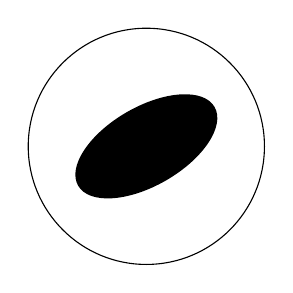
\begin{tikzpicture}
\draw (1,0) circle [radius=1.5];
\fill (1,0) circle [x radius=1cm, y radius=5mm, rotate=30];
\end{tikzpicture}

% 159
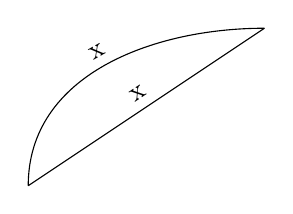
\begin{tikzpicture}
\draw (0,0) to [edge node={node [sloped,above] {x}}] (3,2);
\draw (0,0) to [out=90,in=180,
edge node={node [sloped,above] {x}}] (3,2);
\end{tikzpicture}

% 175
\tikz \shadedraw [shading=axis] (0,0) rectangle (1,1);
\tikz \shadedraw [shading=radial] (0,0) rectangle (1,1);
\tikz \shadedraw [shading=ball] (0,0) circle (.5cm);

% 234
\begin{tikzpicture}[level distance=8mm]
\node (root) {root}
child { node (a) {a} }
child { node (b) {b}
child { node (d) {d} }
child { node (e) {e} } }
child { node (c) {c} };
\begin{pgfonlayer}{background}
\node[fill=red!20,inner sep=0pt,ellipse,fit=(root) (b) (d) (e)] {};
\node[fill=blue!20,inner sep=0pt,ellipse,fit=(b) (c) (e)] {};
\end{pgfonlayer}
\end{tikzpicture}

% 238
\tikz [allow upside down]
\draw (0,0) .. controls +(up:2cm) and +(left:2cm) .. (1,3)
node foreach \p in {0,0.25,...,1} [sloped,above,pos=\p]{\p};

% 246
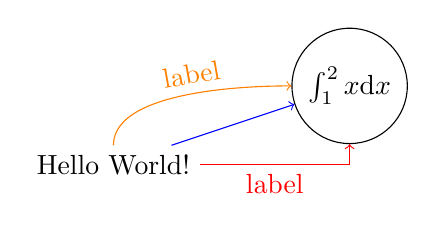
\begin{tikzpicture}
\path (0,0) node
 (x) {Hello World!}
(3,1) node[circle,draw](y) {$\int_1^2 x \mathrm d x$};
\draw[->,blue]
 (x) -- (y);
\draw[->,red]
 (x) -| node[near start,below] {label} (y);
\draw[->,orange] (x) .. controls +(up:1cm) and +(left:1cm) .. 
node[above,sloped] {label} (y);
\end{tikzpicture}

% % 249
% \begin{tikzpicture}[remember picture]
% \node (c) [circle,draw] {Big circle};
% \draw [overlay,->,very thick,red,opacity=.5]
% (c) to[bend left] (n1) (n1) -| (n2);
% \end{tikzpicture}

% % 346
% \tikzfading[name=fade inside,
% inner color=transparent!80,
% outer color=transparent!30]
% \begin{tikzpicture}
% % Checker board
% \fill [black!20] (0,0) rectangle (4,4);
% \path [pattern=checkerboard,pattern color=black!30] (0,0) rectangle (4,4);
% \shade [ball color=red] (3,3) circle (0.8);
% \shade [ball color=white,path fading=fade inside] (2,2) circle (1.8);
% \end{tikzpicture}

% 603
\begin{tikzpicture}
a big \draw [help lines] grid (3,2);
 \draw [red, dashed]
[postaction={decoration={text along path, text={a big juicy apple},
text align={align=right}}, decorate}]
 (0,0) .. controls (0,2) and (3,2) .. (3,0);
\end{tikzpicture}

% 754
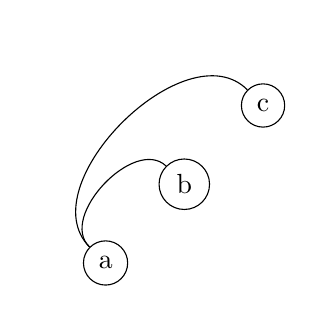
\begin{tikzpicture}[out=90,in=90,relative]
\node [circle,draw] (a) at (0,0) {a};
\node [circle,draw] (b) at (1,1) {b};
\node [circle,draw] (c) at (2,2) {c};
\path (a) edge (b)
edge (c);
\end{tikzpicture}

% % 841
% \tikz \datavisualization [
% school book axes,
% x axis={label=£x£},
% visualize as smooth line/.list={log, lin, squared, exp},
% every data set label/.append style={text colored},
% log= {pin in data={text’=£\log x£, when=y is -1}},
% lin= {pin in data={text=£x/2£, when=x is 2,
%       pin length=1ex}},
% squared={pin in data={text=£x^2£, when=x is 1.1,
%          pin angle=230}},
% exp= {label in data={text=£e^x£, when=x is -2}},
% style sheet=vary hue]
% data group {function classes};

\end{comment}
\begin{comment}

\chapter{Funzioni}

Riprendiamo ora il concetto di funzione, precedentemente studiato nel capitolo 
12 del secondo volume, approfondendone alcuni aspetti che ci saranno utili nel 
proseguo del nostro percorso.

\section{Definizione di funzione}
%label{}
\begin{definizione}
  Dati due insiemi $A$ e $B$ non vuoti definiti in $\mathbb{R}$ è detta 
$f$, \textsc{funzione reale di variabile reale}, una qualsiasi legge, 
applicazione o corrispondenza che associa a ogni elemento di $A$ uno e un 
solo elemento di $B$.
\end{definizione}

\begin{figure}[htpb!]
  \centering
  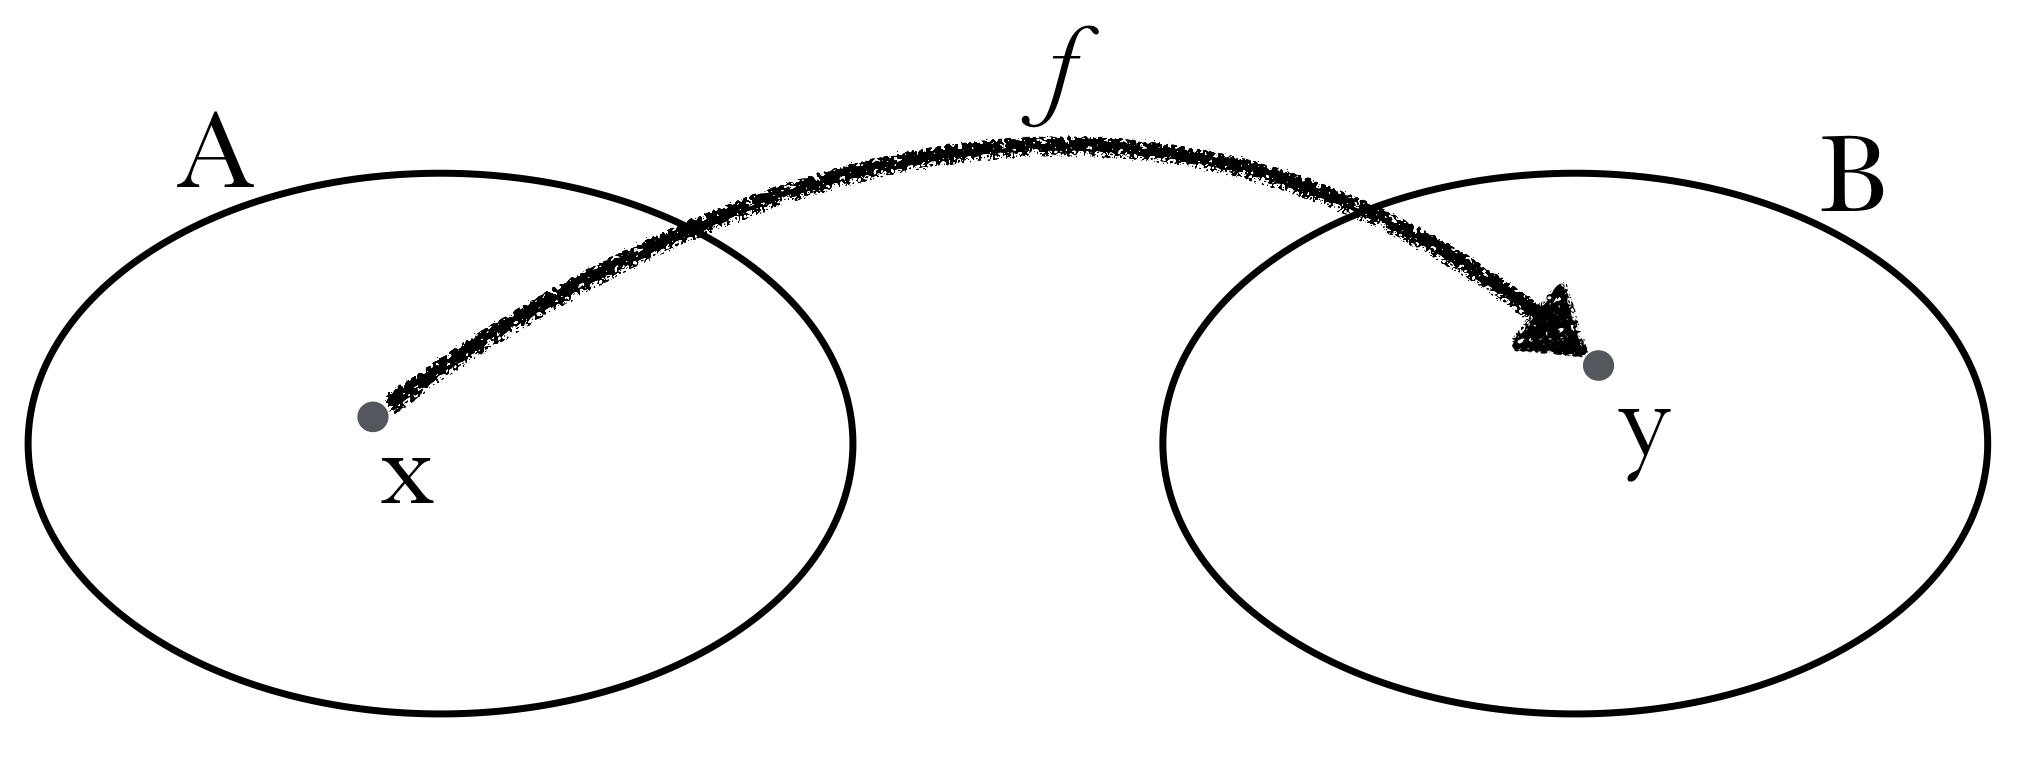
\includegraphics[width=0.55\textwidth]{img/1_funz.png}
  %%\caption{}
  %%\label{fig:1_1}
\end{figure}

Una funzione viene indicata:\\

$f: A\to B  $  tra insiemi   $f: x\mapsto y$   tra elementi  con $x\in A 
$  e $y\in B$\\

Dobbiamo pensare che $x$ mediante la corrispondenza $f$ diventa $y$, 
l'elemento $y$ è dunque l'\textsc{immagine} di $x$ mediante la trasformazione 
$f$; altrettanto e viceversa possiamo chiamare $x$ \textsc{controimmagine} di 
$y$.\\

L'elemento $x$ viene dunque proiettato mediante una sua trasformazione che 
chiamiamo $f$ nell'elemento $y$ di $B$, $y$ risulta così dipendente da $x$ 
perché determinata proprio in funzione di $x$, variabile indipendente.\\

L'immagine $y$ risulta propriamente in funzione di $x$ e possiamo scrivere 
$f(x)=y$ e la precedente espressione tra elementi diventa $f: x\mapsto 
f(x)=y$.\\

Definiamo $D$ \textsc{dominio} l'insieme $A$ delle $x$ e $C$ 
\textsc{codominio} il sottoinsieme di $B$ di tutte le immagini di $x$, cioè 
di tutte e sole le $y$ generate dalla trasformazione $f$.\\

\begin{figure}[htpb!]
  \centering
  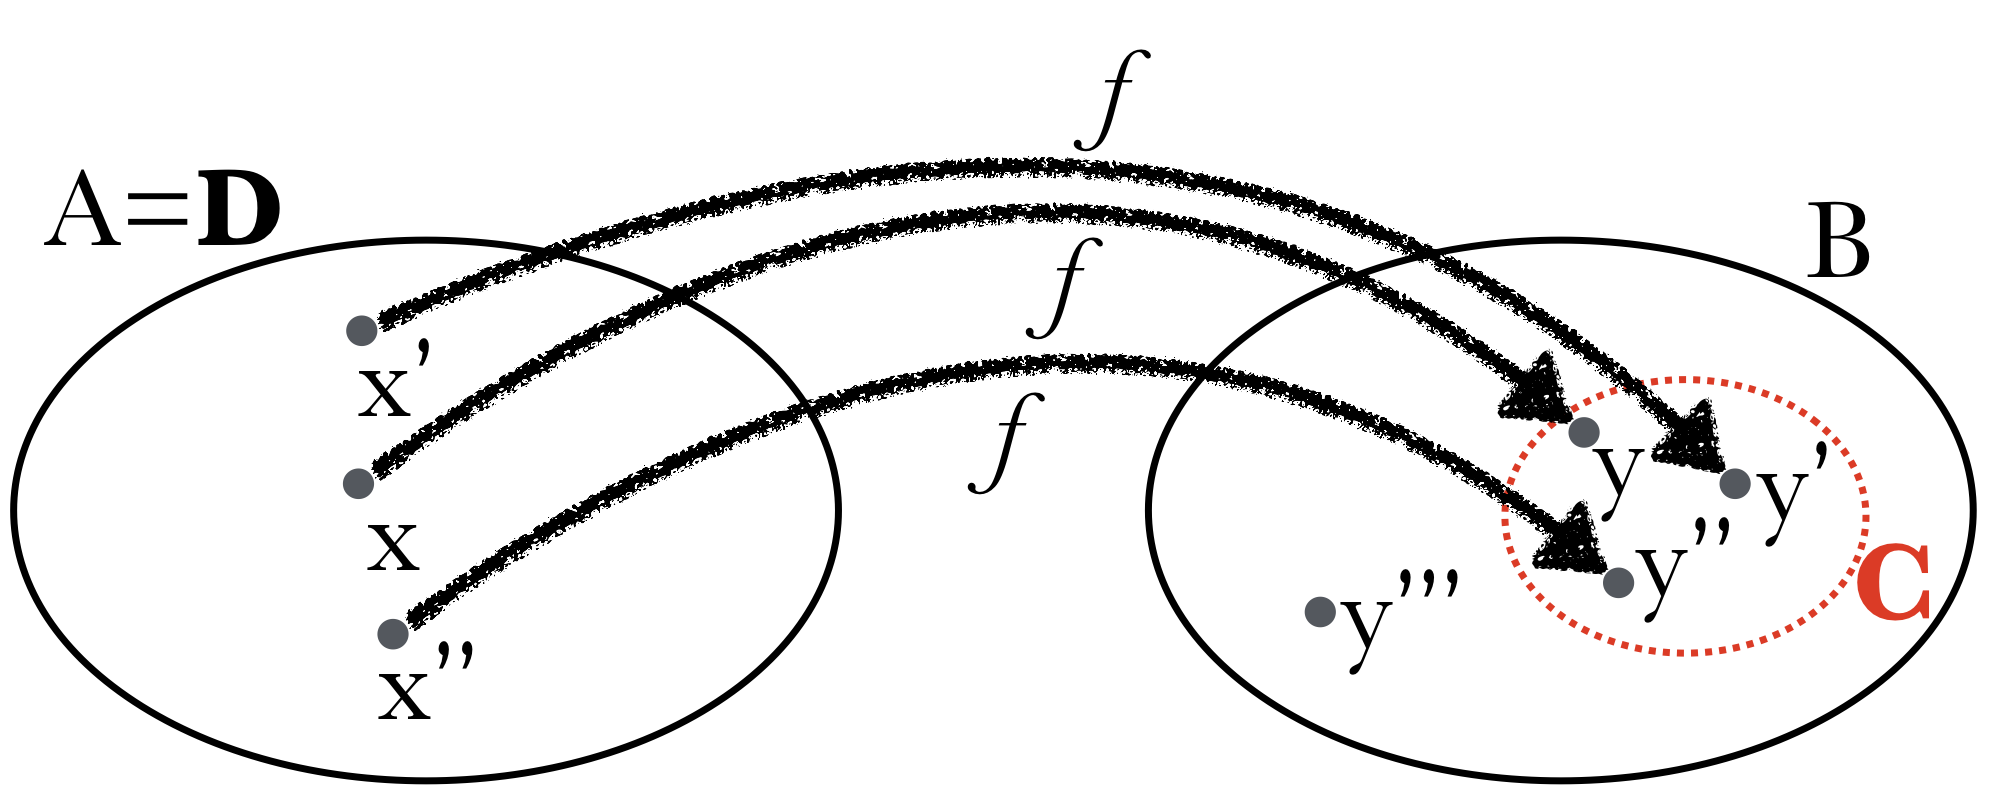
\includegraphics[width=0.55\textwidth]{img/2_funz.png}
  %\caption{}
  %\label{fig:1_2}
\end{figure}
%
Notiamo, nella figura precedente che mentre il dominio coincide con l'insieme 
di partenza il codominio è un sottoinsieme dell'insieme di arrivo.\\

%
%
%
\begin{esempio}
  Visualizziamo dominio e codominio della funzione $f(x)=x^2$
  \begin{figure}[htpb!]
  \centering
  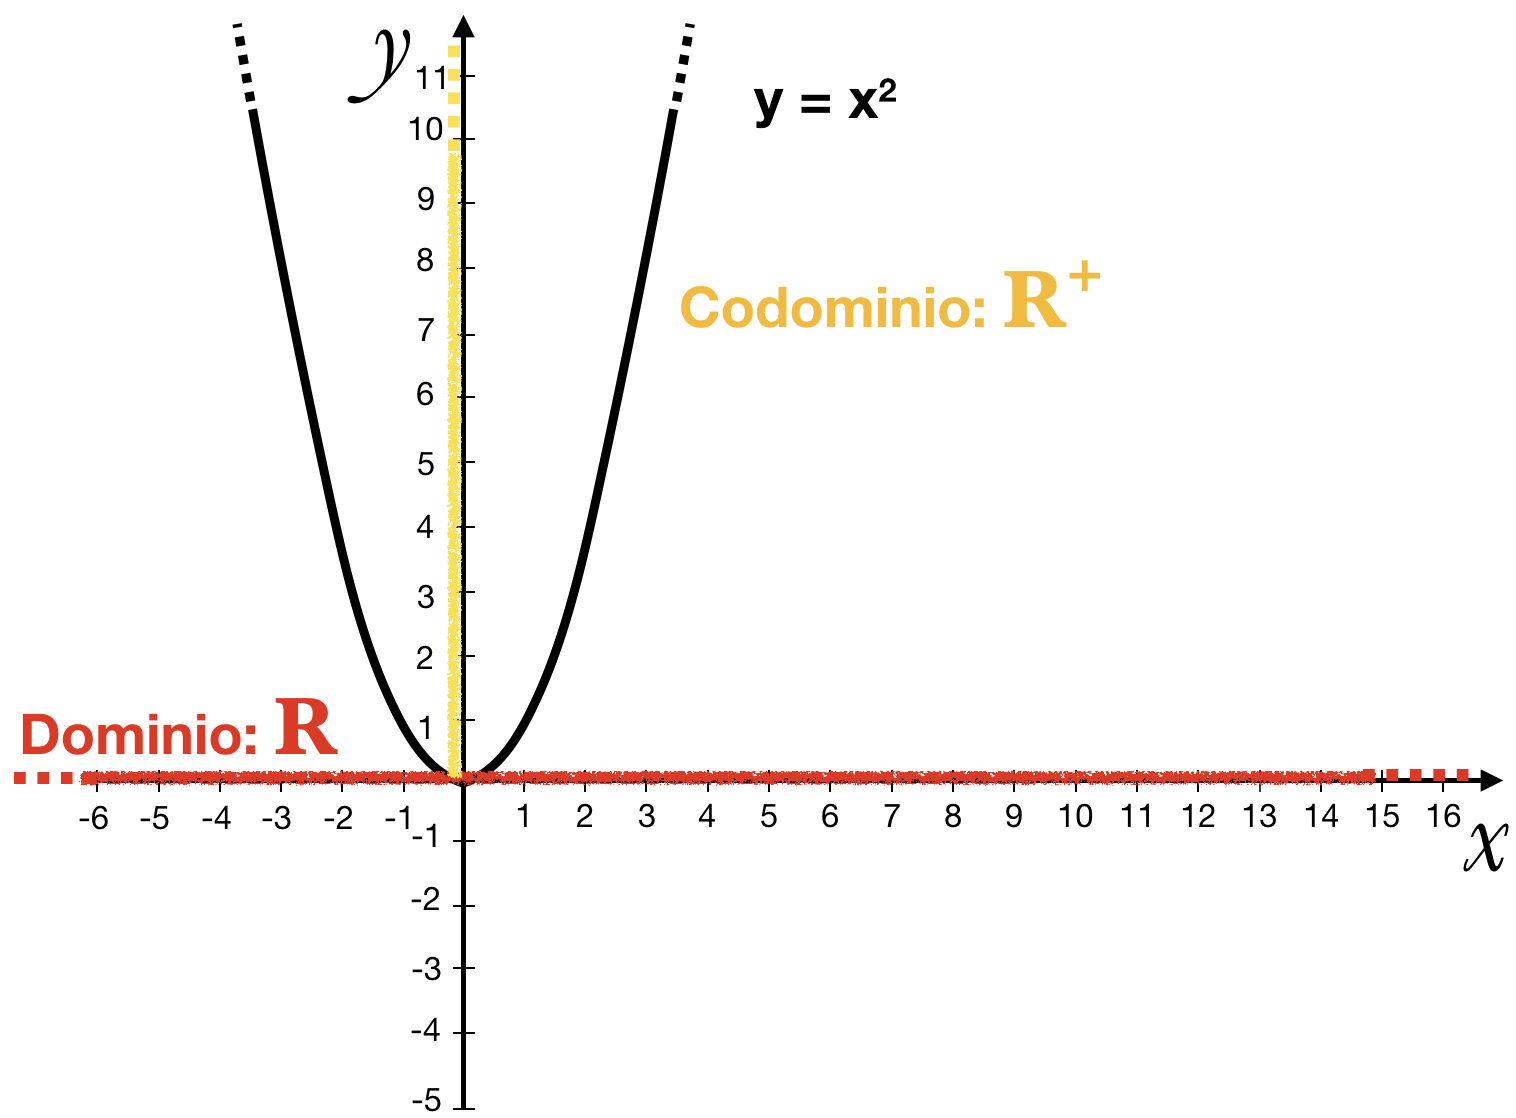
\includegraphics[width=0.4\textwidth]{img/2a_funz.png}
  %\caption{}
  %\label{fig:1_2}
  \end{figure}
\end{esempio}

\begin{esempio}
  Visualizziamo dominio e codominio della funzione $f(x)=\log{x}$
  \begin{figure}[htpb!]
  \centering
  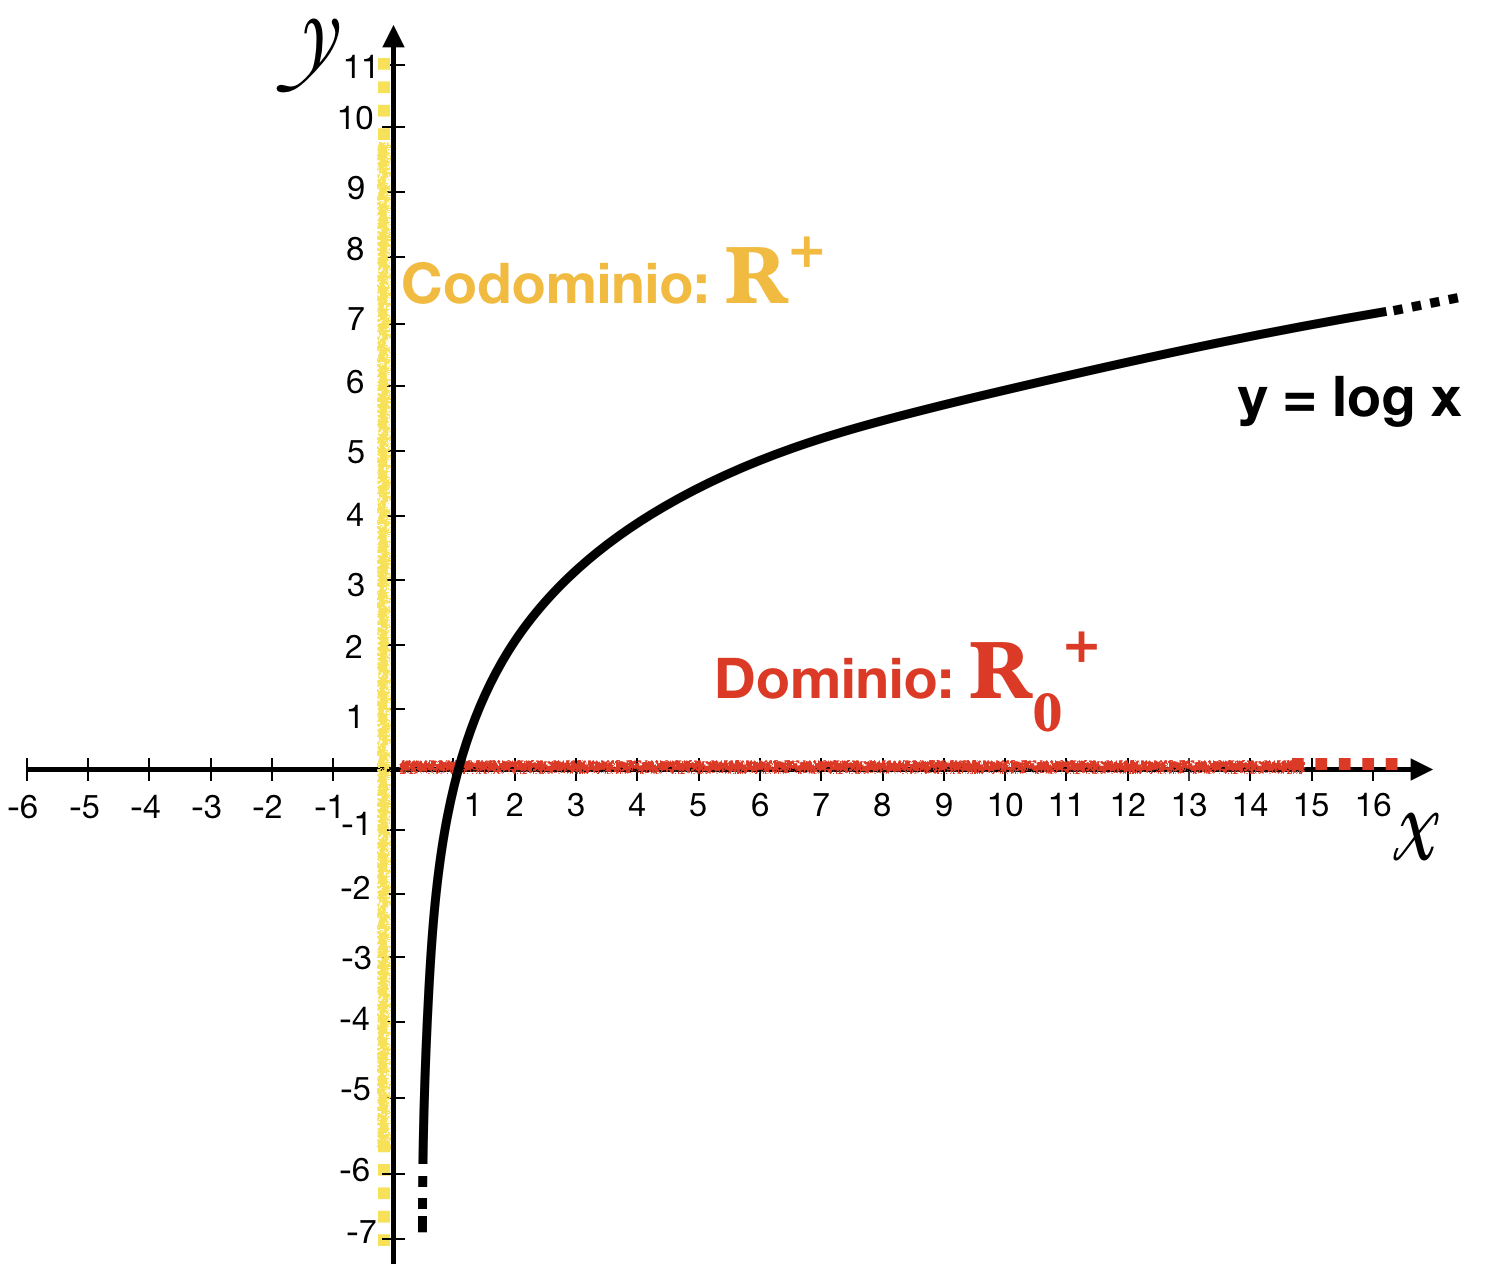
\includegraphics[width=0.4\textwidth]{img/2b_funz.png}
  %\caption{}
  %\label{fig:1_2}
  \end{figure}
\end{esempio}

\begin{esempio}
  Visualizziamo dominio e codominio della funzione $f(x)=\frac{9}{x}$
  \begin{figure}[htpb!]
  \centering
  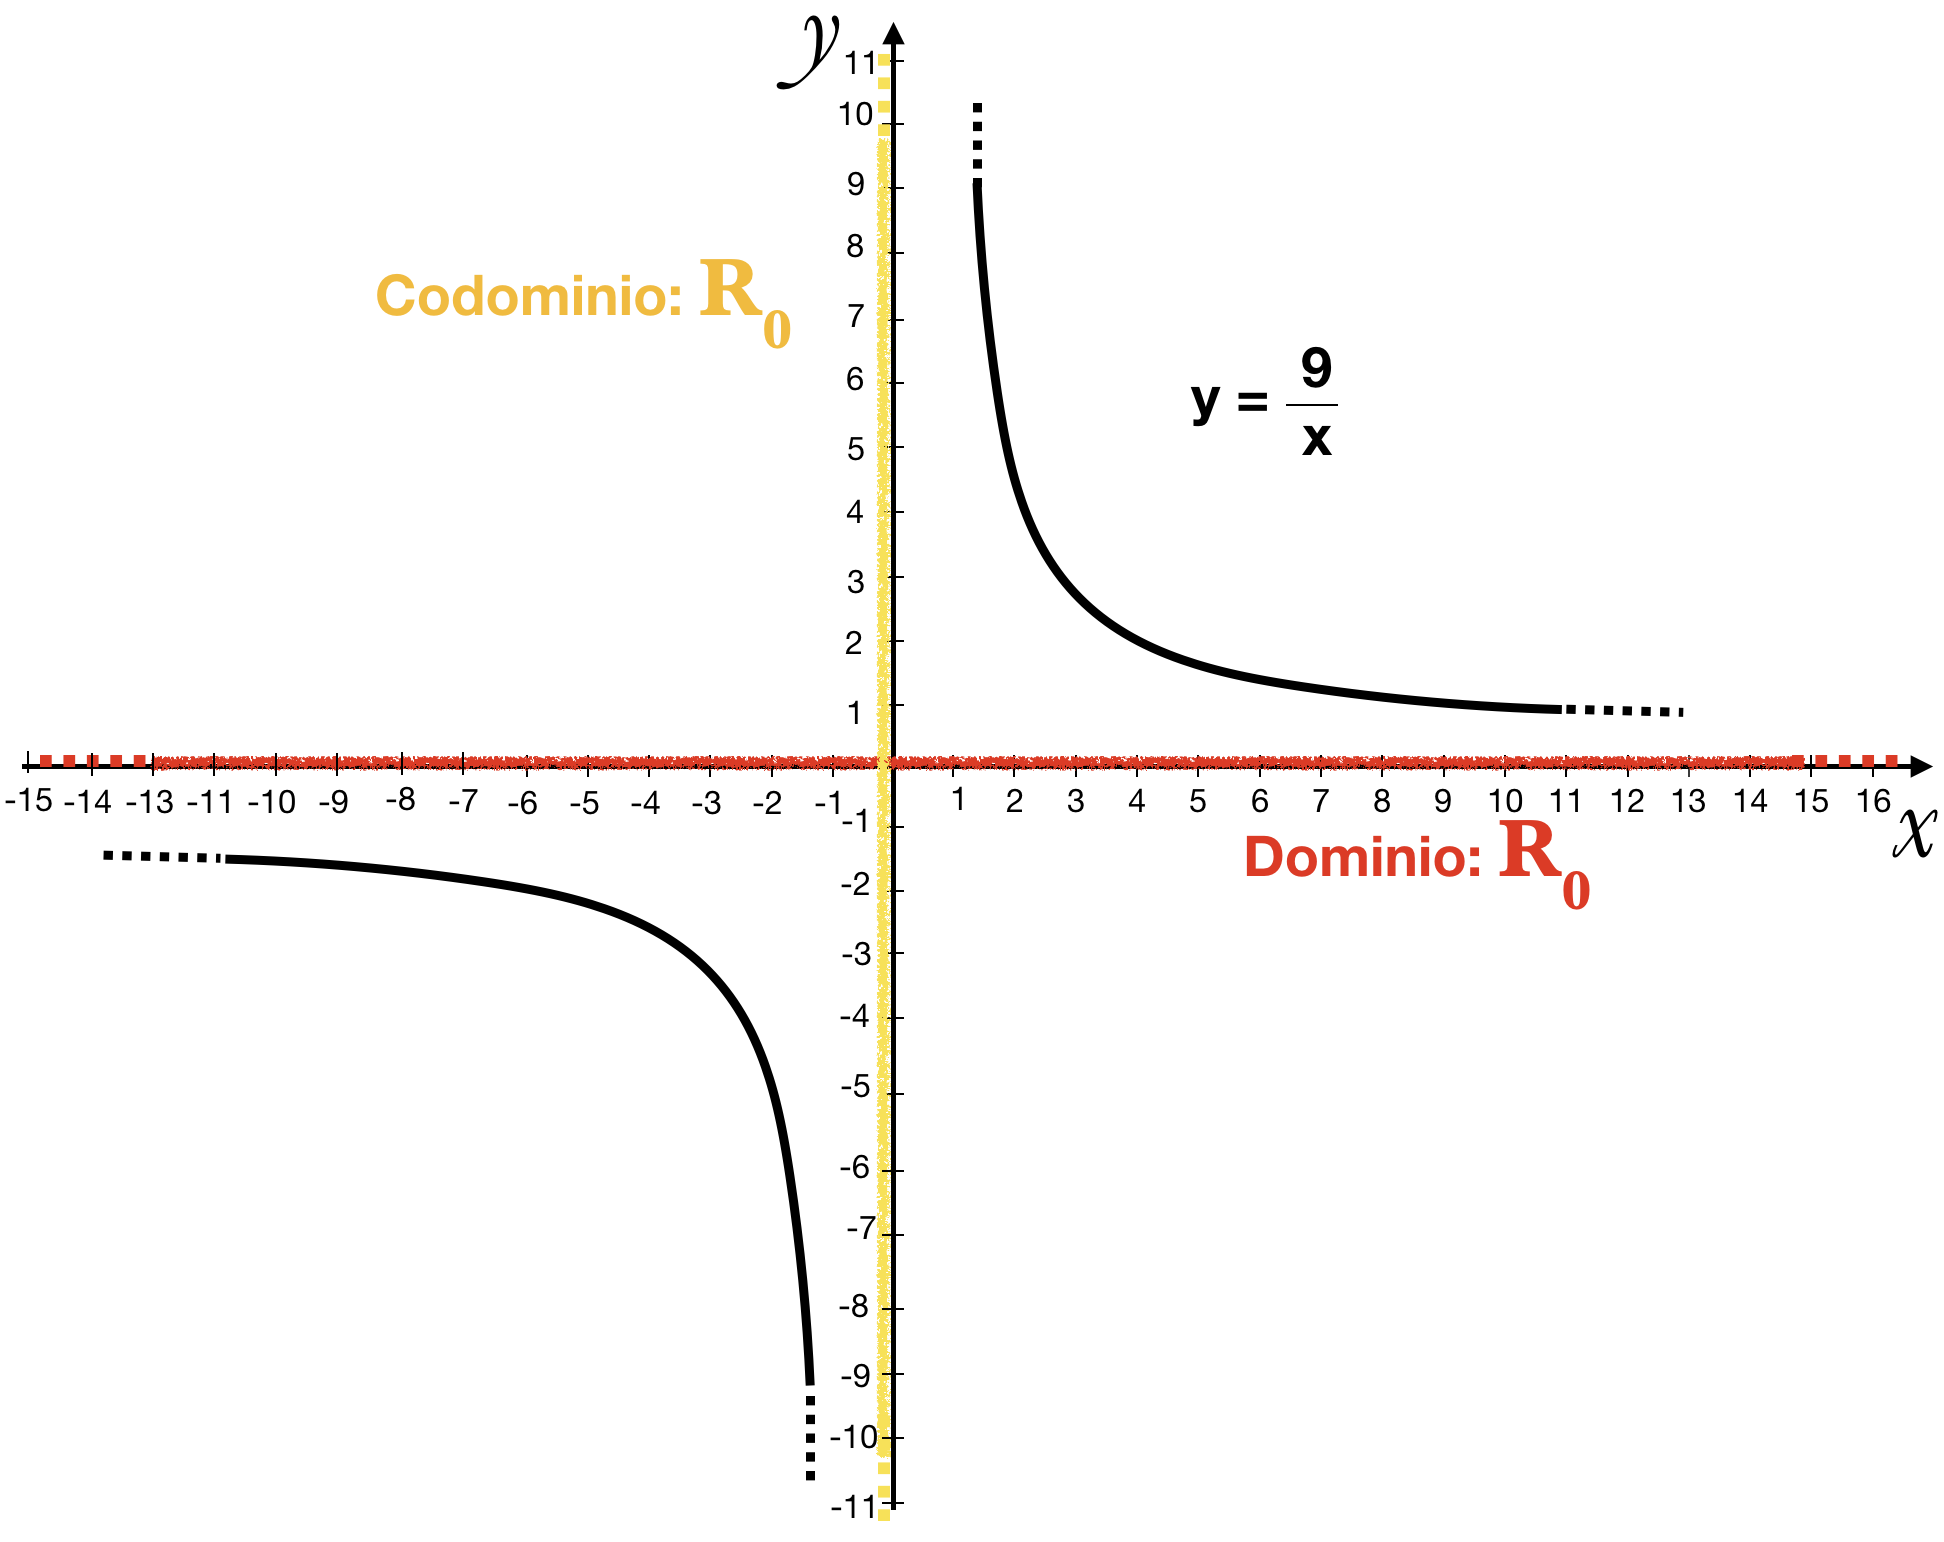
\includegraphics[width=0.55\textwidth]{img/2c_funz.png}
  %\caption{}
  %\label{fig:1_2}
  \end{figure}
\end{esempio}

\newpage 
Per calcolare il dominio delle funzioni, vediamo una tabella riassuntiva dei 
possibili casi.\\

%%%%%%%%%%%%%%TABELLA DOMINIO FUNZIONI%%%%%%%%%%%%
\begin{table}

\raggedleft
%   \begin{tabularx}{1,2\textwidth}{XXX}
  \begin{tabularx}{\textwidth}{XXX}
  \toprule
  Funzione & Dominio  & Esempio \\
  \midrule
  
  \textbf{Funzioni razionali intere} 
\newline$y=a_0x^n+a_1x^{n-1}+\dots+a_n$ 
  & $\,$ \newline $D=\mathbb{R}$ 
  & $\,$ \newline $y=x^3-x^2+2x+1$ \newline $D=\mathbb{R}$ \\
  \midrule

  \textbf{Funzioni razionali fratte} \newline 
$y=\frac{A(x)}{B(x)}$ \newline con $A(x)$ e $B(x)$ polinomi 
  & $\mathbb{R}$ esclusi i valori che annullano $B(x)$, cioè 
\newline $B(x)\neq 0$
  & $\,$ \newline$y=\frac{3+x^2}{x-5}$\newline $D= 
\mathbb{R}-\{5\}$ \\
  \midrule

  \textbf{Funzioni irrazionali} \newline $y=\sqrt[n]{f(x)}$ 
\newline con $n\in\mathbb{N},\,n>1$ 
  & $\,$ \newline Se $n$ è dispari il $D$ è il $D$ di $f(x)$ 
\newline \newline Se $n$ è pari, \newline$D=\{x\in\mathbb{R}\vert f(x)\geq0\}$
  & $\,$ \newline $y=\sqrt[3]{x^2-9}$\newline $D=\mathbb{R}$ 
\newline \newline $y=\sqrt{x^2-1}$\newline $D=x^2\geq1=$\newline 
$=x\leq-1\lor x\geq1$ \\
  \midrule
  
  \textbf{Funzioni logaritmiche} \newline $y=\log_af(x)$ 
\newline con $a>0,\,a\neq1$ \newline \newline $y=\log_{g(x)}(f(x))$ 
  & $\,$ \newline $D=\{x\in\mathbb{R}\vert f(x)>0\}$\newline 
\newline \newline$D=\{x\in\mathbb{R}\vert f(x)>0\land$\newline$\land 
g(x)>0\land g(x)\neq1\}$
  & $\,$ \newline $y=\log(x+1)$\newline $D=x>-1$\\
  \midrule
  
   \textbf{Funzioni esponenziali} \newline $y=a^{f(x)}$ 
\newline con $a>0,\,a\neq1$ \newline\newline  $y={f(x)}^{g(x)}$ 
  & $\,$ \newline $D$ di $f(x)$ \newline \newline \newline 
$D=\{x\in\mathbb{R}\vert f(x)>0\}\land$ $D$ di $g(x)$
  &  $\,$ \newline$y=3^{2x}$\newline $D= \mathbb{R}$ \newline  
\newline$y=e^{\frac{1}{x+1}}$ \newline $D=\mathbb{R}-\{-1\}$ \\
  \midrule
  
  \textbf{Funzioni potenza} \newline $y=f(x)^a$ \newline con 
$a\in\mathbb{R},\,a\neq0$ \newline \newline$a$ intero positivo \newline 
\newline $a$ intero negativo \newline  \newline $a$ razionale \newline  
\newline$a$ irrazionale positivo \newline \newline $a$ irrazionale negativo 
  & $\,$  \newline  \newline  \newline  \newline  $D$ di $f(x)$ 
\newline  \newline $D$ di $f(x)$ con $f(x)\neq0$\newline \newline $D$ di 
$f(x)$ razionale \newline \newline $D=\{x\in\mathbb{R}\vert 
f(x)\geq0\}$\newline \newline $D=\{x\in\mathbb{R}\vert f(x)>0\}$
  & $\,$  \newline  \newline  \newline  \newline $y=(x-1)^2$ 
$D=\mathbb{R}$ \newline \newline $y=(x-1)^{-2}$ $D=x\neq1$ \newline \newline 
$y=(x-1)^{1/2}=\sqrt{x-1}$ $D=x\geq1$ \newline $y=(x-1)^{\pi}$ $D=x\geq1$ 
\newline \newline $y=(x-1)^{-\pi}$ $D=x>1$\\
  \midrule

  \textbf{Funzioni goniometriche} \newline $y=\sin{x}$, 
$y=\cos{x}$ \newline \newline $y=\tan x$, $y=\sec x$ \newline  \newline 
$y=\cot x$, $y=\csc x$ 
  & $\,$ \newline $D=\mathbb{R}$ \newline  \newline 
$D=\mathbb{R} -\bigl\{\frac{\pi}{2}+k\pi \bigr\}$\newline \newline 
$D=\mathbb{R} -\{k\pi\}$
  &  \\
  \midrule
  
\end{tabularx}
\end{table}

\begin{table}   

\raggedleft   
\begin{tabularx}{\textwidth}{XXX}
  \midrule

  \textbf{Funzioni goniometriche inverse} \newline 
$y=\arcsin{x}$, $y=\arccos{x}$ \newline \newline $y=\arctan x$, 
$y=\text{arccot}\,x$
  & $\,$ \newline \newline $D=[-1,1]$ \newline  \newline 
$D=\mathbb{R}$
  &  \\
  \midrule

  \textbf{Funzioni goniometriche composte} \newline 
$y=\sin[f(x)]$, $y=\cos [f(x)]$ \newline \newline $y=\tan [f(x)]$ \newline 
\newline \newline $y=\cot [f(x)]$ \newline  \newline $y=\arcsin[f(x)]$, 
\newline $y=\arccos [f(x)]$ \newline \newline $y=\arctan [f(x)]$
  & $\,$ \newline \newline $D$ di $f(x)$ \newline  \newline 
$D=\bigl\{x\in\mathbb{R}\vert f(x)\neq\frac{\pi}{2}+\newline+k\pi 
\bigr\}$\newline \newline $D=\{x\in\mathbb{R}\vert f(x)\neq k\pi\}$ \newline 
\newline $D=\{x\in\mathbb{R}\vert -1\leq f(x)\leq\newline\leq1\}$ \newline 
\newline $D$ di $f(x)$
  & $\,$ \newline \newline \newline $y=\tan[2x-1]$ \newline 
$2x-1\neq \frac{\pi}{2}+k\pi$ \newline$D=x\neq\frac{\pi+1+k\pi}{2}$  \newline 
\newline \newline  $y=\arcsin[x-1]$ \newline $-1\leq x-1\leq1$\newline $0\leq 
x\leq2$\newline \newline$y=\arctan [\frac{x+2}{x+3}]$ \newline 
$D=\mathbb{R}-\{-3\}$
 \\

  \bottomrule
\end{tabularx}
\end{table}
\newpage

\section{La rappresentazione di una funzione}
%label{}
Una funzione può essere rappresentata in diversi modi, i principali sono:
\begin{itemize}
  \item \textsc{Rappresentazione tabulare}\\
Le funzioni empiriche vengono ricostruite con una tabella in cui ad ogni $y$ 
corrisponde un certo $x$. Ad esempio pensiamo ad una tabella che dà la 
temperatura ora per ora in un certo luogo.
%
  \item \textsc{Rappresentazione analitica}\\
La funzione è espressa mediante un insieme di operazioni matematiche che 
applicate in un certo ordine ad $x$ restituiscono un corrispondente valore di 
$y$. Esempi ne sono $y=\log{(x+2)}$, $y=2x^3+3$ o $y=\sin{x}+2^x$, cioè le 
espressioni, scritte in linguaggio matematico, che siamo abituati a trattare.
%
  \item \textsc{Rappresentazione grafica}\\
La funzione è rappresentata come una corrispondenza $x-$y su un grafico 
cartesiano; in particolare, ricordiamo che: il grafico di una funzione $f 
:A\to B$ è l'insieme di tutte le coppie ordinate $(x;y)$ che si ottengono 
prendendo un valore $x$ in $A$ e trovando il corrispondente valore $y=f(x)$ 
in $B$. Ogni coppia ordinata rappresenta un punto nel piano cartesiano 
$\mathbb{R}^2$.
\end{itemize}

\section{Le proprietà di una funzione}
%label{}
Una funzione, a seconda, del modo in cui gli elementi del dominio 
corrispondono agli elementi del codominio si può definire \textsc{iniettiva}, 
\textsc{suriettiva} e \textsc{biiettiva} (o \textsc{biunivoca}).\\

\begin{definizione}
Una funzione da $A$ a $B$ si dice \textsc{iniettiva} se ogni elemento di $B$ 
è immagine di \underline{al più} un elemento di $A$;\\


$f : A\to B$ è iniettiva se  $\forall x_1,\,x_2\in A ,\,x_1\neq 
x_2\Rightarrow f(x_1 )\neq f(x_2)$
\end{definizione}

\begin{figure}[htpb!]
  \centering
  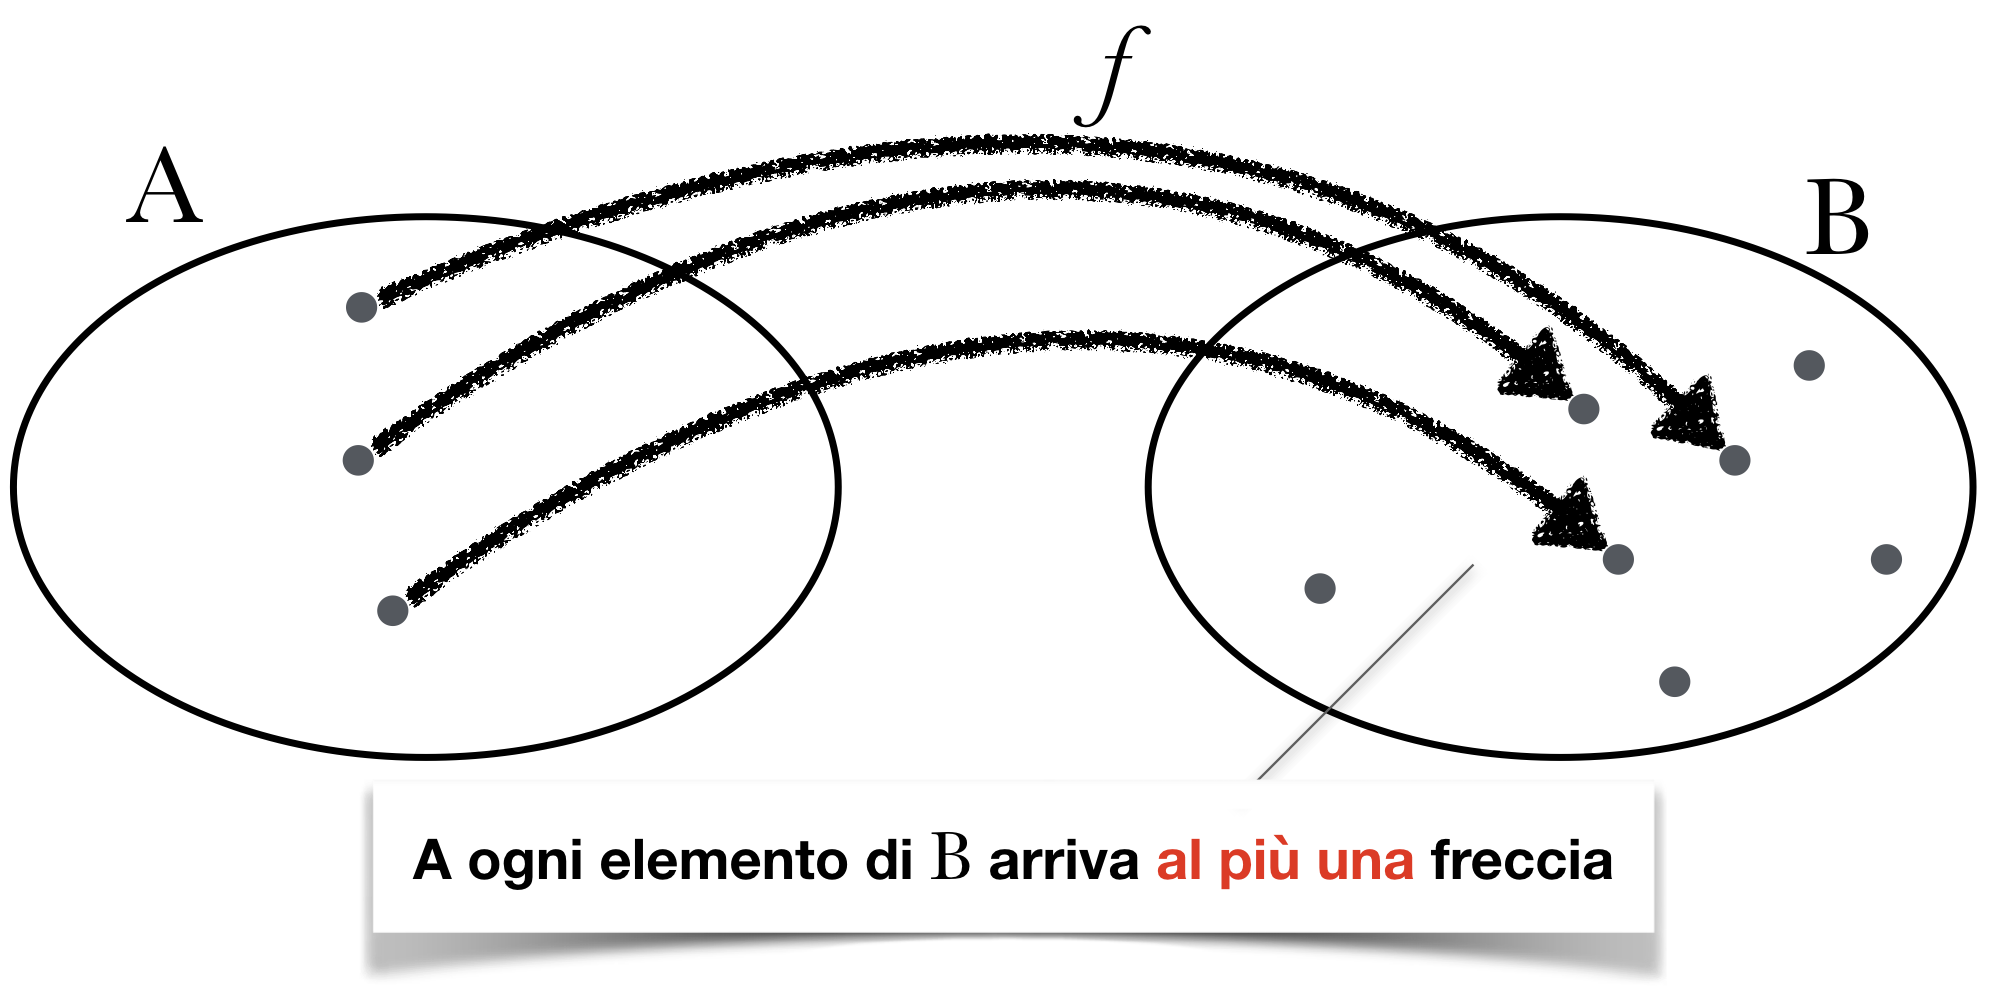
\includegraphics[width=0.55\textwidth]{img/3_funz.png}
  %\caption{}
  %\label{fig:1_2}
\end{figure}

\begin{definizione}
Una funzione da $A$ a $B$ si dice \textsc{suriettiva} quando ogni elemento di 
$B$ è immagine di \underline{almeno un} elemento di $A$;\\

$f: A\to B$ è suriettiva se $\forall y\in B, \exists x\in A \mid f(x)=y$
\end{definizione}

\begin{figure}[htpb!]
  \centering
  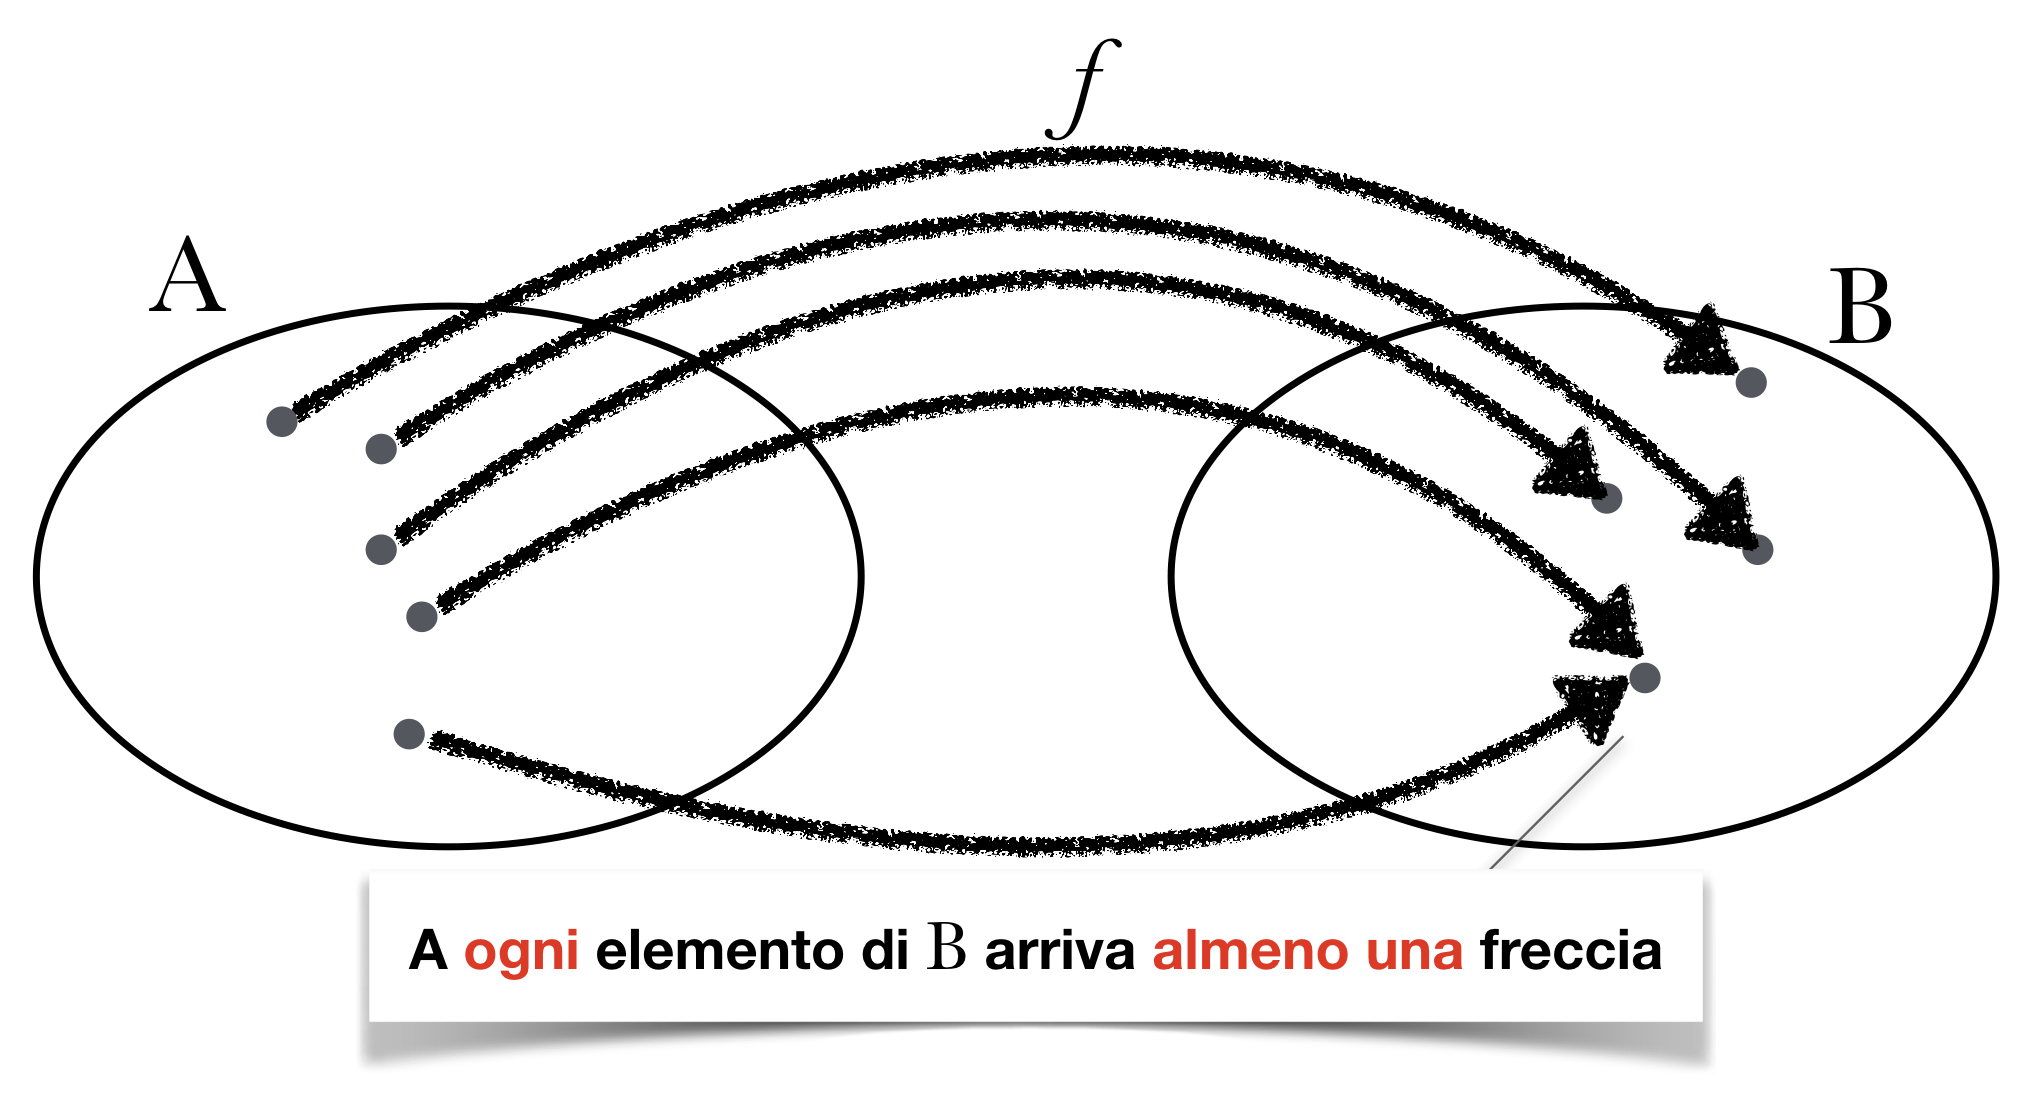
\includegraphics[width=0.55\textwidth]{img/4_funz.png}
  %\caption{}
  %\label{fig:1_2}
\end{figure}

Il fatto che una funzione sia o non sia suriettiva dipende da come si sceglie 
l'insieme di arrivo. Se lo si sceglie coincidente con il codominio la 
funzione è suriettiva.\\
%
\begin{definizione}
Una funzione da $A$ a $B$ è \textsc{biiettiva} (o \textsc{biunivoca}) quando 
è sia iniettiva sia suriettiva.\\
\end{definizione}

\begin{figure}[htpb!]
  \centering
  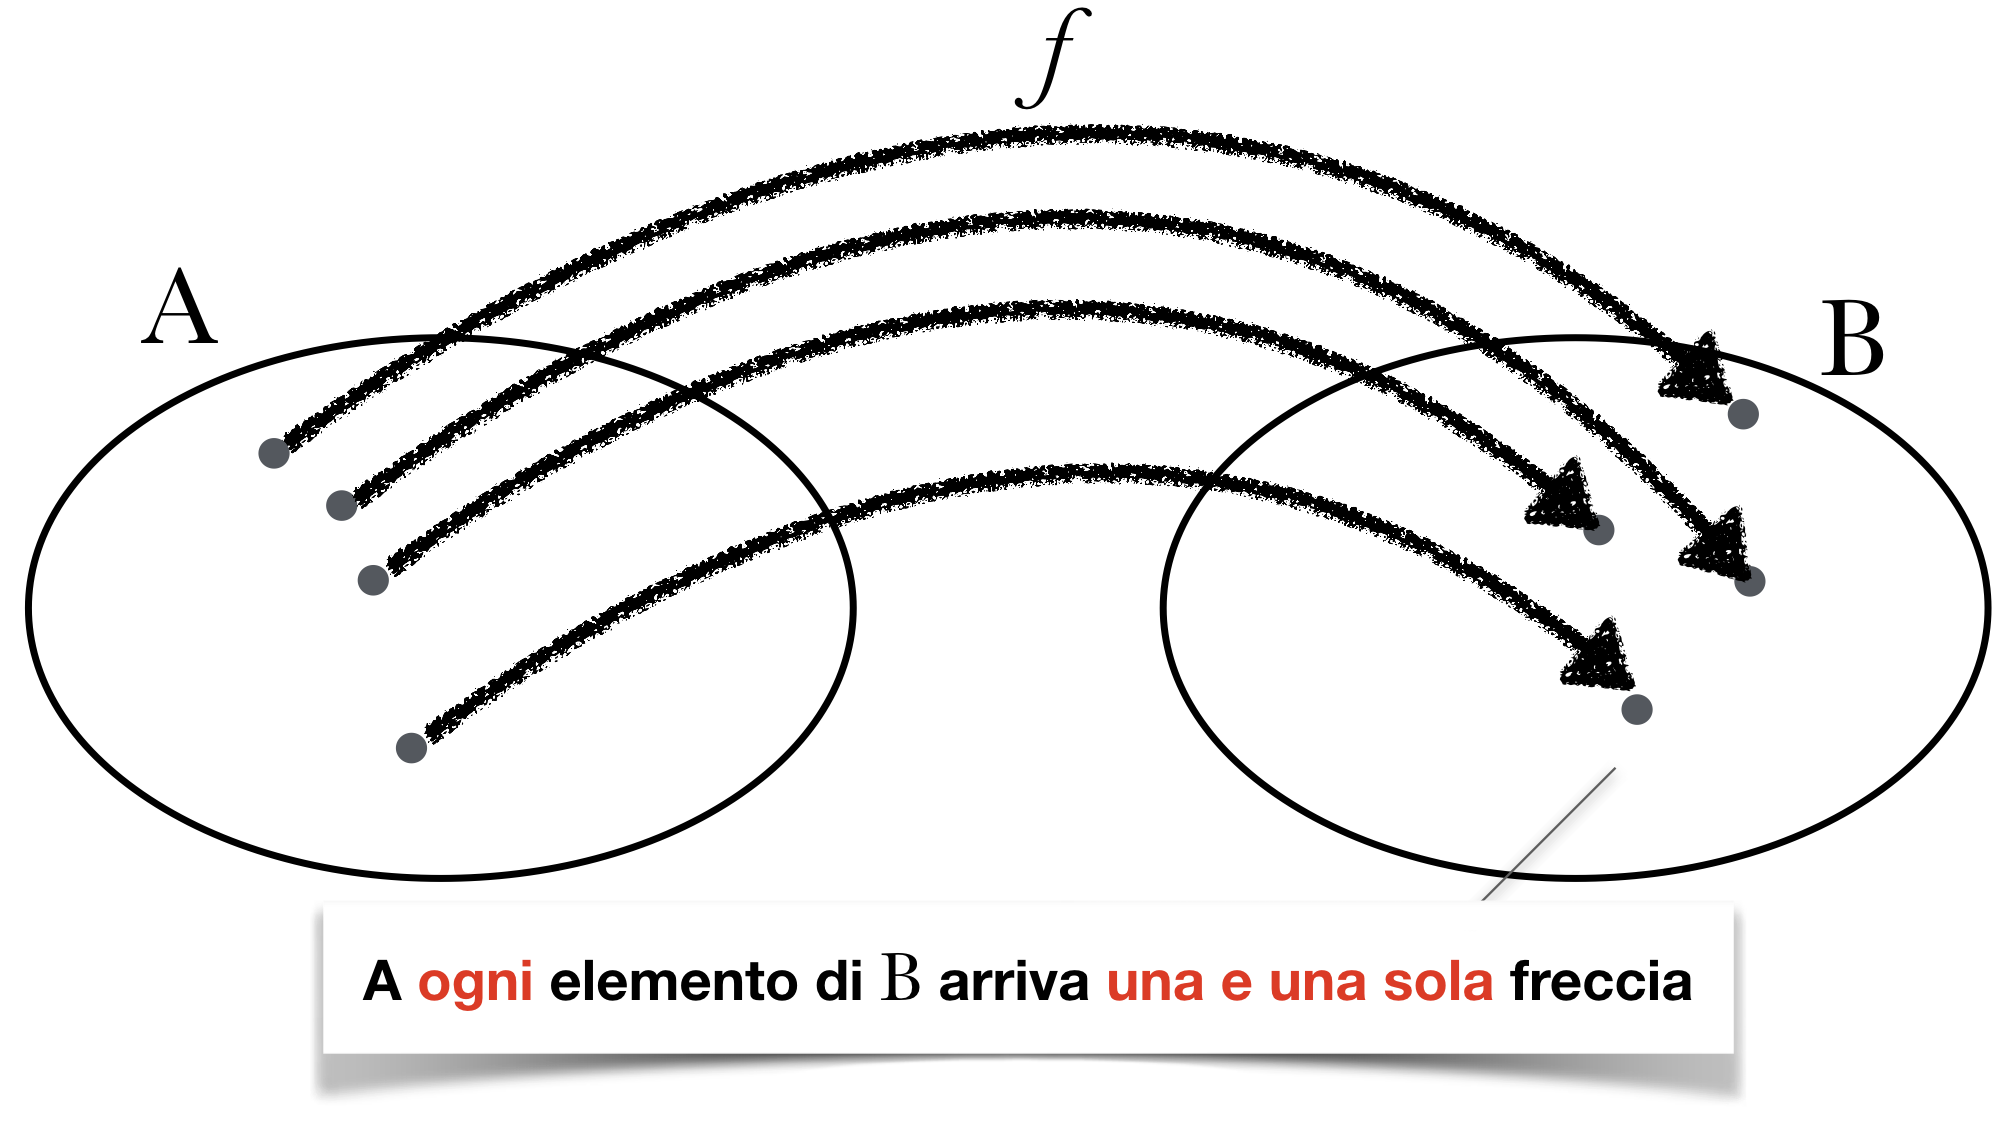
\includegraphics[width=0.55\textwidth]{img/5_funz.png}
  %\caption{}
  %\label{fig:1_2}
\end{figure}

\begin{esempio} Quando una funzione è biettiva?\\
Una funzione biiettiva è ad esempio una qualsiasi retta. Una retta è infatti 
sia iniettiva, che biettiva di dominio $\mathbb{R}$ e codominio 
$\mathbb{R}$.\\
\end{esempio}

Una funzione biiettiva viene anche detta biiezione o corrispondenza biunivoca 
fra gli insieme $A$ e $B$. Tale relazione tra insiemi è molto forte e 
specifica in quanto ad ogni elemento di $A$ viene associato un solo elemento 
di $B$ e, reciprocamente, ad ogni elemento di $B$ è associato un solo 
elemento di $A$, in una relazione uno a uno. Per tale ragione, la relazione 
tra i due insiemi viene indicata con una doppia freccia $A\leftrightarrow B$.
%
\section{Le caratteristiche di una funzione}
%label{}
Analizziamo ora le caratteristiche che può manifestare una funzione, qualità 
che può presentare il suo andamento e che possono contraddistinguerne la 
forma del grafico.

\subsection{Monotonia}
%label{}
La caratteristica della monotonia vuole evidenziare l'andamento 
\textsc{crescente} o \textsc{decrescente} di una funzione; la monotonia 
studia il comportamento della variabile dipendente $y$ all'aumentare della 
variabile indipendente $x$. All'aumentare dell'ascissa se aumenta anche 
l'ordinata diremo che la funzione cresce, se l'ordinata diminuisce diremo che 
la funzione decresce. Vediamo e puntualizziamo meglio.\\

\begin{definizione}
Una funzione $y=f(x)$ di dominio $D$, si dice \textsc{crescente in senso 
stretto} in un intervallo $I$, sottoinsieme di $D$, se\\

$\forall x_1,x_2\in I$  con $x_1<x_2 $ si ha $f(x_1)<f(x_2)$\\
\end{definizione}

\begin{figure}[htpb!]
  \centering
  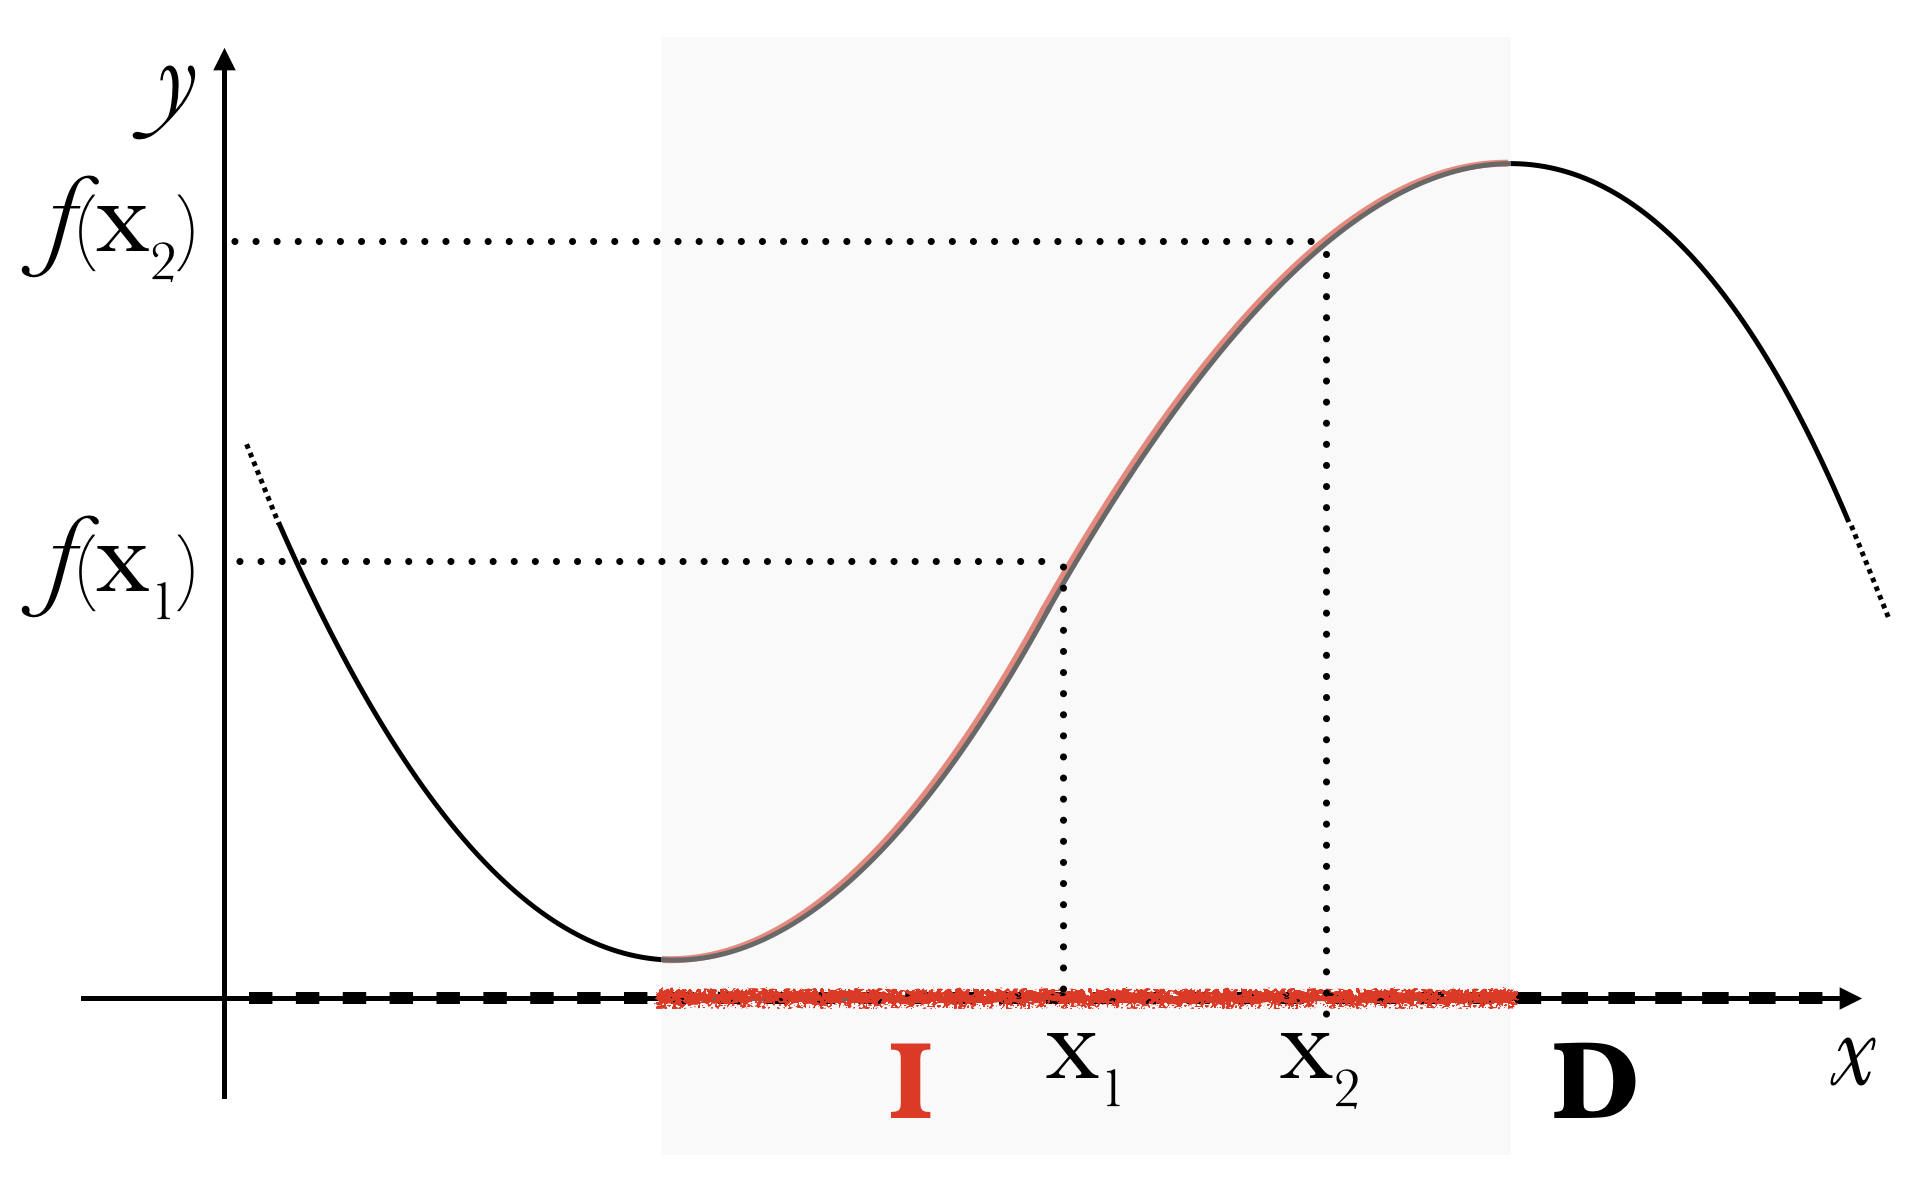
\includegraphics[width=0.55\textwidth]{img/funz_6.png}
  %\caption{}
  %\label{fig:1_2}
\end{figure}
%
\begin{definizione}
Una funzione è non decrescente o \textsc{crescente} in senso lato in un 
intervallo $I$, sottoinsieme di $D$, se\\

$\forall x_1,x_2\in I$  con $x_1<x_2 $ si ha $f(x_1)\leq f(x_2)$\\
%
\end{definizione}
%
%
%

\begin{definizione}
Una funzione $y=f(x)$ di dominio $D$, si dice \textsc{decrescente in senso 
stretto}, in un intervallo $I$, sottoinsieme di $D$, se\\

$\forall x_1,x_2\in I$  con $x_1<x_2 $ si ha $f(x_1)> f(x_2)$\\

\end{definizione}

\begin{figure}[htpb!]
  \centering
  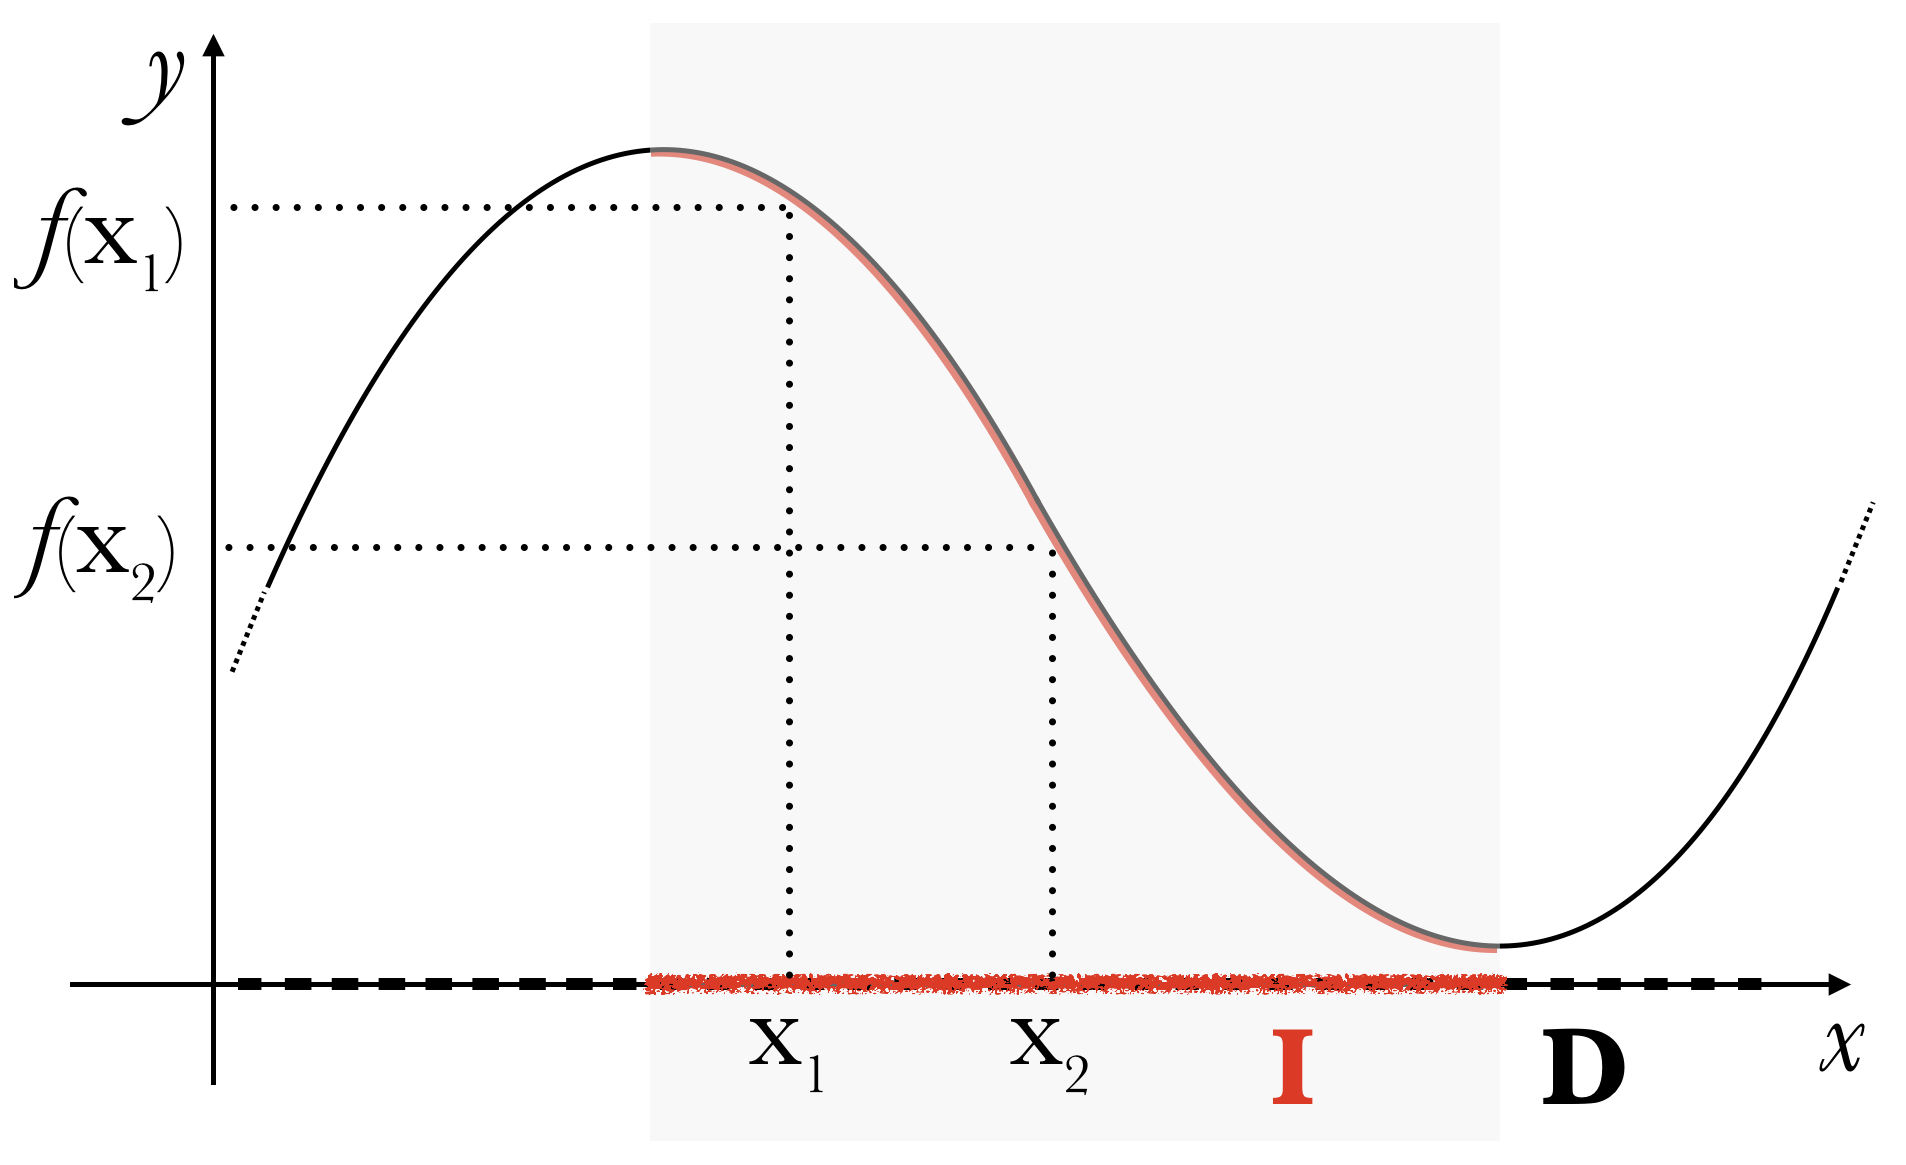
\includegraphics[width=0.55\textwidth]{img/funz_7.png}
  %\caption{}
  %\label{fig:1_2}
\end{figure}
%

\begin{definizione}
Una funzione è non crescente o \textsc{decrescente} in senso lato in un 
intervallo $I$, sottoinsieme di $D$, se\\

$\forall x_1,x_2\in I$  con $x_1<x_2 $ si ha $f(x_1)\geq f(x_2)$\\
\end{definizione}

Una funzione, quindi, si dice monotòna in un intervallo $I$ del suo dominio 
se in $I$ è sempre crescente o decrescente.\\

\begin{esempio}
Individuiamo gli intervalli in cui la funzione rappresentata risulta 
crescente o decrescente.\\
Negli intervalli finiti $x_1<x<x_2$, $x_3<x<x_4$ la funzione risulta essere 
crescente; negli intervalli finiti $x_2<x<x_3$, $x_4<x<x_5$.
% 
\begin{figure}[htpb!]
  \centering
  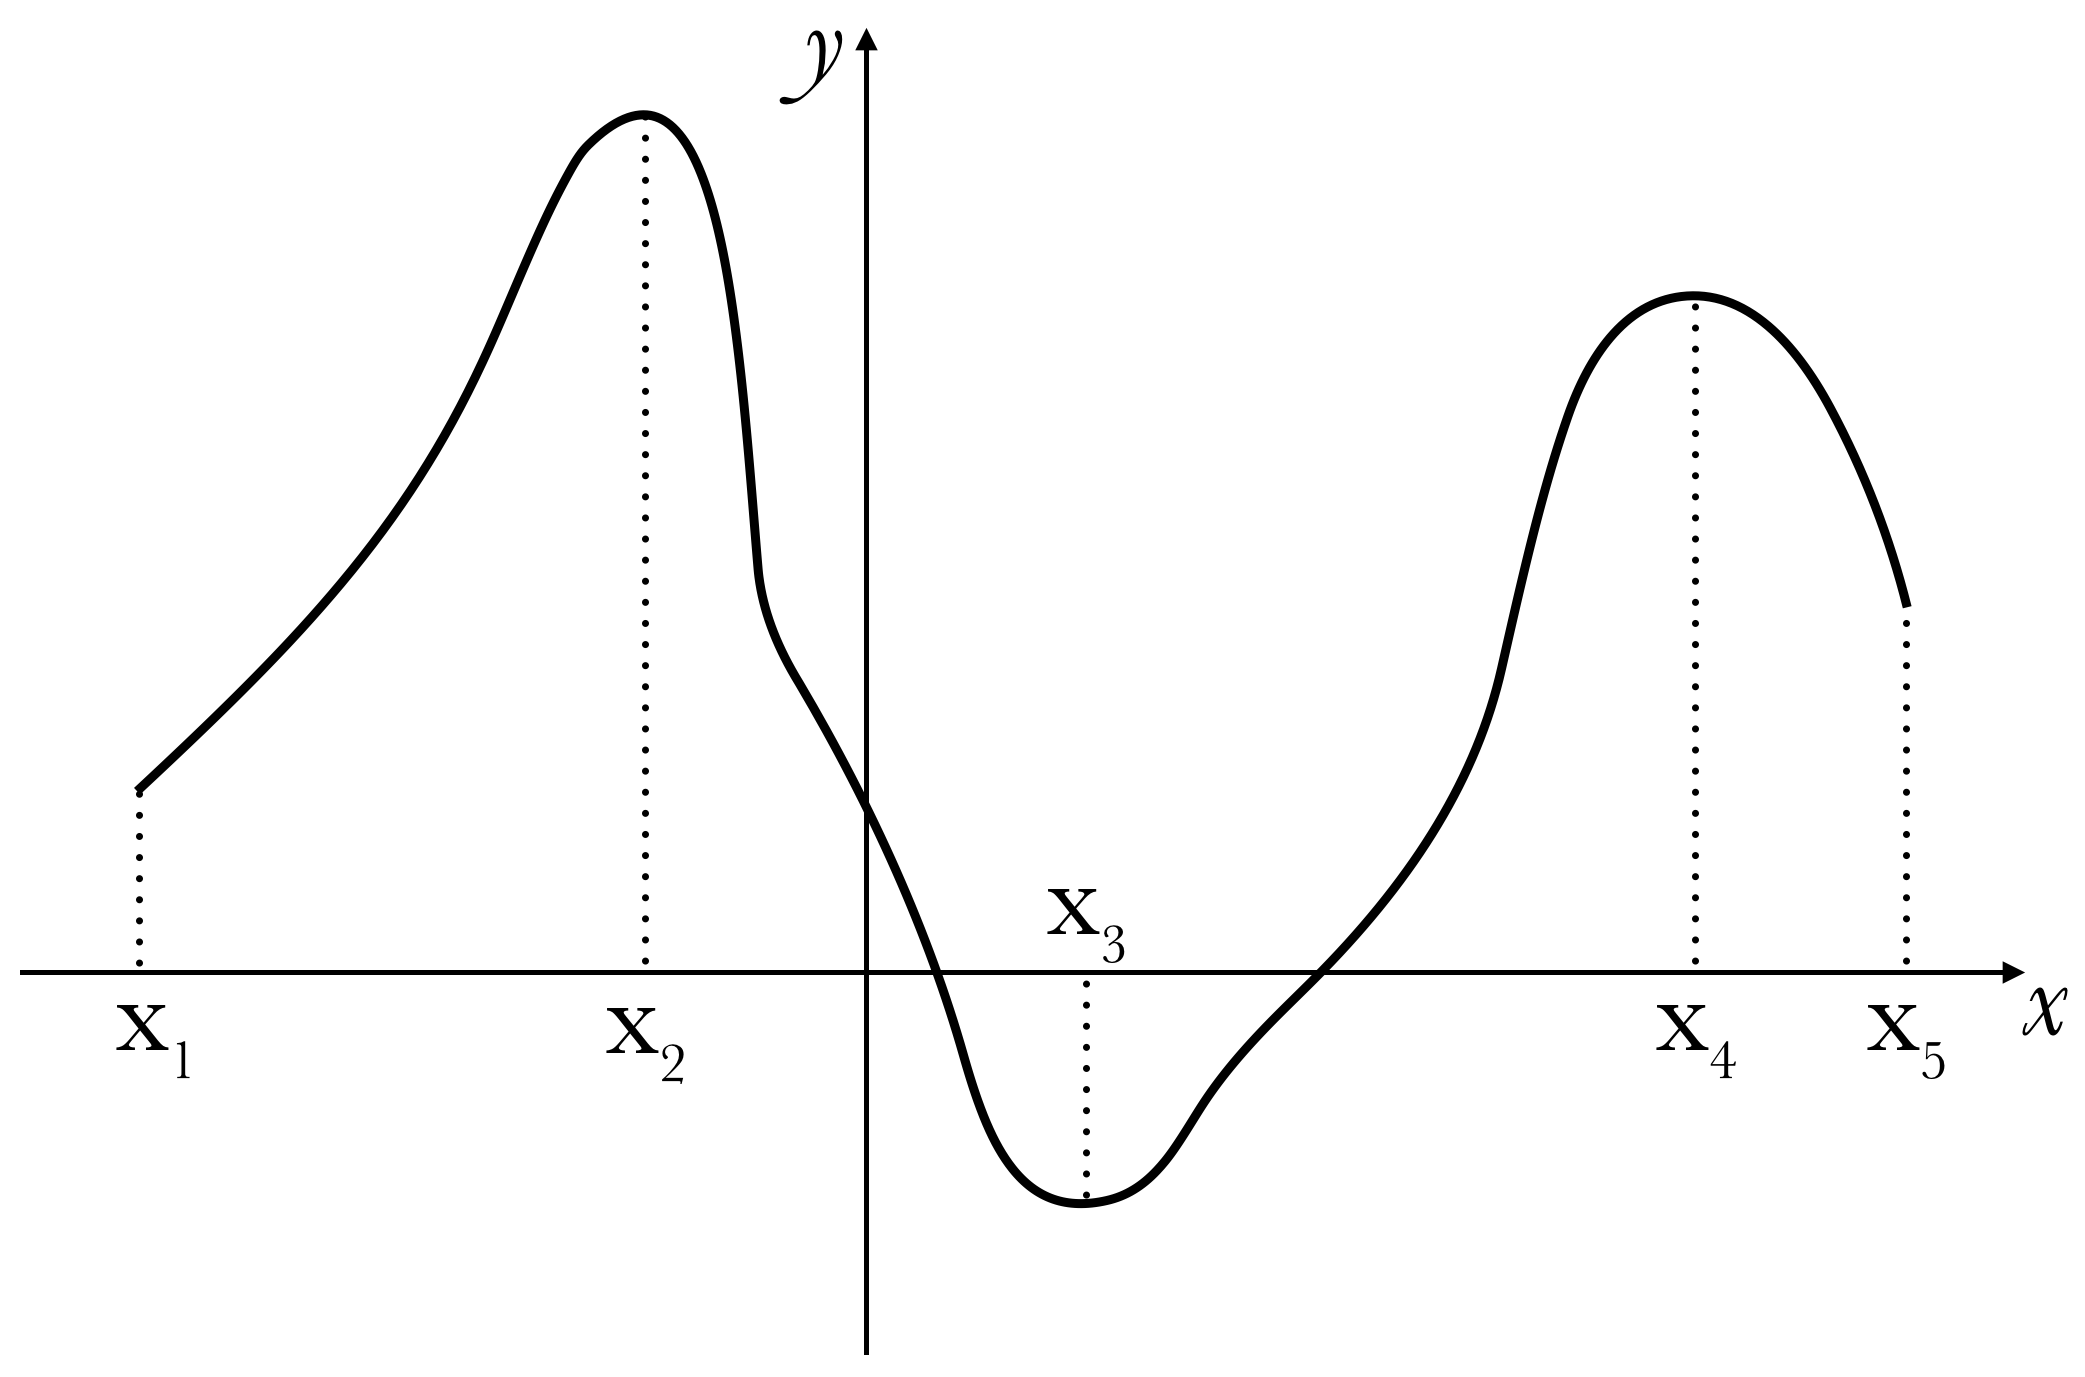
\includegraphics[width=0.4\textwidth]{img/funz_8.png}
  %\caption{}
  %\label{fig:1_2}
\end{figure}
\end{esempio}
\subsection{Parità}
%label{}
La caratteristica della parità va a verificare se il grafico della funzione 
che stiamo studiando è simmetrico rispetto all'asse delle $Y$, cioè il 
grafico è speculare rispetto all'asse, o se il grafico della funzione è 
simmetrico rispetto all'origine. Nel primo caso parleremo di \textsc{parità} 
della funzione, nel secondo caso parleremo di \textsc{disparità} della 
funzione.\\

Ovviamente non tutte le funzioni presenteranno questa simmetria, possiamo 
però individuare delle condizioni che, se presenti nella funzione, ci 
assicurano che questa è pari o dispari.\\

\begin{definizione}
Sia data una funzione $y=f(x)$, avente dominio $D$ tale che per ogni $x\in D$ 
anche $-x\in D$. Una funzione si dice \textsc{pari} in $D$ se \\
$$f(-x)=f(x)$$
per ogni $x\in D$.
\end{definizione}

\begin{figure}[htpb!]
  \centering
  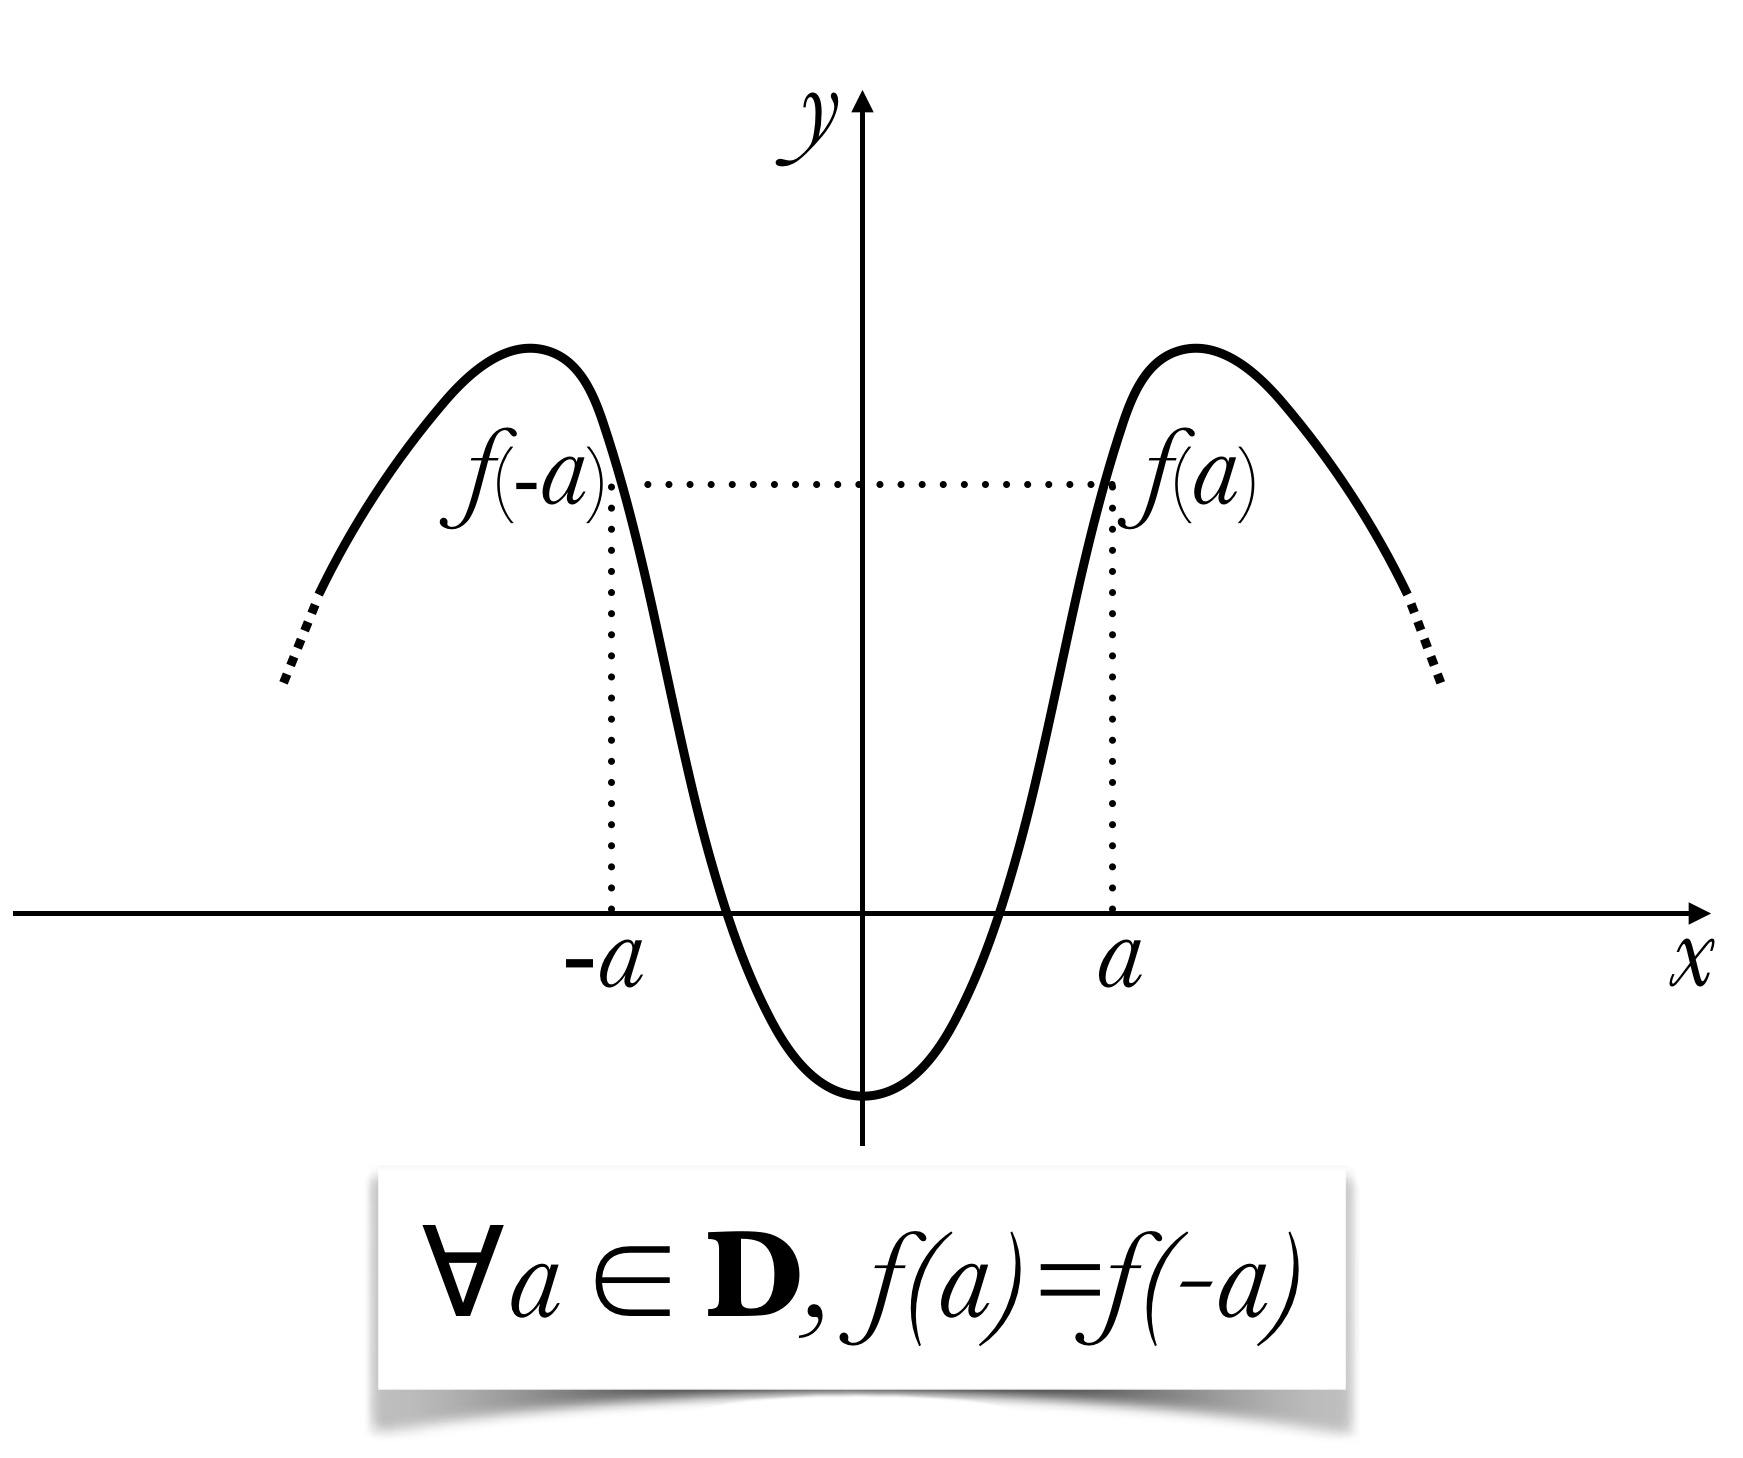
\includegraphics[width=0.5\textwidth]{img/funz_9.png}
  %\caption{}
  %\label{fig:1_2}
\end{figure}
%

Se una funzione è pari, il suo grafico è simmetrico rispetto all'asse $Y$. 
Infatti se $P(x;y)$ appartiene al grafico anche $P'(-x;y)$ vi appartiene. 
Sottolineiamo ancora che la condizione di parità per una funzione è $f(-x)= 
f(x)$.\\   

\begin{esempio} Verificare se una funzione è o non è pari.\\
Per verificare se una funzione è pari basta sostituire nella funzione $-x$ al 
posto di $x$ e verificare se la nuova $f(-x)$ è uguale alla funzione di 
partenza, cioè se $f(-x)=f(x)$. Se prendiamo la funzione 
$$f(x)=\frac{x^2+3}{x+2}$$ \underline{non} è pari, infatti 
$$f(-x)=\frac{(-x)^2+3}{(-x)+2}=\frac{x^2+3}{-x+2}\neq f(x).$$
\end{esempio}

\begin{definizione}
Sia data una funzione $y=f(x)$, avente dominio $D$ tale che per ogni $x\in D$ 
anche$ -x\in D.$ Una funzione si dice \textsc{dispari} in $D$ se\\
$$f(-x)=-f(x)$$
per ogni $x\in D$.
\end{definizione}

\begin{figure}[htpb!]
  \centering
  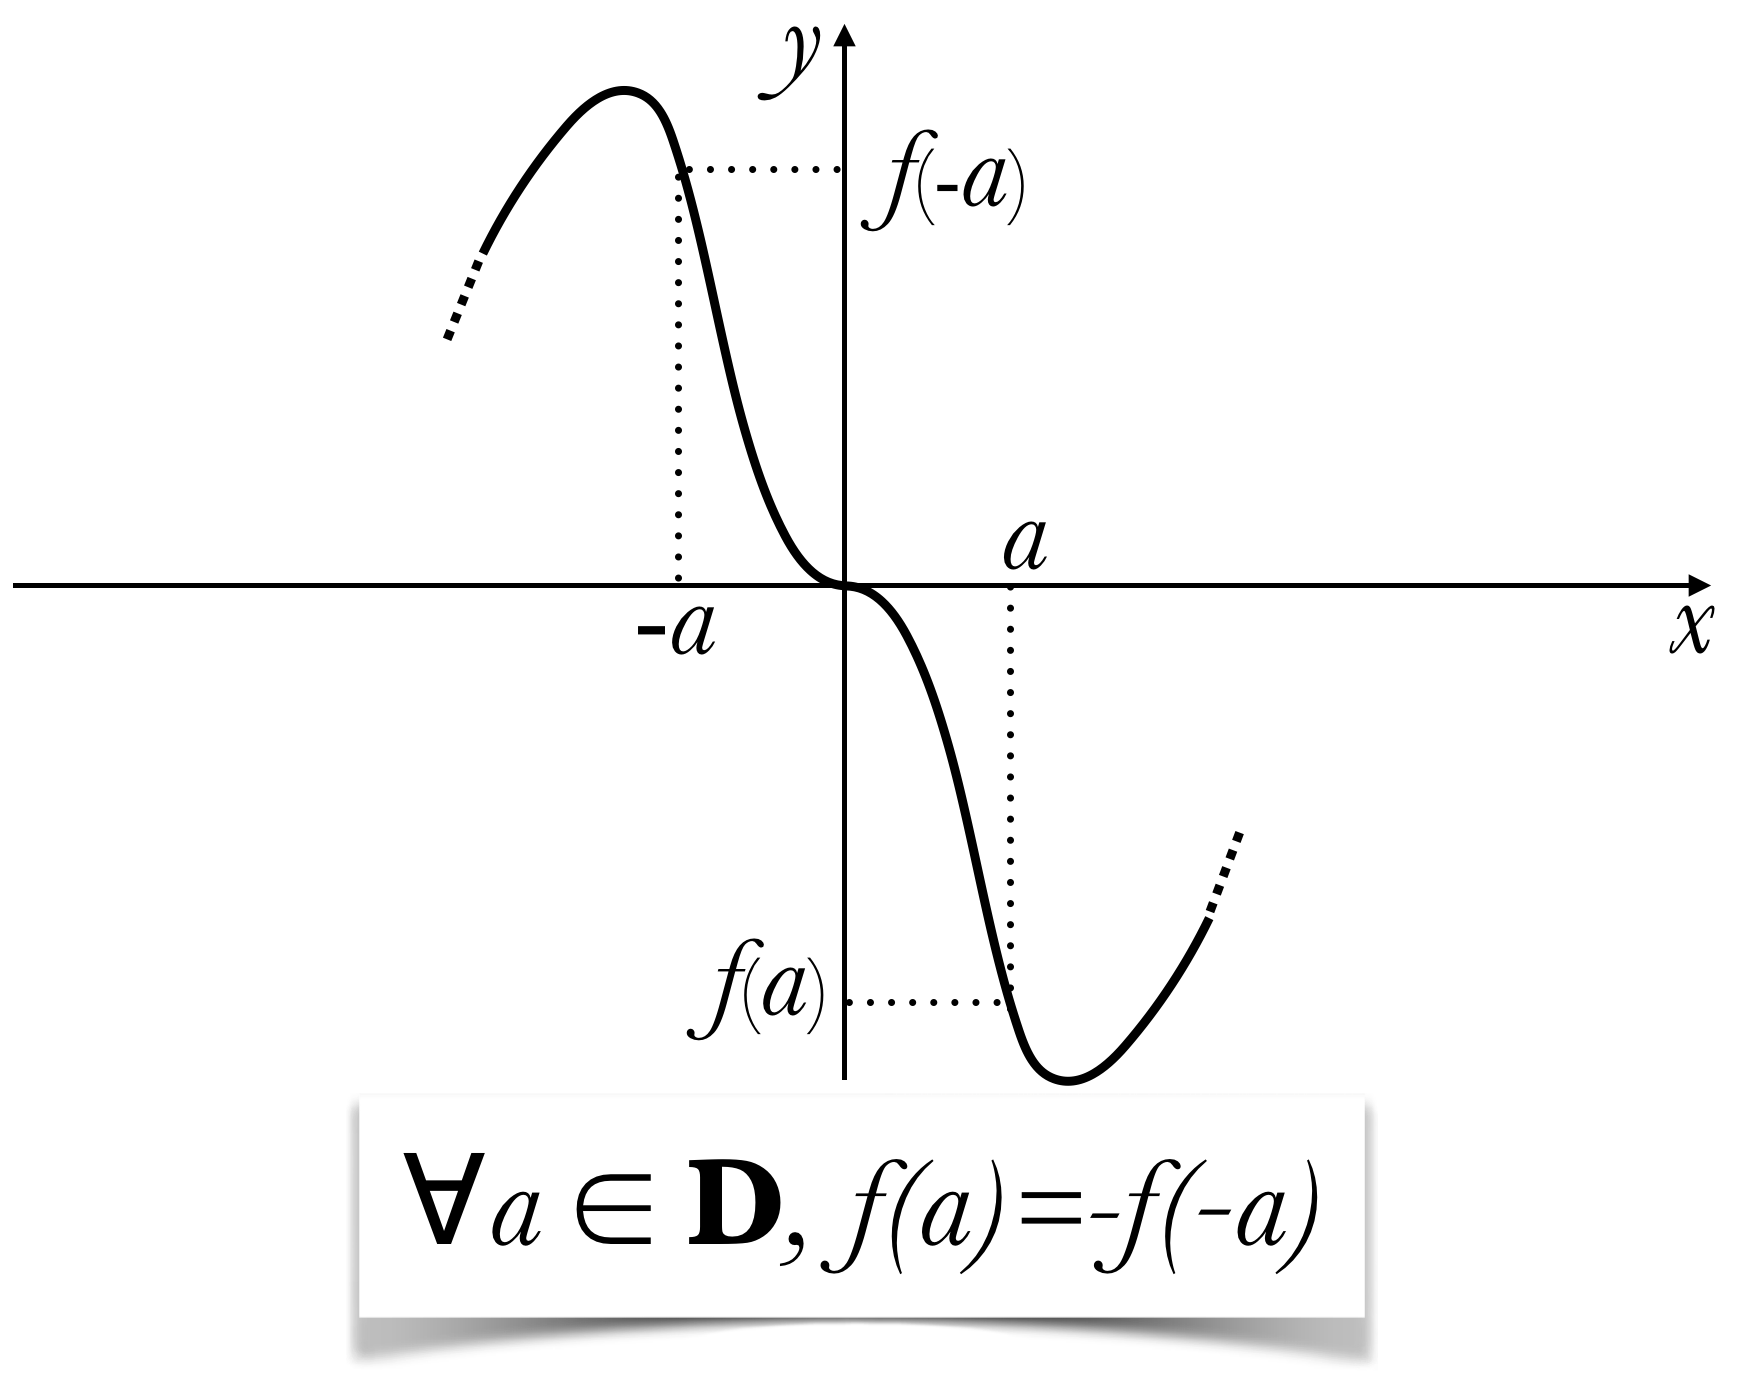
\includegraphics[width=0.5\textwidth]{img/funz_10.png}
  %\caption{}
  %\label{fig:1_2}
\end{figure}
%

Se una funzione è dispari, il suo grafico è simmetrico rispetto all'origine. 
Infatti se $P(x;y)$ appartiene al grafico anche $P'(-x;-y)$ vi appartiene. 
Sottolineiamo ancora che la condizione di disparità per una funzione è 
$f(-x)= -f(x)$. \\

\begin{esempio} Verificare se una funzione è o non è dispari.\\
Per verificare se una funzione è dispari basta sostituire nella funzione $-x$ 
al posto di $x$ e verificare se la nuova $f(-x)$ è uguale alla funzione di 
partenza cambiata di segno, cioè se $f(-x)=-f(x)$. Se prendiamo la funzione 
$$f(x)=\frac{x}{x^2+2}$$ è dispari, infatti 
$$f(-x)=\frac{(-x)}{(-x)^2+2}=\frac{-x}{x^2+2}=-\frac{x}{x^2+2}= -f(x).$$
\end{esempio}

\subsection{Periodicità}
%label{}
La periodicità di una funzione specifica se questa si ripete uguale a sé 
stessa ad intervalli regolari.\\

\begin{definizione}
Una funzione $y=f(x)$, $f(x): A\to \mathbb{R}$ si dice \textsc{periodica} di 
periodo $T>0$ di periodo $T>0$ se$\forall x\in A\rightarrow (x+T)\in A$e 
possiamo scrivere 
 $$f(x+T)=f(x)$$\\
\end{definizione}

\begin{figure}[htpb!]
  \centering
  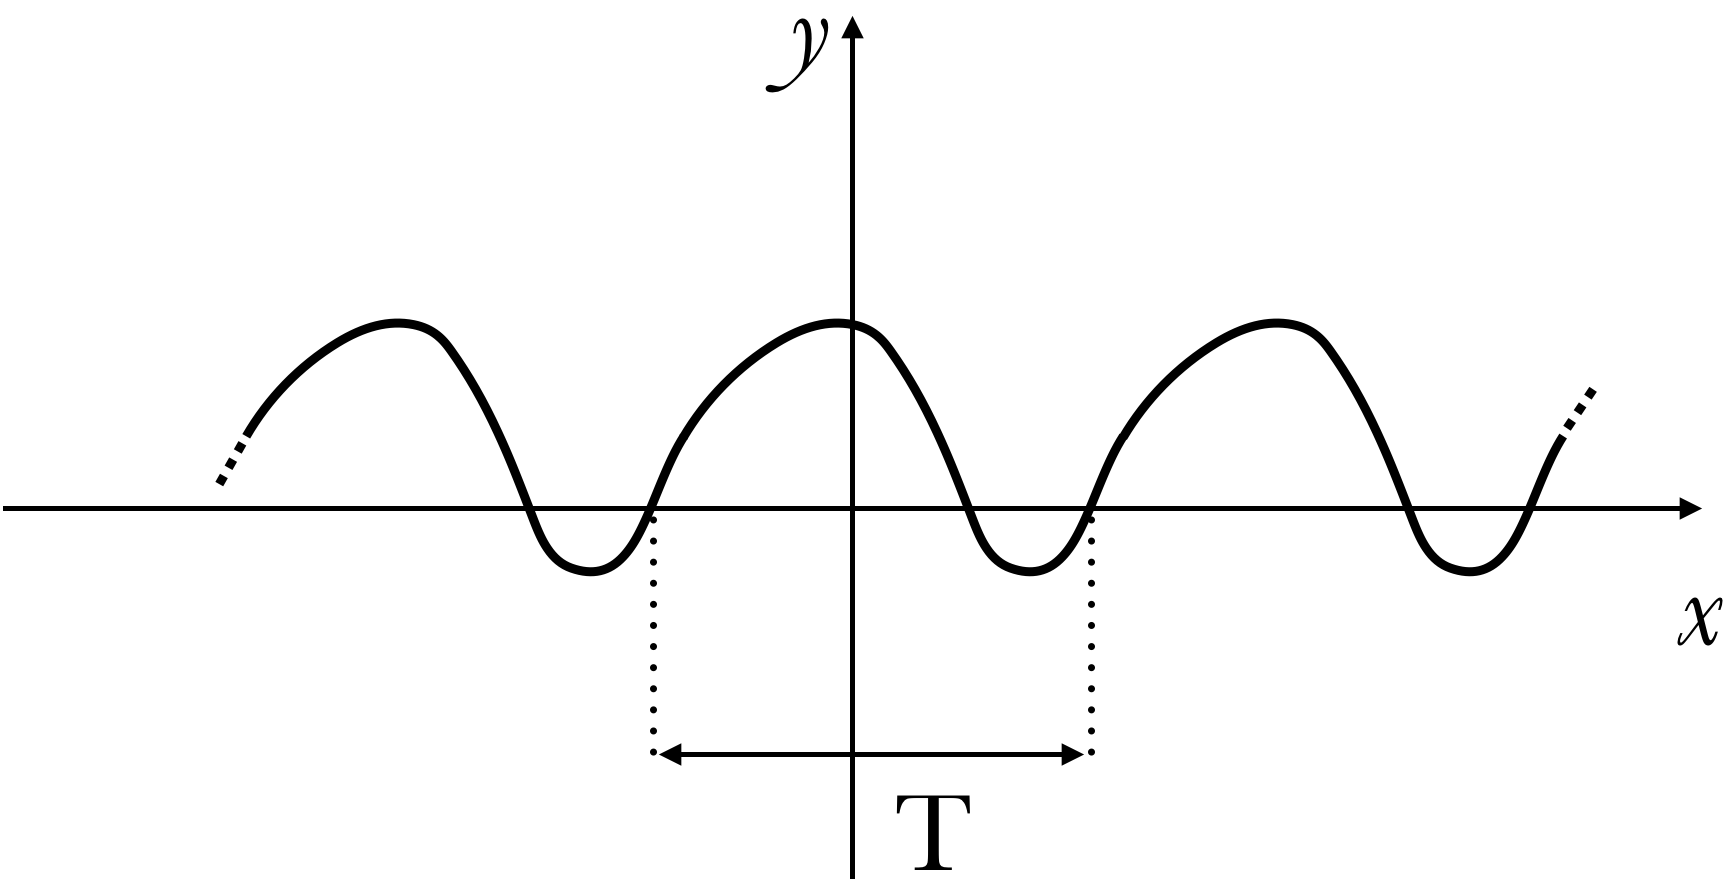
\includegraphics[width=0.45\textwidth]{img/funz_11a.png} \quad 
  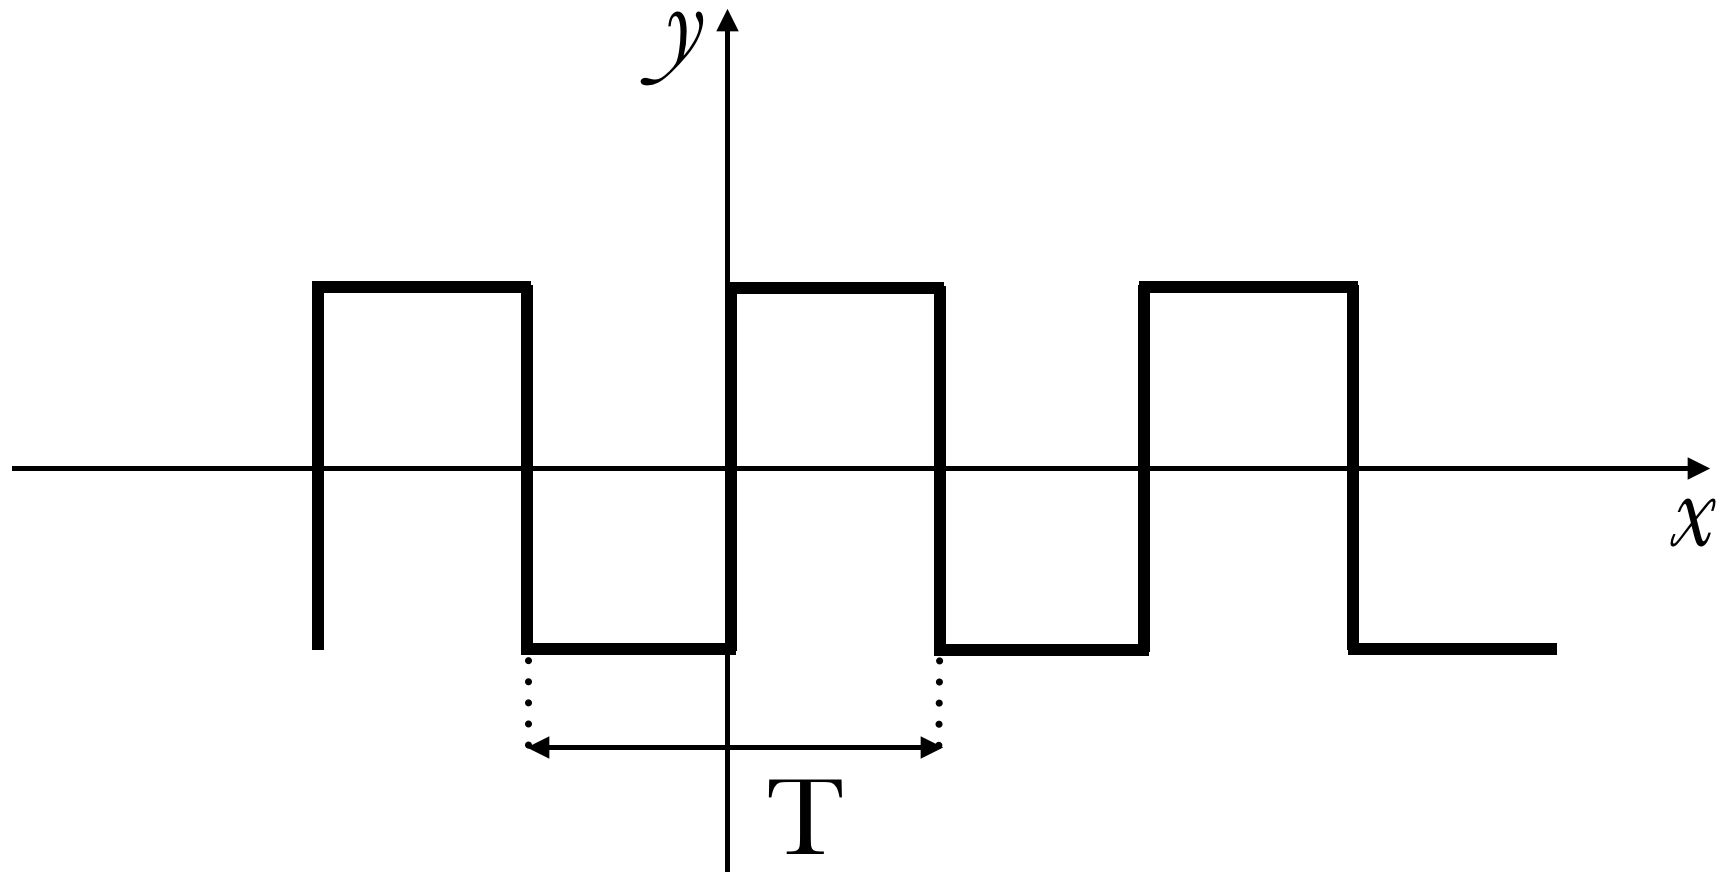
\includegraphics[width=0.45\textwidth]{img/funz_11b.png}
  %\caption{}
  %\label{fig:1_2}
\end{figure}


\begin{esempio} Calcolare il periodo di una funzione.\\
Calcoliamo il periodo della  funzione goniometrica $$y=\sin{7x}$$ con due 
possibili procedure:
\begin{itemize}
  \item[\textsf{Procedura a)}] La funzione ha per definizione periodo 
$T$ se, con $k$ intero,
$$\sin[(7(x+kT)]=\sin4x$$
cioè,
$$\sin[(7x+7kT)]=\sin4x$$
poichè la funzione seno ha periodo $2\pi$, allora
$$\sin[7x+7kT]=\sin[7x+2k\pi]$$
e l'uguaglianza è quindi valida se $7T=2\pi$ da cui
$$T=\frac{2\pi}{7}.$$

  \item[\textsf{Procedura b)}] La funzione $y'=\sin7x'$ viene dalla 
trasformazione della funzione $y=\sin x$, che ha periodo $T=2\pi$, mediante 
una sostituzione $7x'=x$, ovvero $x'=\frac{x}{7}$. Se l'asse delle ascisse 
viene così contratto di un fattore $\frac{x}{7}$, il periodo $T'$ subirà la 
stessa contrazione e pertanto è pari a $$T'=\frac{x}{7}(2\pi)=\frac{2\pi}{7}$$
\end{itemize}
\end{esempio}

Se due funzioni $f(x)$ e $g(x)$ hanno periodi diversi $T_f$ e $T_g$, 
rispettivamente, le funzioni $f(x)\pm g(x)$, $f(x)\cdot g(x)$ e 
$\frac{f(x)}{g(x)}$ hanno un periodo pari al m.c.m. tra $T_f$ e $T_g$ 
nell'ipotesi che $\frac{T_f}{T_g}$ sia un numero razionale e diverso da 1. Se 
il rapporto è irrazionale le precedenti combinazioni di funzioni non sono 
periodiche. Se $T_f=T_g$ il periodo globale è minore o uguale del periodo 
comune.\\

\begin{esempio} Calcolare il periodo di combinazioni di funzioni periodiche e 
non periodiche.\\
  \begin{itemize}
  \item[a)] $f(x)=\sin x+\cos 3x$ è periodica di $2\pi$ che è 
il m.c.m. tra $T_f=2\pi$ e $T_g=\frac{2}{3}\pi$.
  
  \item[b)] $f(x)=\sin x+\cos \pi x$ non è periodica perché il 
rapporto $\frac{T_f}{T_g}\notin \mathbb{Q}$, infatti $T_f=2\pi$ e $T_g=2$, 
per cui $\frac{2\pi}{2}=\pi\notin\mathbb{Q}$
  
  \item[c)] $f(x)=\sin \frac{x}{2}-\cos 3x+\tan x$ dove 
$T_{\sin \frac{x}{2}}=4\pi$, $T_{\cos 3x}=\frac{2}{3}\pi$, $T_{\tan}=\pi$
  
  \item[d)] Se consideriamo la funzione 
$$f(x)=\frac{1}{\log[\sin x]}$$ il periodo è $2\pi$
\end{itemize}
\end{esempio}

Se una funzione è periodica i valori delle sue ordinate si ripetono con 
regolarità, quindi per studiarne l'andamento su tutto l'asse reale, basterà 
studiarne l'andamento in un singolo periodo. Ripetiamo ancora che la 
condizione di parità per una funzione è $f(x+T)=f(x)$ con $T$ periodo.
%
%
\subsection{Limitatezza}
%label{}
La limitatezza di una funzione valuta se le ordinate di una funzione 
raggiungono un valore massimo e un valore minimo, oppure non hanno un 
limite.\\


\begin{definizione}
Consideriamo una funzione $f: A\to \mathbb{R}$, la funzione si dice:
  \begin{itemize}
  \item[$\rhd$]\textsc{limitata superiormente} se il suo 
codominio $f(A)$ ha un limite superiore $k$:
$$\exists k\in \mathbb{R} \vert \forall x\in A,\, k\geq f(x)$$ 
  \item[$\rhd$]\textsc{limitata inferiormente} se il suo 
codominio f(A) ha un limite inferiore $k$: 
$$\exists k\in \mathbb{R} \vert \forall x\in A,\, k\leq f(x)$$

  \item[$\rhd$]\textsc{limitata} se il suo codominio $f(A)$ è 
limitato sia superiormente che inferiormente:
$$\exists k\in \mathbb{R},k>0\vert\forall x\in A, \vert f(x)\vert \leq k$$
\end{itemize}

Se una funzione non è limitata da un valore del codominio $k$ si dirà 
illimitata, in particolare:
  \begin{itemize} 
  \item[$\rhd$] \textsc{Illimitata superiormente} se il suo 
codominio $f(A)$ \underline{non} è limitato superiormente;
  \item[$\rhd$] \textsc{Illimitata inferiormente} se il suo 
codominio $f(A)$ \underline{non} è limitato inferiormente;
  \item[$\rhd$] \textsc{Illimitata} se il suo codominio $f(A)$ 
\underline{non} è limitato superiormente \underline{né} inferiormente.
  \end{itemize}
\end{definizione}
%
\begin{esempio} Determinare la limitatezza o illimitatezza di funzioni.\\
In (a) La funzione $f(x)=\log(x)$ è illimitata: né superioremente né 
inferiormente limitata; in (b) La funzione è limitata inferiormente e 
illimitata superiormente; in (c) La funzione $f(x)=\sin{x}$ è limitata sia 
superiormente che inferiormente; in (d) La funzione $f(x)=x^2$ è limitata 
inferiormente e illimitata superiormente.
\begin{figure}[h]
  \centering
  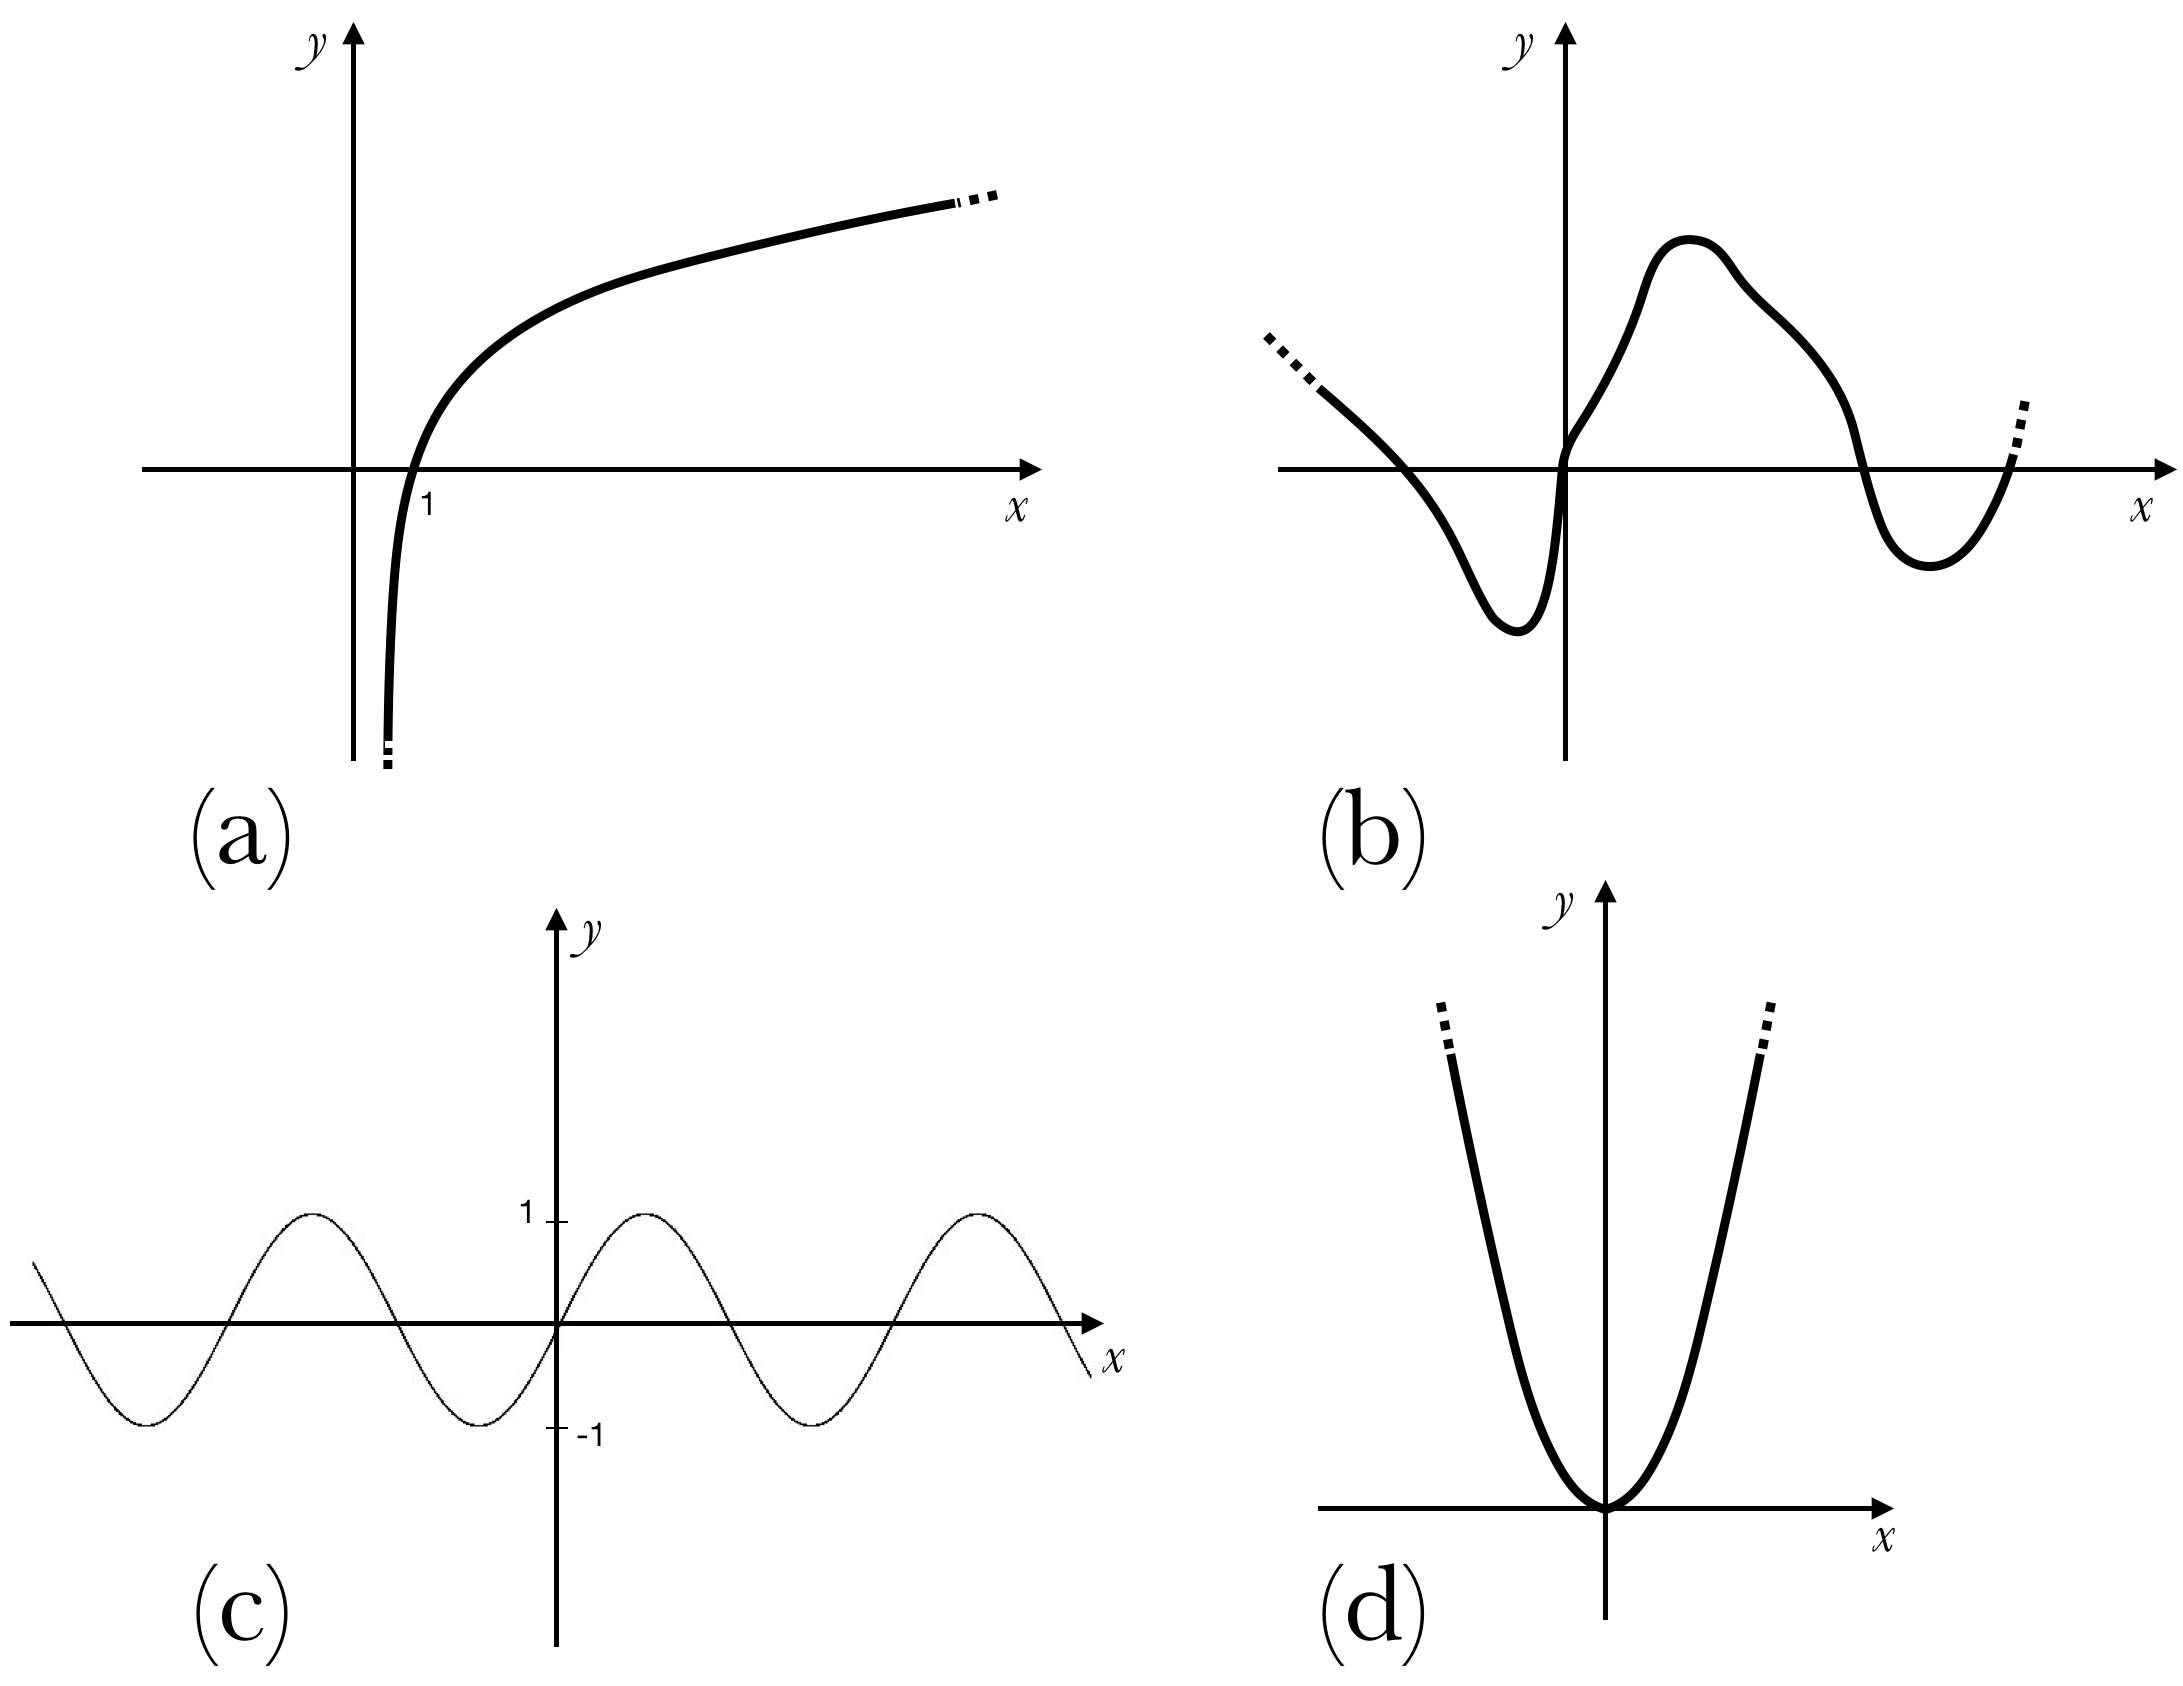
\includegraphics[width=0.85\textwidth]{img/funz_12a.png}
  %\label{fig:1_2}
\end{figure}
\end{esempio}
\newpage
\section{La classificazione delle funzioni}
%label{}
Classifichiamo le possibili funzioni che incontreremo o abbiamo incontrato in 
base alle operazioni che compaiono nella loro espressione analitica. Se 
nell'espressione analitica di una funzione compaiono le operazioni di 
addizione, sottrazione, moltiplicazione, divisione, elevamento a potenza con 
esponente razionale o estrazione di radice siamo di fronte ad una 
\textsc{funzione algebrica}.\\

Le funzioni che non possono essere rappresentate usando solamente le 
operazioni precedentemente ricordate si dicono \textsc{trascendenti}. Tra le 
più note funzioni trascendenti ricordiamo le funzioni goniometriche, quelle 
esponenziali e quelle logaritmiche.\\

A seconda che le funzioni algebriche contengano o meno l'operazione di radice 
e l'operazione di divisione suddividiamo le funzioni algebriche in 
\textsc{razionali fratte}, \textsc{razionali intere} o polinomiali, 
\textsc{irrazionali fratte} e \textsc{irrazionali intere}. \\

\textsf{MEMO!!} Per non creare equivoci ricordiamo che una funzione è 
definita fratta quando il denominatore contiene la variabile indipendente 
$x$, è invece definita irrazionale quando tale variabile appare sotto il 
segno di radice.\\

% TODO non compila!!!!!!!!!!!!!!!!!!!!!!!!!!!!!!!!!!!!!!!!!!!!!!!!!!!
% \Tree [.FUNZIONI [.\textbf{algebriche}  [.razionali fratte intere 
% !{\qbalance} ] [.irrazionali fratte intere !{\qbalance} ] ] 
% [.\textbf{trascendenti} goniometriche esponenziali logaritmiche ] ] \\


\begin{esempio} Classificazione di funzioni.\\
Classifichiamo le seguenti funzioni: 
  \begin{itemize}
  \item[a)] $f(x)=\frac{\sqrt{(x+5)}}{3}$ è una funzione 
irrazionale intera, infatti pur avendo un denominatore, questo non contiene 
la variabile indipendente $x$;
  
  \item[b)] $g(x)=e^{\frac{x}{x-1}}$ è una funzione 
trascendente di tipo esponenziale;

  \item[c)] $h(x)=\sqrt{2}x+4x$ è una funzione razionale 
intera, in quanto la radice compare solo nel numero irrazionale  a 
coefficiente della $\sqrt{2}$ $x$.
  \end{itemize}
\end{esempio}

\section{Funzioni inverse, composte e uguali}
%label{}
Nella rappresentazione insiemistica studiata finora abbiamo sempre visto le 
frecce partire dall'insieme $A$ per arrivare nell'insieme $B$. Esiste una 
possibile lettura al contrario? Se le frecce partissero da $B$, dalle $y$ per 
arrivare alle $x$, ci troveremmo ancora in presenza di una funzione?

\begin{definizione}
Sia $f : A\to B$ una funzione biiettiva. Si dice funzione inversa di $f$ la 
funzione $f^{-1} : B\to A$ che associa a ogni $y$ di $B$ il valore $x$ di $A$ 
tale che $y=f(x)$.
\end{definizione}

\begin{figure}[htpb!]
  \centering
  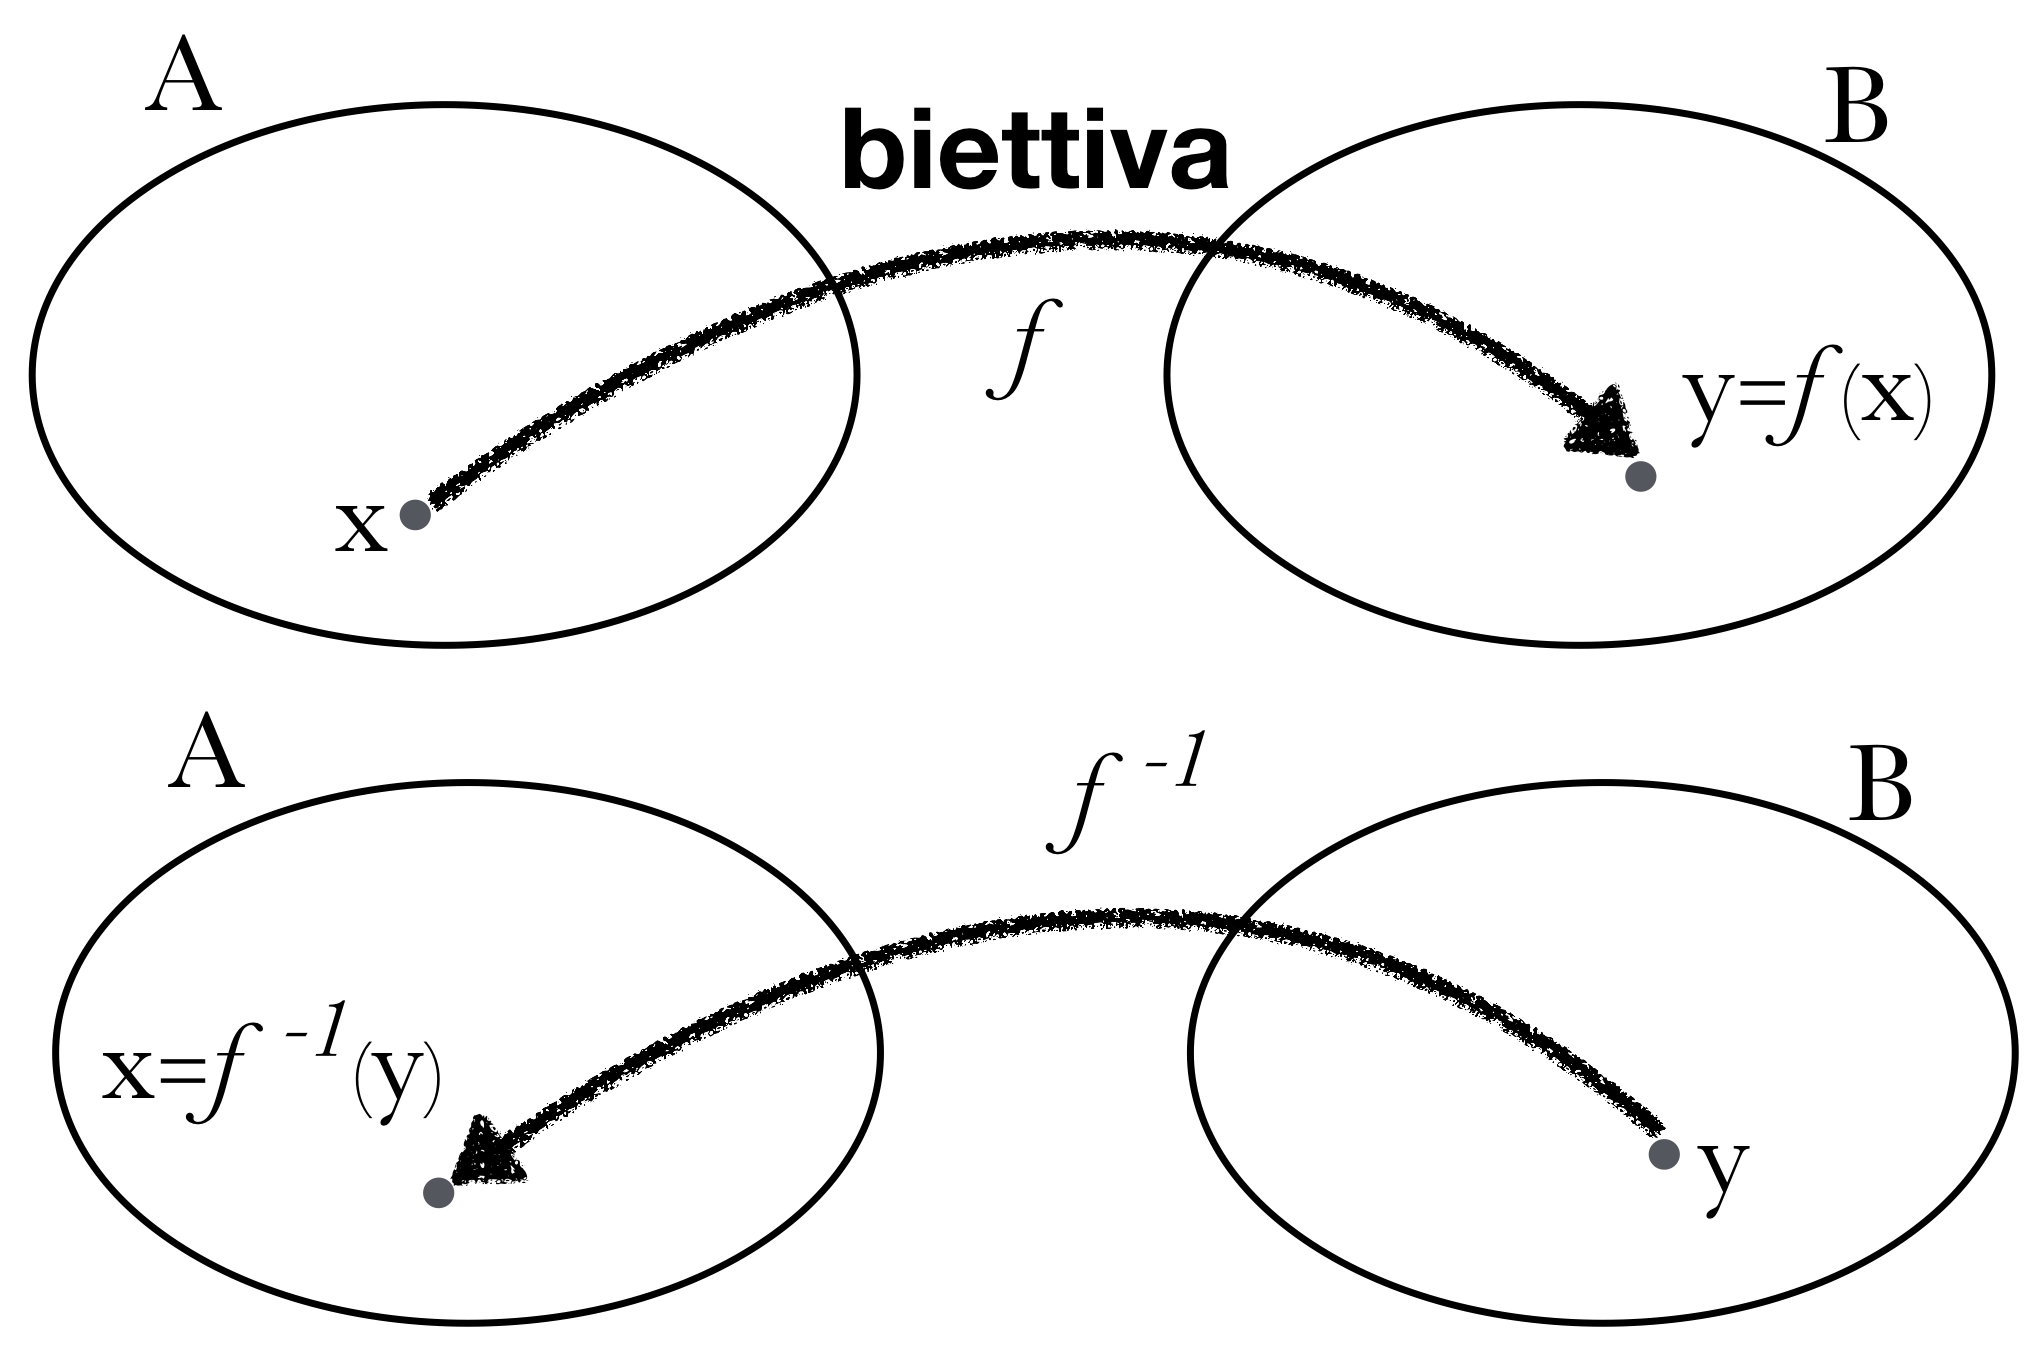
\includegraphics[width=0.45\textwidth]{img/funz_12.png} 
  %\caption{}
  %\label{fig:1_2}
\end{figure}

Notiamo che se una funzione ammette inversa si dice \textsc{invertibile}. 
Significativa è, poi, la relazione tra i codomini e i domini delle due 
funzioni, $f$ e la sua inversa: il dominio di $f^{-1}$ è l'immagine di $f$ e 
l'immagine di $f^{-1}$ è il dominio di $f$.\\

\begin{esempio} Calcolare  e graficare l'inversa di una funzione, verificando 
che sia invertibile.\\ 
Consideriamo la funzione biiettiva $f:\mathbb{R}\to\mathbb{R}$ definita da
$$f(x)=y=3x+2$$
Possiamo ottenere la sua inversa $f^{-1}$ nel seguente modo:
  \begin{itemize}
  \item ricaviamo $x$ in funzione di $y$ dalla relazione 
precedente
$$x=\frac{y-2}{3}$$
  \item sostituiamo la $x$ con $y$ e viceversa.
  \begin{figure}[htpb!]
  \centering
  
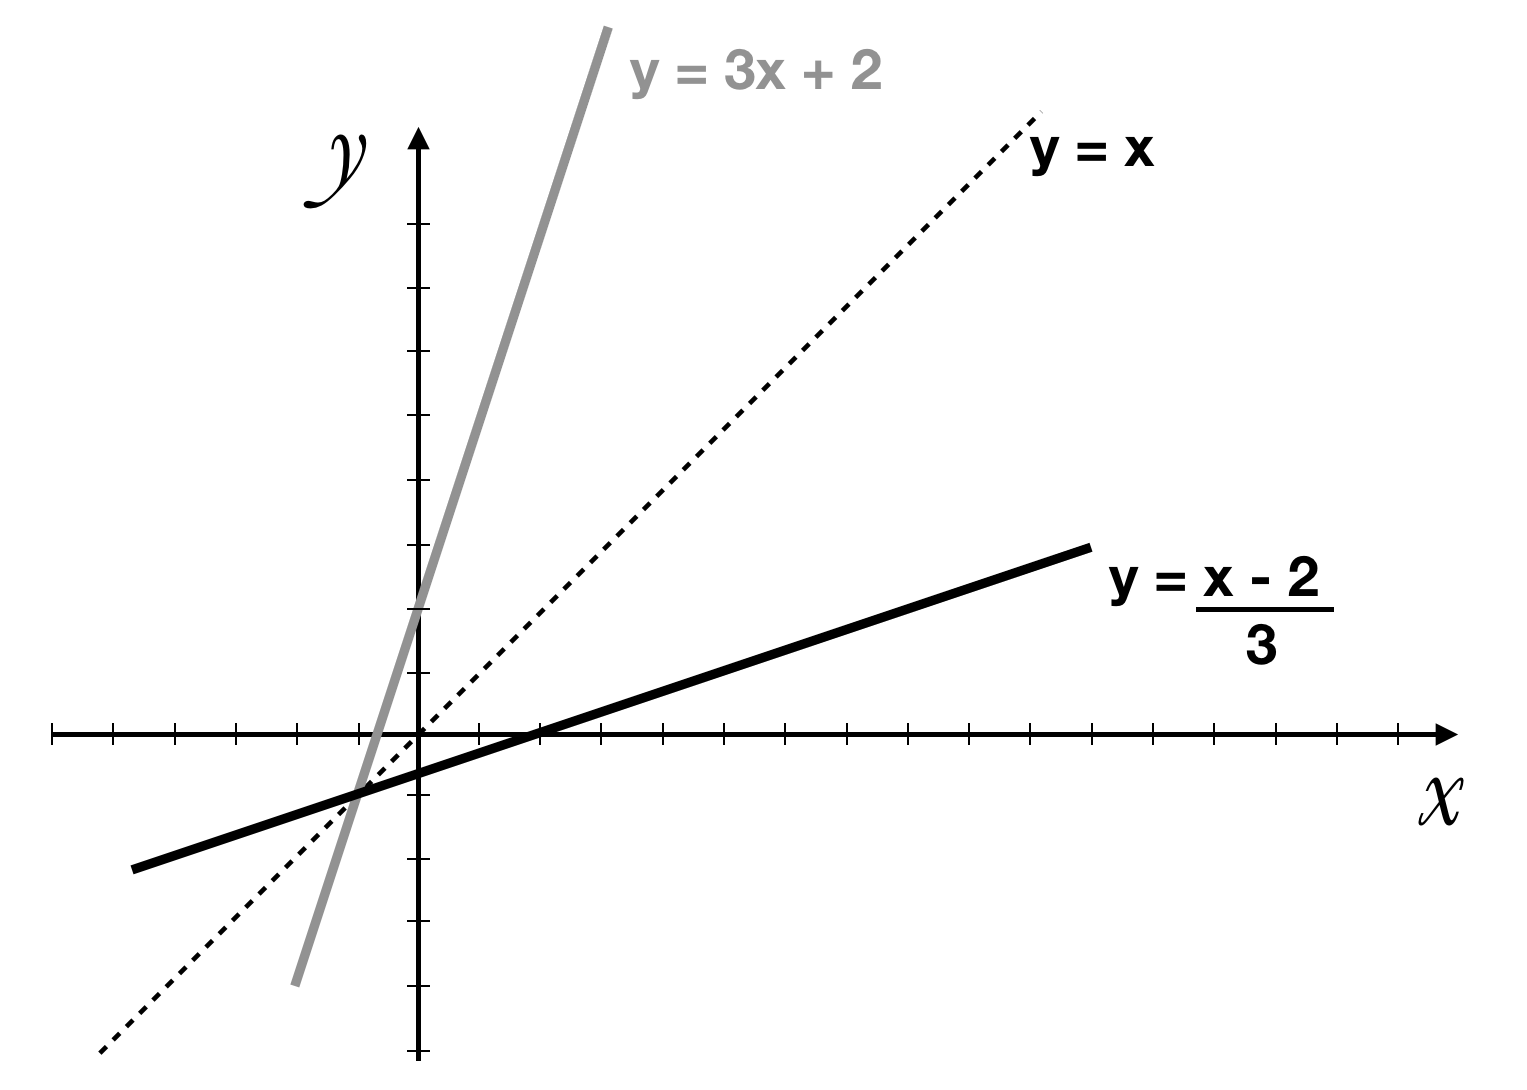
\includegraphics[width=0.5\textwidth]{img/funz_13.png} 
  %\caption{}
  %\label{fig:1_2}
  \end{figure}
  \item notiamo che il grafico della funzione inversa
$$f^{-1}(x)=\frac{x-2}{3}$$
è simmetrico a quello di $f(x)$ rispetto alla bisettrice del primo e terzo 
quadrante, la retta di equazione $y=x$
  \end{itemize}
\end{esempio}

\begin{esempio} Disegnare l'inversa di una funzione che originariamente non 
sia invertibile nel suo dominio. 

La funzione $f:\mathbb{R}\to\mathbb{R}$ tale che $$f(x)=x^2+1$$.
\begin{itemize}
  \item $f$ non ammette funzione inversa perché non è biiettiva, in 
quanto non è iniettiva.
  \begin{figure}[htpb!]
  \centering
  
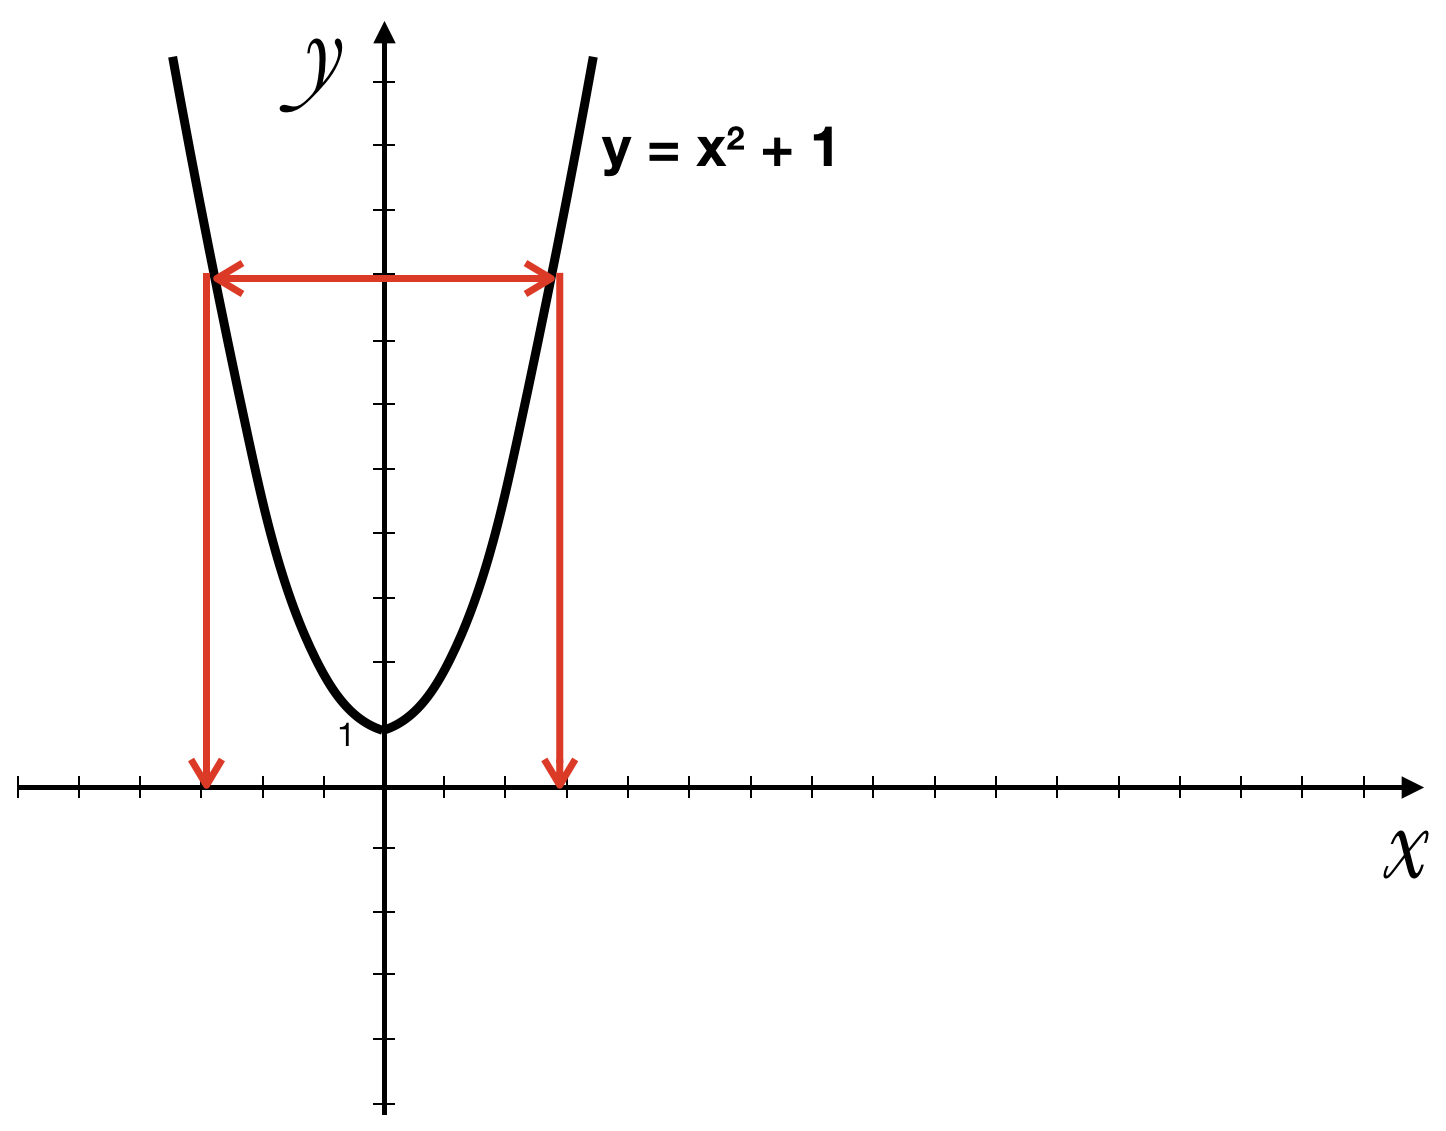
\includegraphics[width=0.45\textwidth]{img/funz_14a.png} %\quad
  
%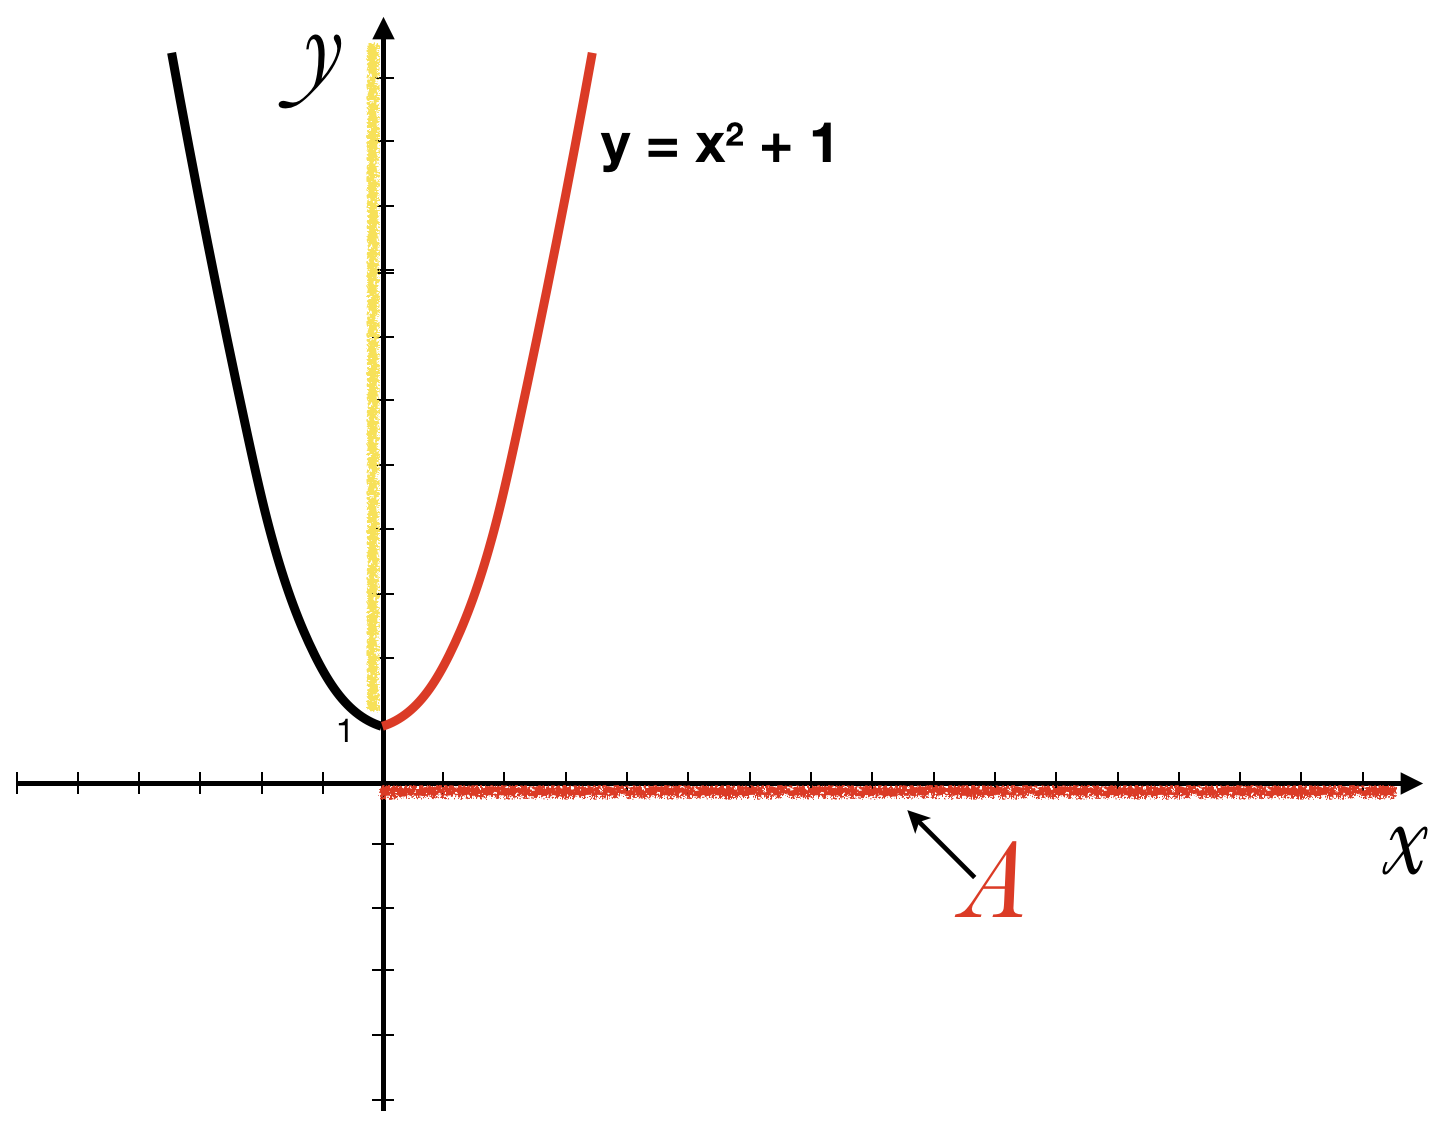
\includegraphics[width=0.7\textwidth]{img/funz_14b.png} \quad
  
%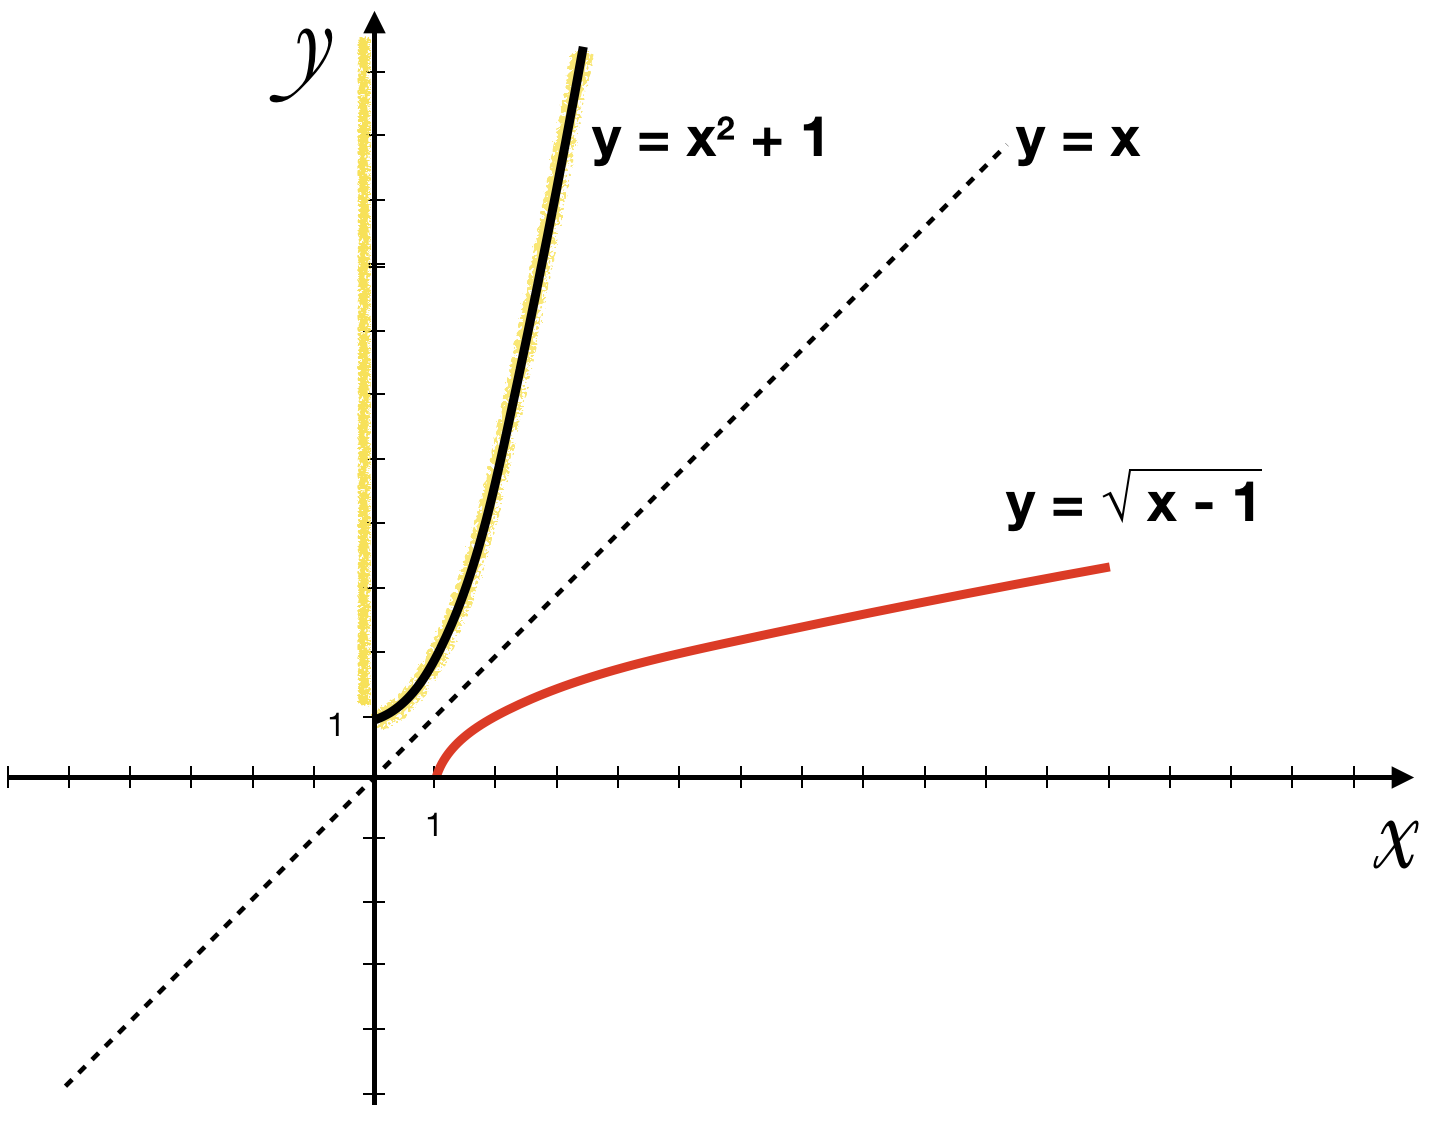
\includegraphics[width=0.7\textwidth]{img/funz_14c.png} 
  %\caption{}
  %\label{fig:funz_14abc}
  \end{figure}
  \item Se $f$ non è biiettiva e quindi non è invertibile, possiamo 
operare una \textsc{restrizione del dominio} a un sottoinsieme in cui $f$ 
risulti biiettiva.
  \begin{figure}[htpb!]
  \centering
  
%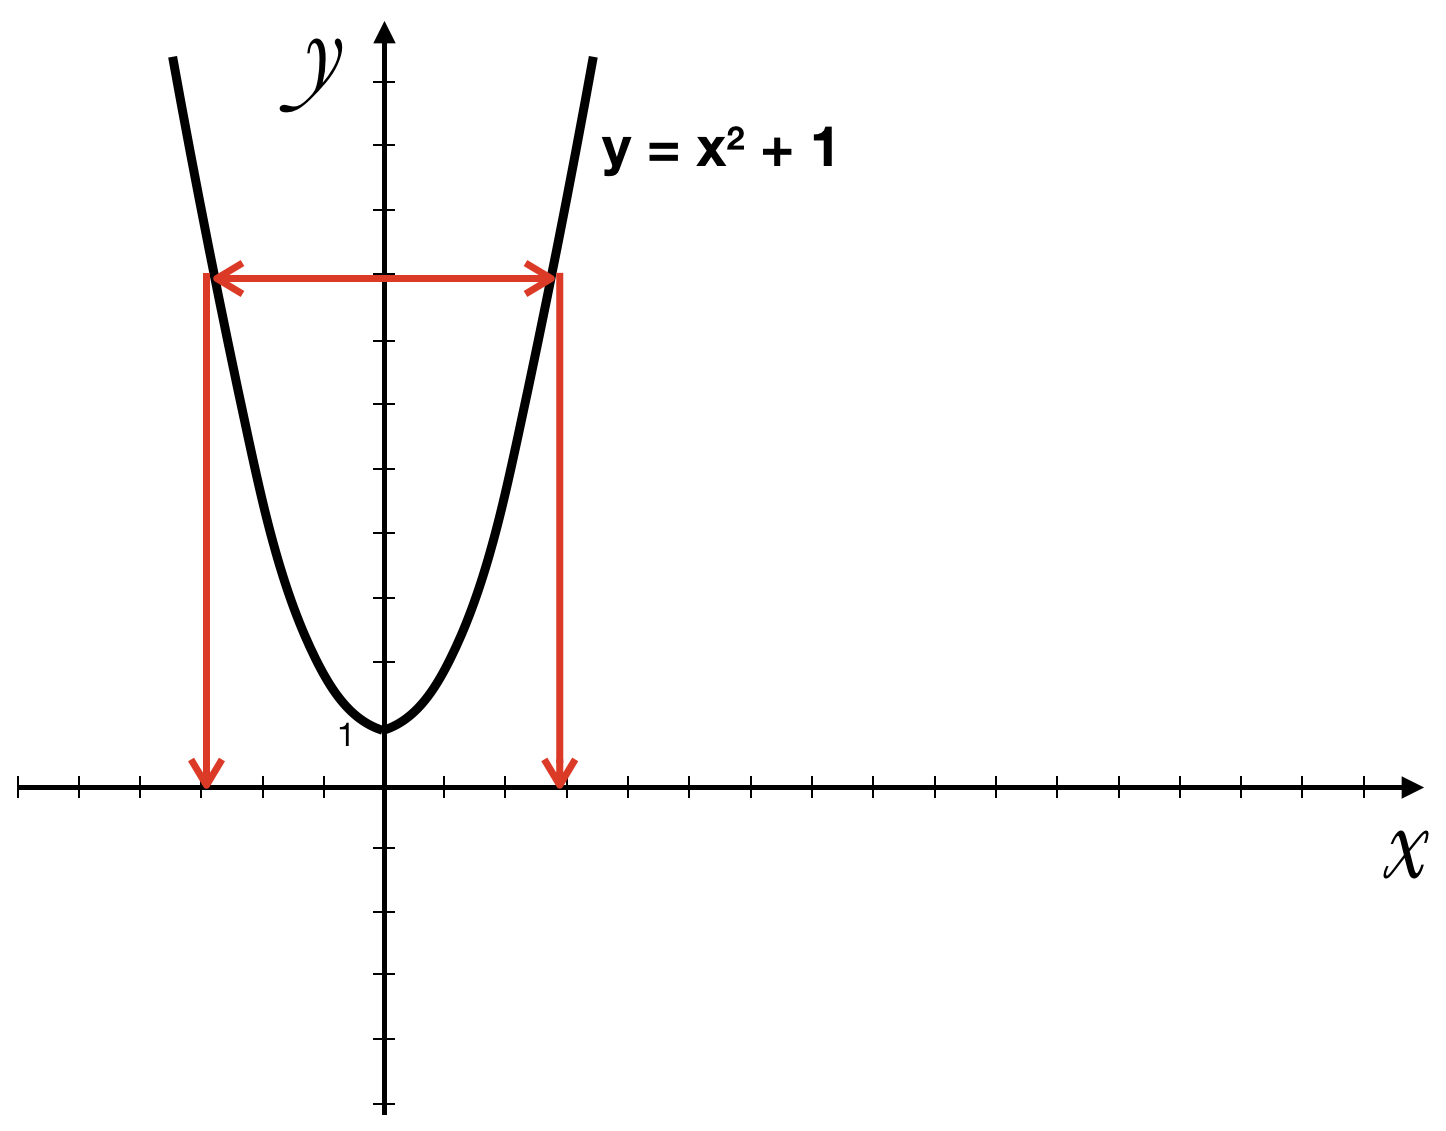
\includegraphics[width=0.7\textwidth]{img/funz_14a.png} %\quad
  
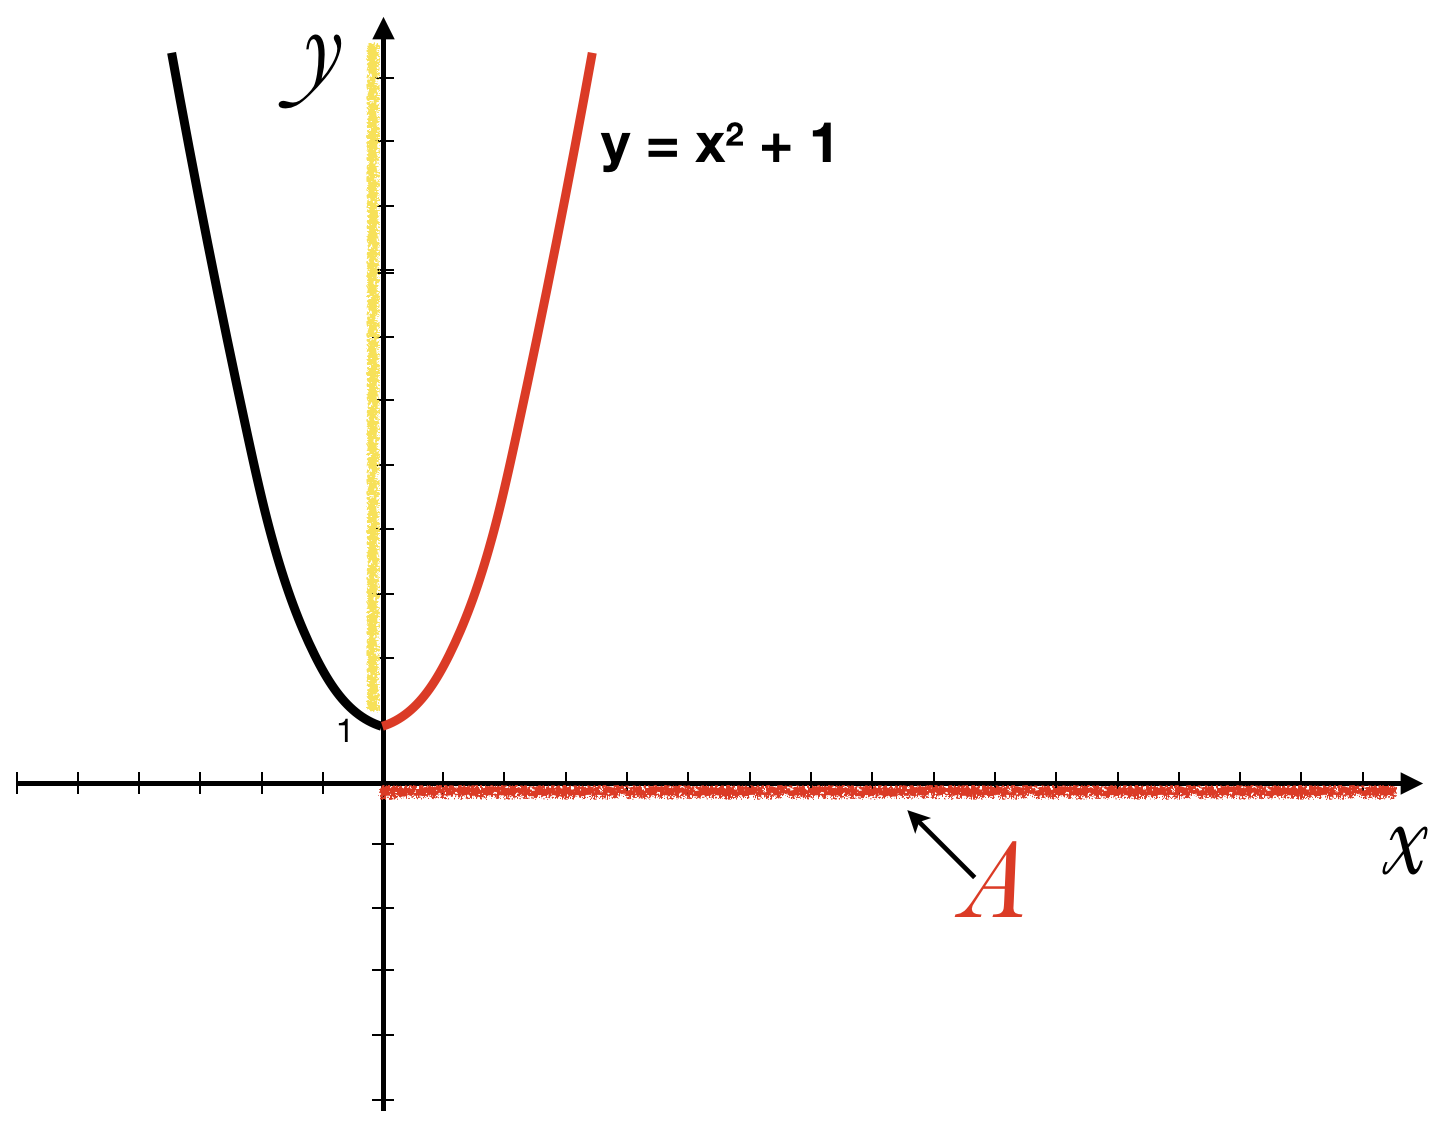
\includegraphics[width=0.45\textwidth]{img/funz_14b.png} %\quad
  
%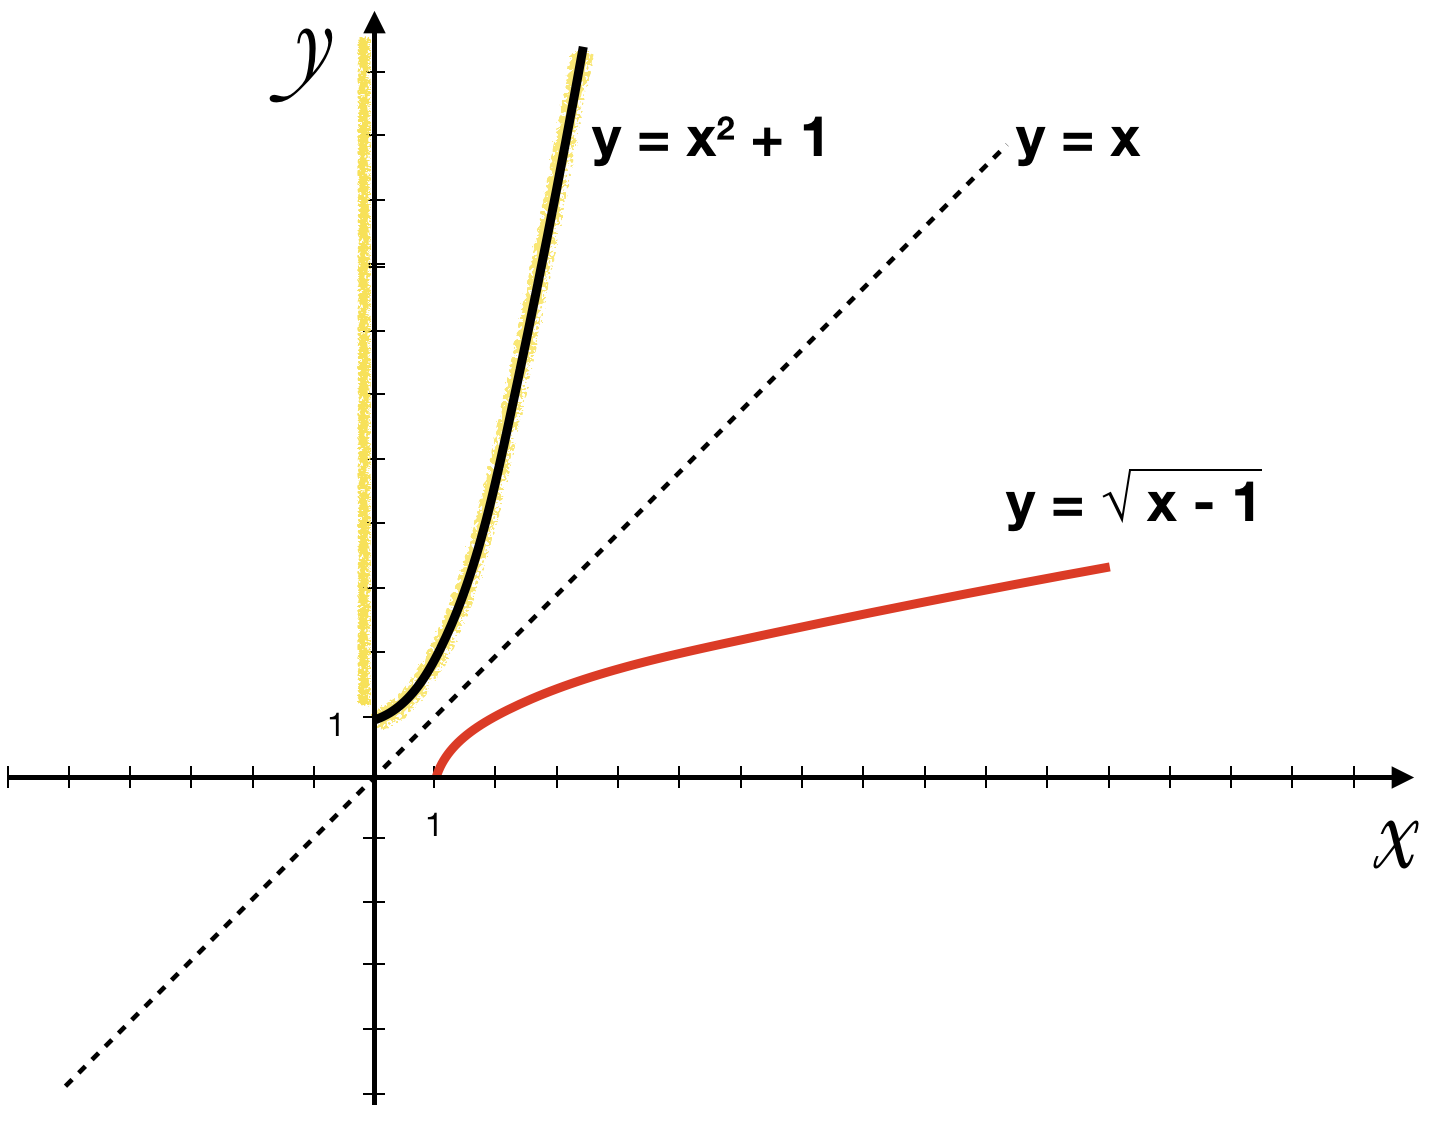
\includegraphics[width=0.7\textwidth]{img/funz_14c.png} 
  %\caption{}
  %\label{fig:funz_14abc}
  \end{figure}
  \item Scelgo solo una parte del dominio che chiamo $A$ e disegno 
l'inversa riflettendo la porzione di funzione biiettiva rispetto alla 
bisettrice del primo e terzo quadrante, la retta di equazione $y=x$.
  \begin{figure}[htpb!]
  \centering
  
%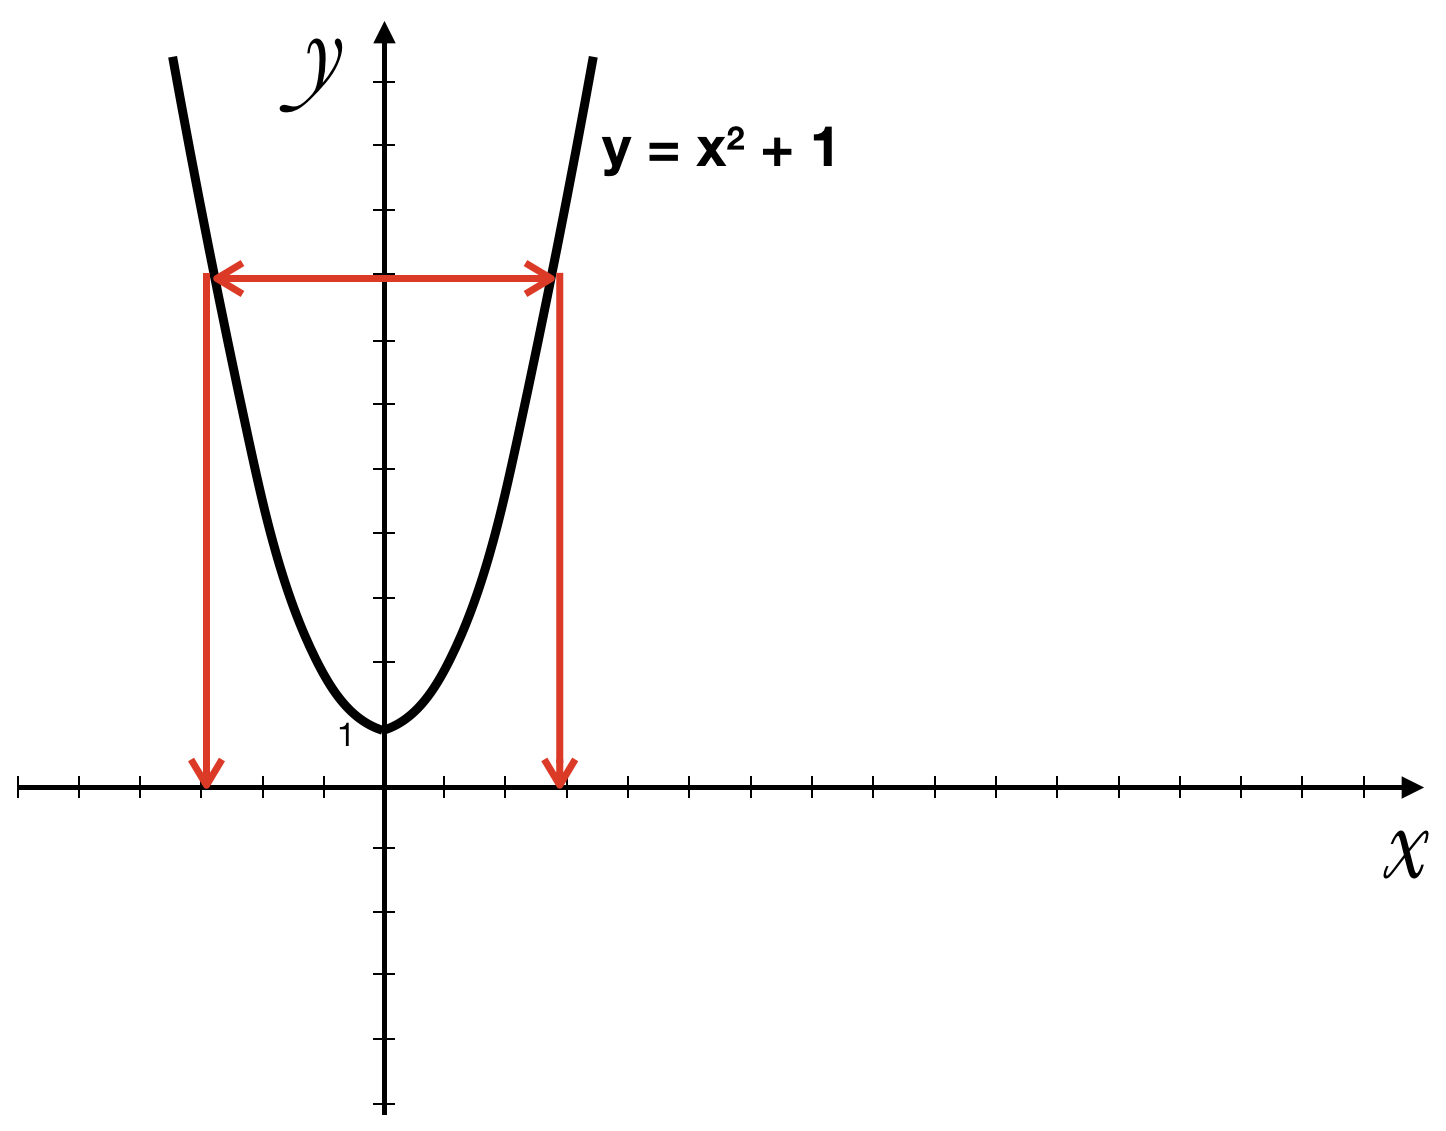
\includegraphics[width=0.7\textwidth]{img/funz_14a.png} \quad
  
%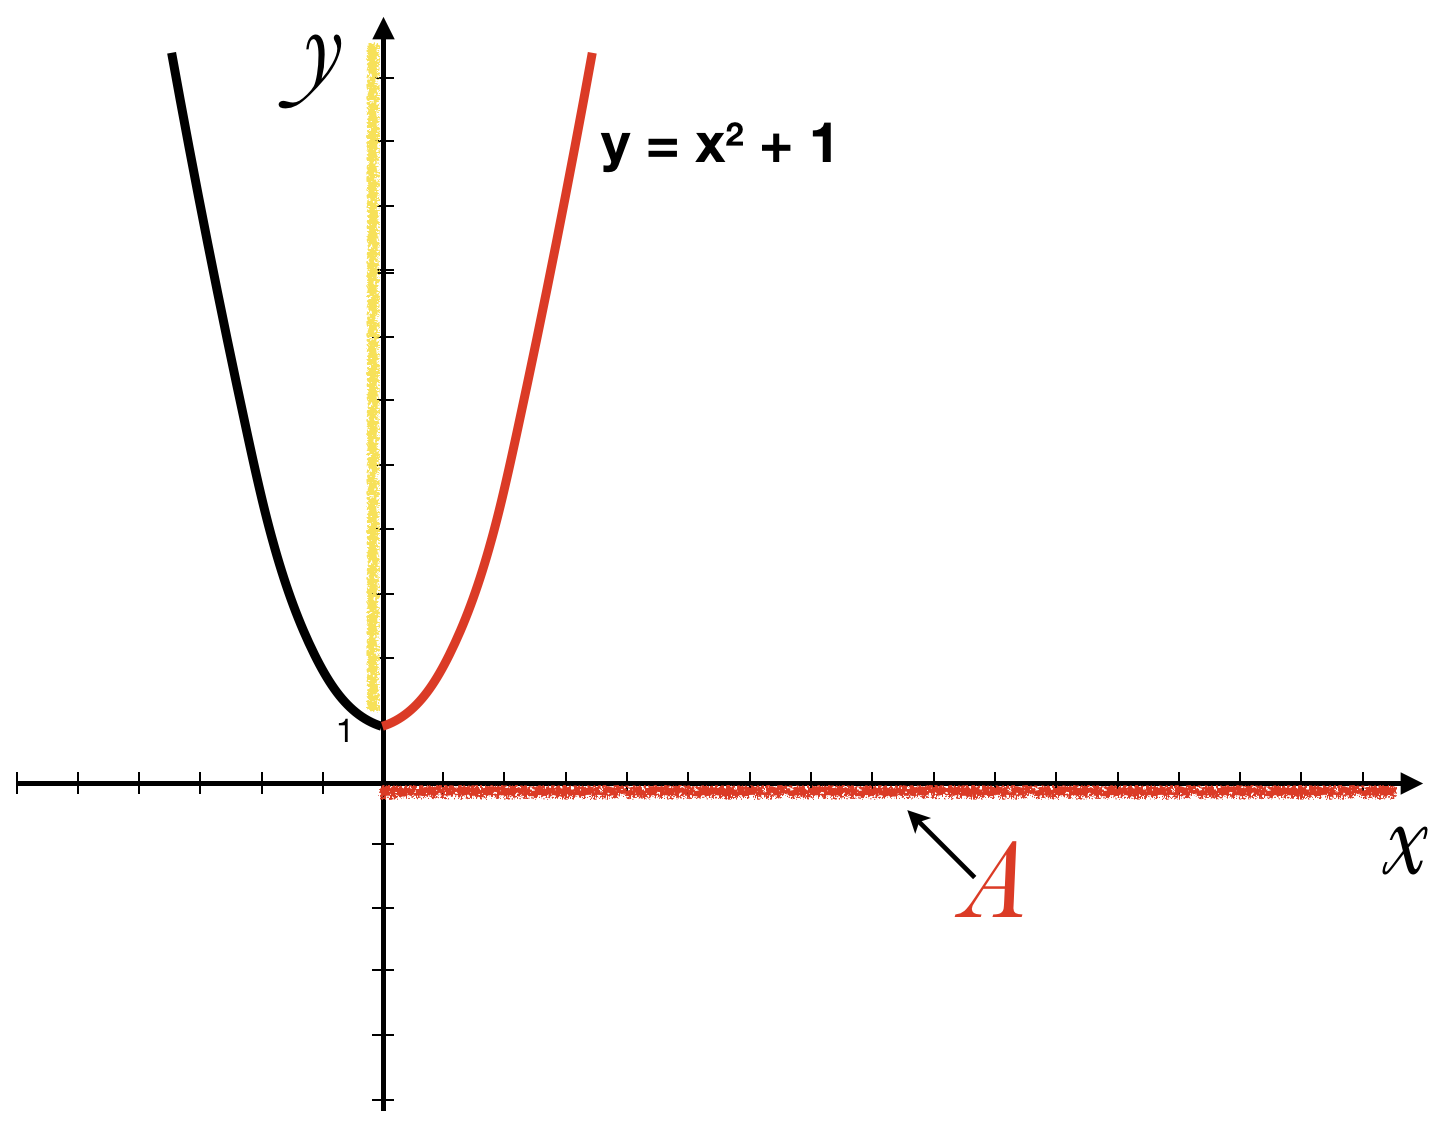
\includegraphics[width=0.7\textwidth]{img/funz_14b.png} %\quad
  
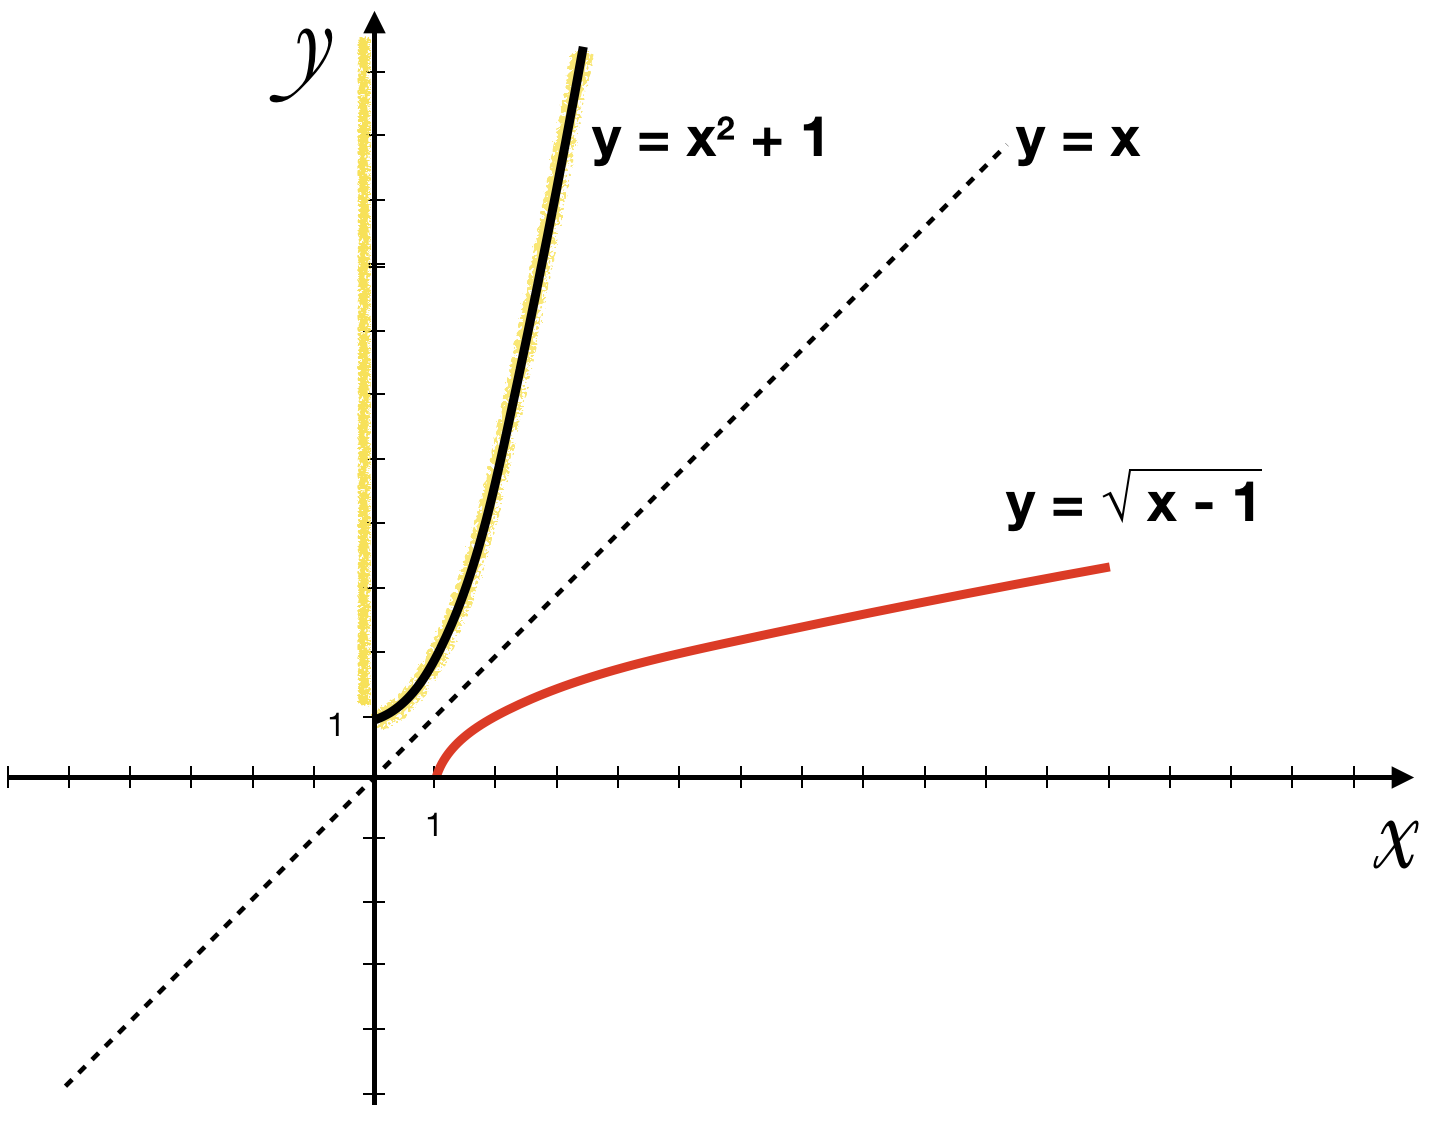
\includegraphics[width=0.45\textwidth]{img/funz_14c.png} 
  %\caption{}
  %\label{fig:funz_14abc}
  \end{figure}
\end{itemize}
\end{esempio}

Come visto negli esempi precedenti, il grafico della funzione $f^{-1}$, 
inversa della funzione $f$, è il simmetrico di $f$ rispetto alla bisettrice 
del primo e terzo quadrante.\\

Anche se sappiamo che l'inversa di una certa funzione deve essere simmetrica 
rispetto ad essa, trovare l'inversa di una determinata funzione e in 
particolar modo la sua forma analitica può non essere immediato. Forniamo 
quindi una procedura.\\

%\begin{procedura}
\textbf{Procedura 1.1} Determinare l'inversa di una funzione data:% 
\textcolor{blue}{[vedi la procedura a pag 100 vol3]}
\begin{enumerate}
  \item Si verifica che $f(x)$ è invertibile;
  \item Si esplicita la $f$ rispetto a $x$;
  \item Nella forma appena trovata si sostituisce $x$ con $y$ e $y$ con 
$x$.
\end{enumerate}
%end{procedura}
  
\begin{esempio}
Invertiamo la funzione: $f(x)=y=\sqrt[3]{x}-1$
\begin{enumerate}
  \item La funzione è invertibile perché è strettamente crescente in 
tutto il dominio $\mathbb{R}$.
  \item Esplicitiamo la funzione rispetto a $x$:\\
   $y=\sqrt[3]{x}-1\rightarrow y+1=\sqrt[3]{x}\rightarrow(y+1)^3=x$
  \item Infine otteniamo: $f^{-1}(x)=y=(x+1)^3$
\end{enumerate}
\end{esempio}

\begin{esempio}
Invertiamo la funzione: $f(x)=y=e^{x+1}-1$
\begin{enumerate}
  \item La funzione è invertibile perché è strettamente crescente in 
$\mathbb{R}$.
  \item Esplicitiamo la funzione rispetto a $x$:\\
   $y=e^{x+1}-1\rightarrow y+1=e^{x+1}\rightarrow 
\ln(x+1)=\ln(e^{x+1})\rightarrow \ln(y+1)-1=x$.\item Infine otteniamo: 
$f^{-1}(x)=y=\ln(x+1)-1$.
\end{enumerate}
\end{esempio}

Studiate le funzioni inverse discutiamo ora un'operazione tra funzioni che ci 
consentirà di creare funzioni complesse a partire da funzioni semplici: 
questa operazione si chiama \textsc{composizione di funzioni} e il suo 
risultato sarà una nuova funzione detta composta.\\

%
\begin{definizione} 
Date le funzioni $f : A\to B$ e $g : B\to C$ si dice funzione composta 
$f\circ g$ la funzione:   $(g\circ f)(x)=g(f(x))$ che associa ad ogni 
elemento di $A$ un elemento di $C$ in modo che
  \begin{itemize}
  \item all'elemento $x\in A$ corrisponde mediante $f$, 
l'elemento $f(x)\in B$
  \item all'elemento $f(x)\in B$ corrisponde, mediante $g$, 
l'elemento $g(f(x))\in C$
  \end{itemize}
affinché sia possibile calcolare $g(f(x))$, $f(x)$ deve appartenere al 
dominio di $g$. Il dominio di $g\circ f$ è costituito da tutti gli elementi 
del dominio di $f$ tali che $f(x)$ appartiene al dominio di $g$.
\end{definizione}

\begin{figure}[htpb!]
  \centering
  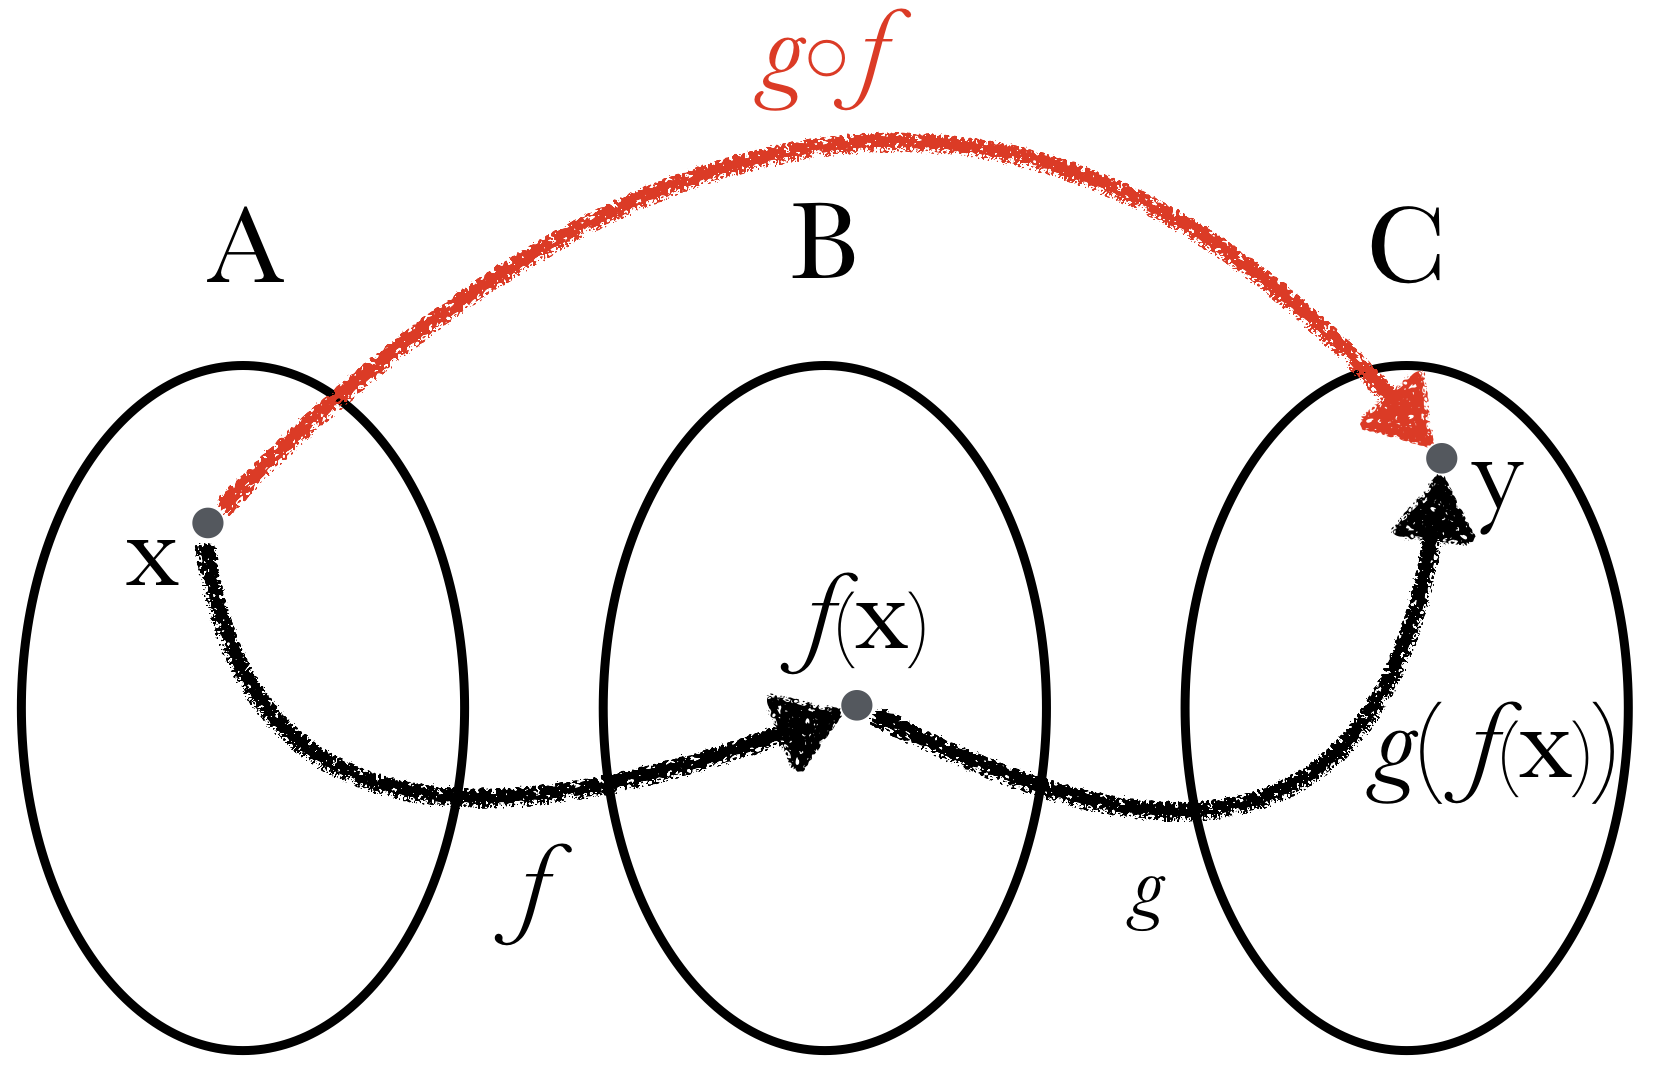
\includegraphics[width=0.55\textwidth]{img/funz_15.png} 
  %\caption{}
  %\label{fig:funz_14abc}
\end{figure}
%

La simbologia $g\circ f$ si legge <<$g$ composto $f$>> o <<$g$ dopo $f$>>; 
$g(f(x))$ si legge <<$g$ di $f$ di $x$>>.\\
 
Per quanto riguarda le proprietà di questa operazione tra funzioni notiamo 
che la composizione è associativa: $(f\circ g)\circ h=f\circ (g\circ h)$, ma 
in generale non commutativa $g\circ f\neq f\circ g.$ \\

\begin{esempio} 
Date le due funzioni $f(x)=\sqrt{x}$ e $g(x)= x+5$, determiniamo le funzioni 
composte $g\circ f$ e $f\circ g$.
Abbiamo $g\circ f=g(f(x))=g(\sqrt{x})=\sqrt{x}+5$ e il dominio  della 
funzione ottenuta è $x\geq0$. Otteniamo l'altra composta con un procedimento 
analogo $f\circ g=f(g(x))=f(x+5)=\sqrt{x+5}$ e il suo dominio è $x\geq5$. La 
diversità delle due funzioni ottenute ci conferma la non commutatività 
dell'operazione di composizione.\\
\end{esempio}

\textbf{Posso comporre una funzione con la sua inversa?}\\
Sia $f$ una funzione invertibile di dominio $D$ e immagine $I$, con $f^{-1} $ 
la sua inversa.
Consideriamo la composta $f^{-1}\circ f$, cioè $f^{-1}$ dopo $f$: $x$ va in 
$f(x)$ che a sua volta va in $x$, $f^{-1}(f(x))=x$, $\forall x\in D$ 
$f^{-1}\circ f$ è la funzione identità in $D$, analogamente anche 
$f(f^{-1}(x))=x$, $f\circ f^{-1}$ è l'identità in $I$. Ricordiamo che la 
funzione identità è una particolare funzione che associa ad ogni $x$ la $x$ 
stessa, cioè associa ad ogni elemento del dominio, lo stesso elemento nel 
codominio.\\

\begin{definizione}
Due funzioni $f$ e $g$ si dicono uguali se hanno lo stesso dominio $D$ e 
risulta $$f(x)=g(x)$$ $\forall x\in D$.\\
\end{definizione}
 
\begin{esempio}
Vediamo un esempio di funzioni uguali e non uguali. Le due funzioni
$$f(x)=\frac{\sqrt{x}}{\sqrt{x^2+4}}$$ e $$g(x)=\sqrt{\frac{x}{x^2+4}}$$
sono uguali perchè hanno lo stesso dominio ($x\geq0$) e risulta:
$$\frac{\sqrt{x}}{\sqrt{x^2+4}}=\sqrt{\frac{x}{x^2+4}}$$ per ogni $x\geq0$.
Vediamo un contoesempio di funzioni uguali. Le due funzioni
$$f(x)=\frac{\sqrt{x}}{\sqrt{x+4}}$$ e $$g(x)=\sqrt{\frac{x}{x+4}}$$
non sono uguali perché hanno dominio diverso: la funzione $f$ è definita per 
$x\geq0$, mentre la funzione $g$ è definita per $x<-4\lor x\geq 0$.
$$\frac{\sqrt{x}}{\sqrt{x^2+4}}=\sqrt{\frac{x}{x^2+4}}$$ per ogni $x\geq0$.
\end{esempio}


\end{comment}








